\documentclass[compress]{beamer}
\usepackage{ifthen,verbatim}

\newcommand{\isnote}{}
\xdefinecolor{lightyellow}{rgb}{1.,1.,0.25}
\xdefinecolor{darkblue}{rgb}{0.1,0.1,0.7}

%% Uncomment this to get annotations
%% \def\notes{\addtocounter{page}{-1}
%%            \renewcommand{\isnote}{*}
%% 	   \beamertemplateshadingbackground{lightyellow}{white}
%%            \begin{frame}
%%            \frametitle{Notes for the previous page (page \insertpagenumber)}
%%            \itemize}
%% \def\endnotes{\enditemize
%% 	      \end{frame}
%%               \beamertemplateshadingbackground{white}{white}
%%               \renewcommand{\isnote}{}}

%% Uncomment this to not get annotations
\def\notes{\comment}
\def\endnotes{\endcomment}

\setbeamertemplate{navigation symbols}{}
\setbeamertemplate{headline}{\mbox{ } \hfill
\begin{minipage}{5.5 cm}
\vspace{-0.75 cm} \small
\end{minipage} \hfill
\begin{minipage}{4.5 cm}
\vspace{-0.75 cm} \small
\begin{flushright}
\ifthenelse{\equal{\insertpagenumber}{1}}{}{Jim Pivarski \hspace{0.2 cm} \insertpagenumber\isnote/\pageref{numpages}}
\end{flushright}
\end{minipage}\mbox{\hspace{0.2 cm}}\includegraphics[height=1 cm]{../cmslogo} \hspace{0.1 cm} \includegraphics[height=1 cm]{../tamulogo} \hspace{0.01 cm} \vspace{-1.05 cm}}

\newcommand{\s}[1]{{\mbox{\scriptsize #1}}}

\begin{document}
%% \begin{notes}
%% \item This is the annotated version of my talk.
%% \item If you want the version that I am presenting, download the one
%% labeled ``slides'' on Indico (or just ignore these yellow pages).
%% \item The annotated version is provided for extra detail and a written
%% record of comments that I intend to make orally.
%% \item Yellow notes refer to the content on the {\it previous} page.
%% \item All other slides are identical for the two versions.
%% \end{notes}

\small

%% \begin{frame}
%% \frametitle{Outline}
%% \begin{itemize}\setlength{\itemsep}{0.75 cm}
%% \item 
%% \end{itemize}
%% %% \hspace{-0.83 cm} \textcolor{darkblue}{\Large Outline2}
%% \end{frame}

\begin{frame}
\frametitle{Introduction}

A study of the low-$p_T$ dimuon spectrum (background control \\ sample).  Normalized by cross-section except prompt $J/\psi$ (factor of 2 too high, reduced by hand).

\textcolor{darkblue}{Baseline cuts:}
\begin{itemize}
\item exactly two opposite-sign muons per event; mass $<$ 5~GeV/$c^2$
\item one muon $p_T > 12$~GeV/$c$, $|\eta| < 1$ (for trigger)
\item the other $p_T > 5$~GeV/$c$, $|\eta| < 2.4$
\item dimuon $p_T < 80$~GeV/$c$ (where backgrounds $\gg$ 1~pb)
\end{itemize}

\begin{center}
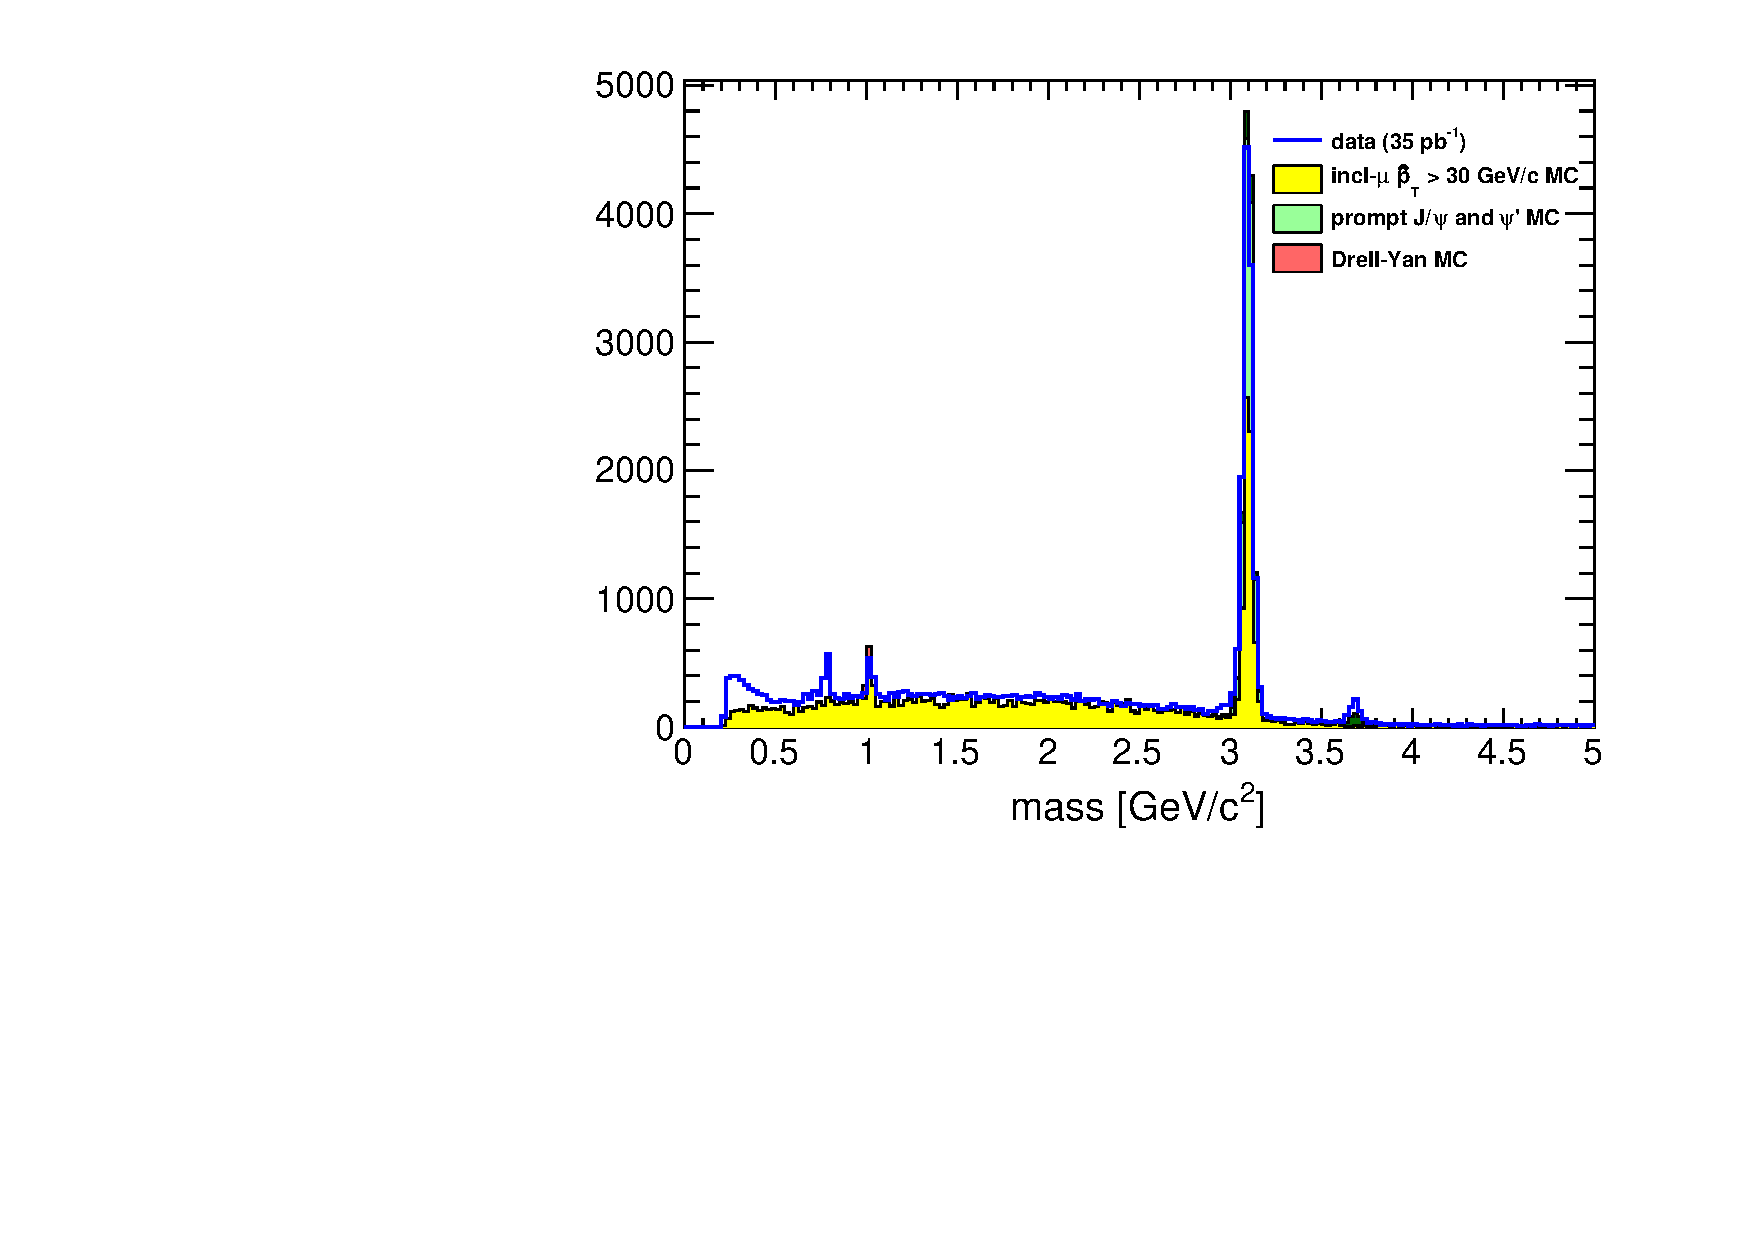
\includegraphics[width=0.6\linewidth]{lowdimuon_massdistribution.pdf}
\end{center}
\end{frame}

\begin{frame}
\frametitle{Isolation as a tool}

\[ Iso = \sum_\s{non-$\mu$ tracks} \left\{ \begin{array}{c l} p_T &
  \mbox{ if $\Delta R < 0.5$ and $p_T > 1.5$ GeV/$c$} \\ 0 &
  \mbox{ otherwise} \end{array} \right. \]

\begin{itemize}
\item ``isolated:'' $Iso < 4.5$~GeV/$c$ (first three bins)
\item ``iso-sideband:'' $4.5 < Iso < 10.5$~GeV/$c$ (next four bins)
\item ``non-isolated:'' $Iso > 10.5$~GeV/$c$ (the rest of the distribution)
\end{itemize}

\begin{center}
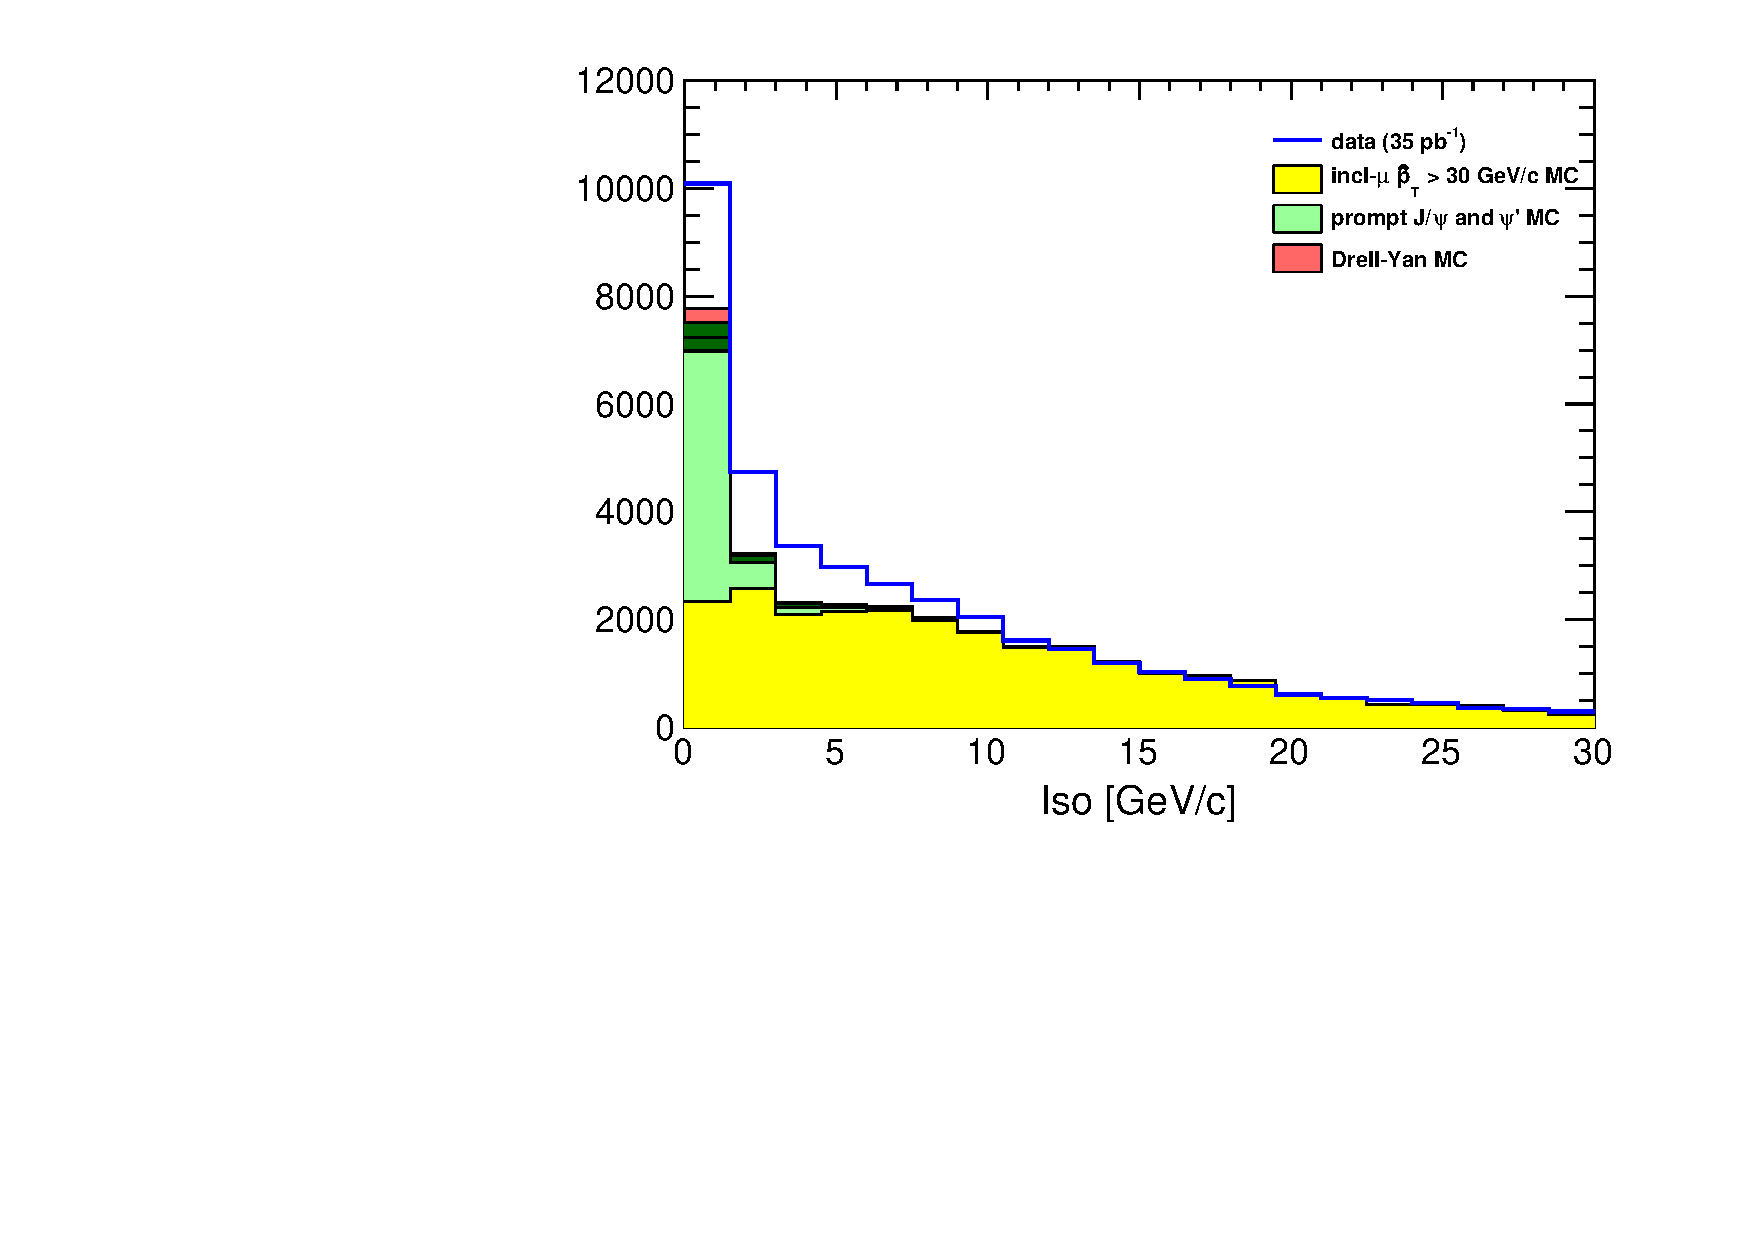
\includegraphics[width=0.6\linewidth]{lowdimuon_isodistribution.pdf}
\end{center}
\end{frame}

\begin{frame}
\frametitle{Mass in isolation bins}

\begin{columns}
\column{0.6\linewidth}
\begin{itemize}
\item Excess in isolated data across the mass spectrum (1.1 $<$ mass $<$ 2.9~GeV/$c^2$)
\item Special excess in mass $<$ 0.5~GeV/$c^2$, wider than a resonance
\end{itemize}

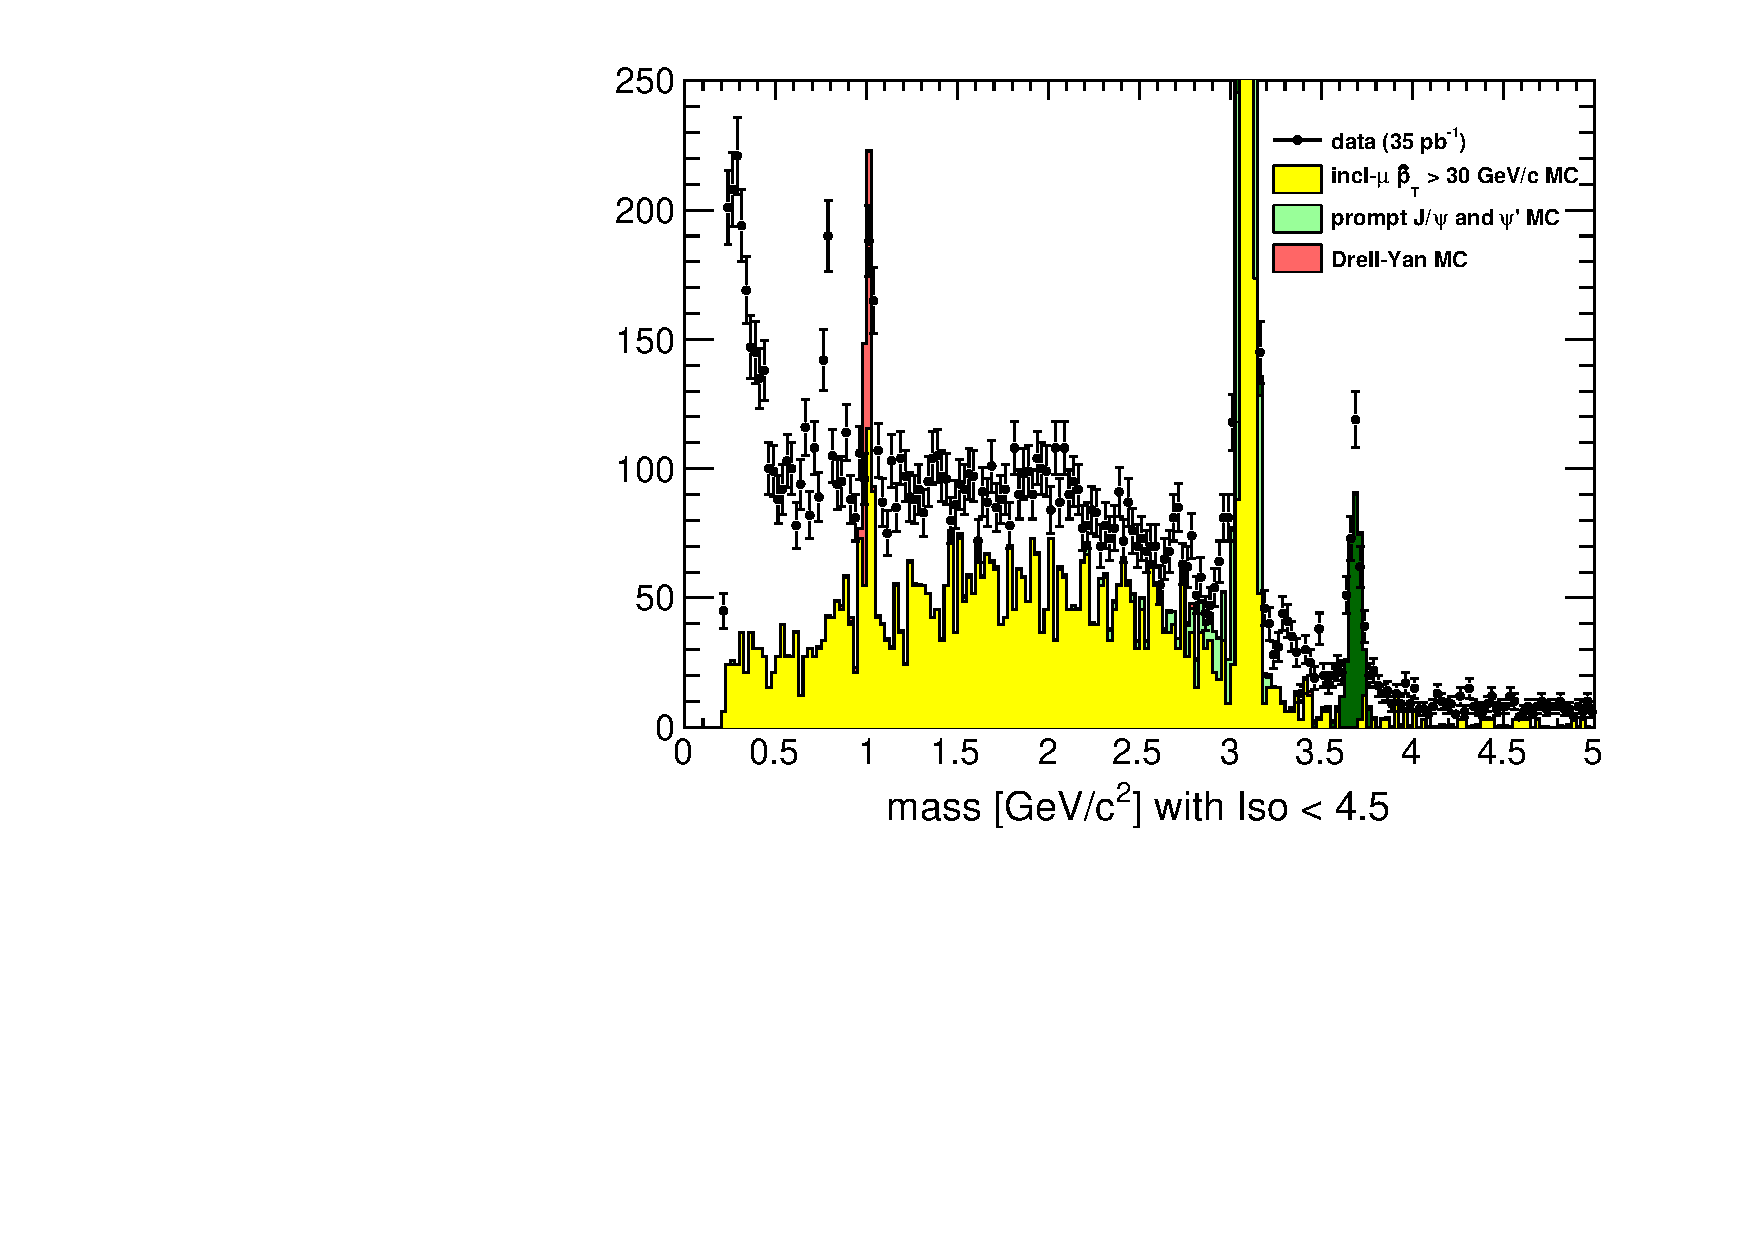
\includegraphics[width=\linewidth]{lowdimuon_mass_isolated.pdf}

\column{0.4\linewidth}
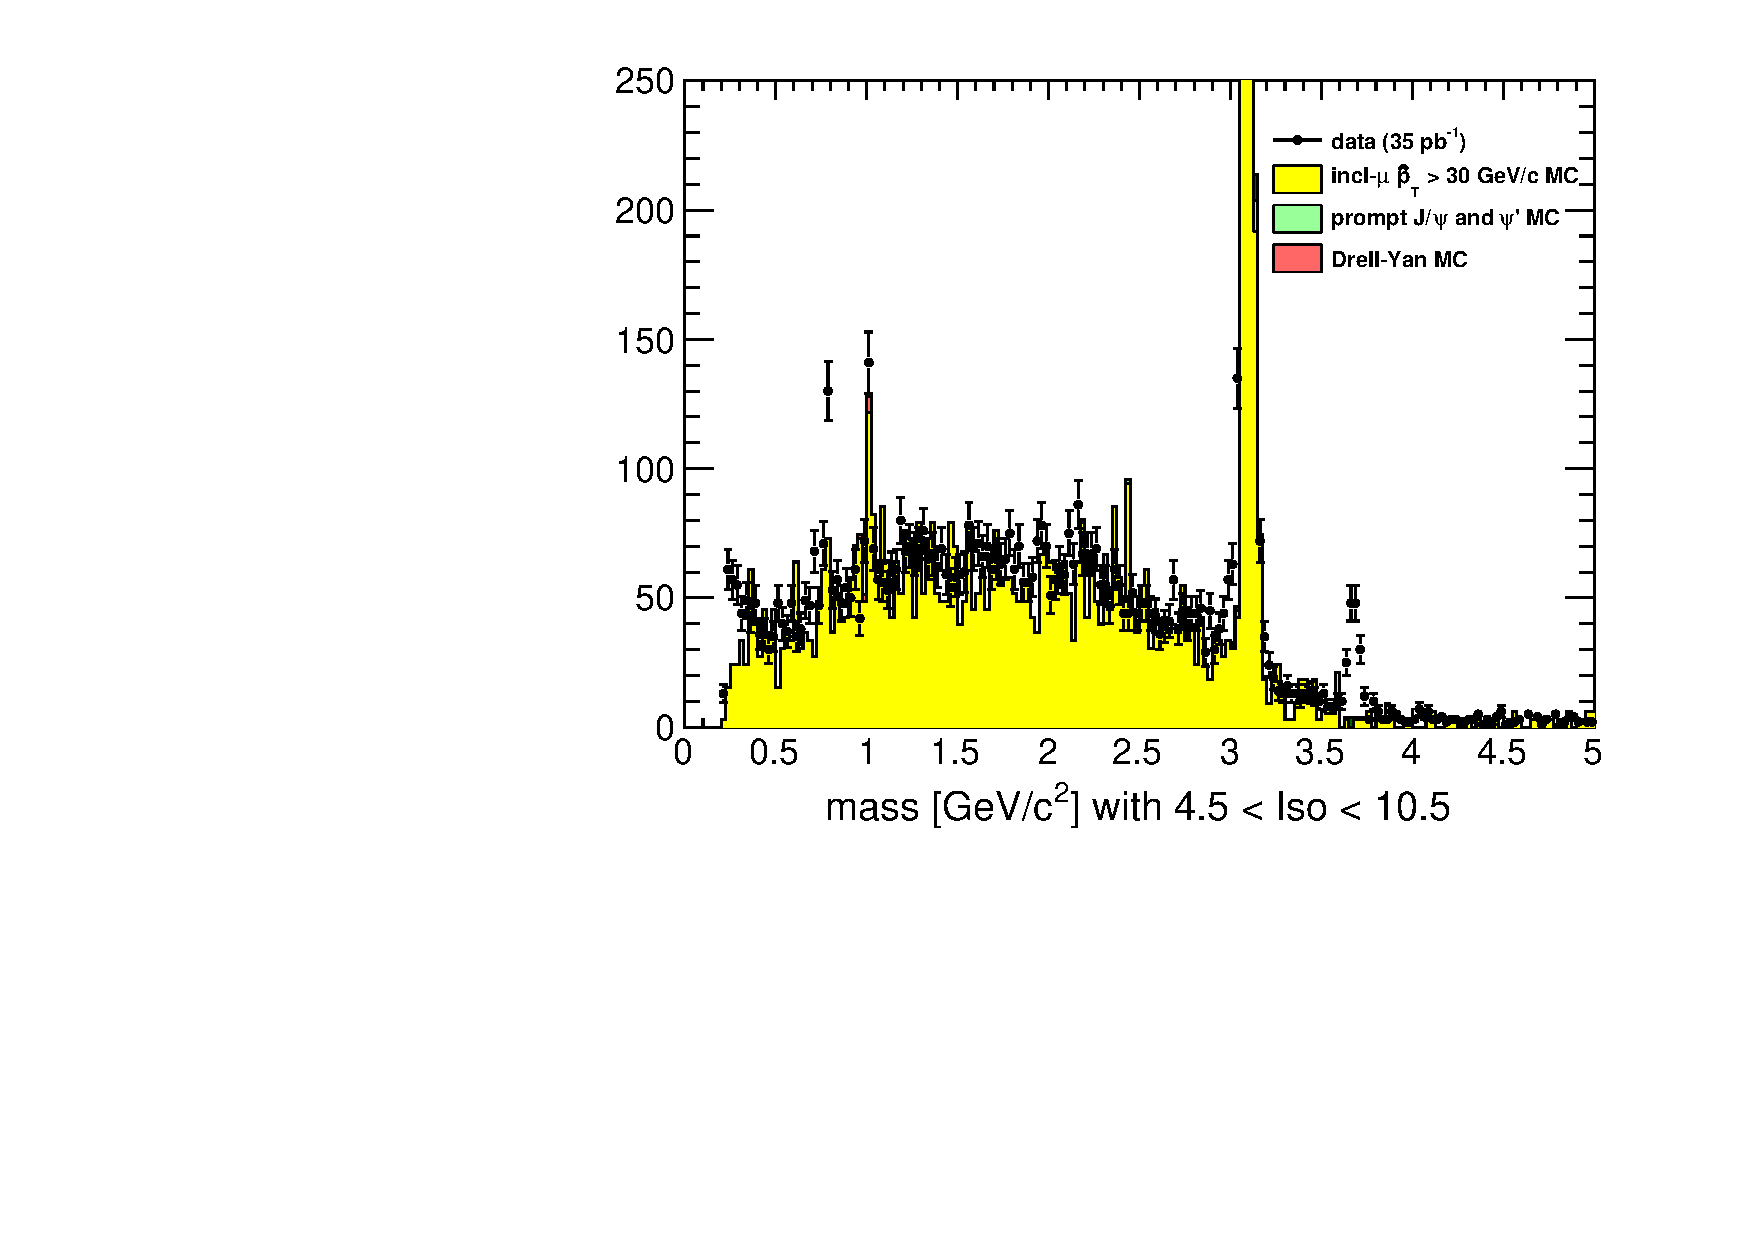
\includegraphics[width=\linewidth]{lowdimuon_mass_isosideband.pdf}

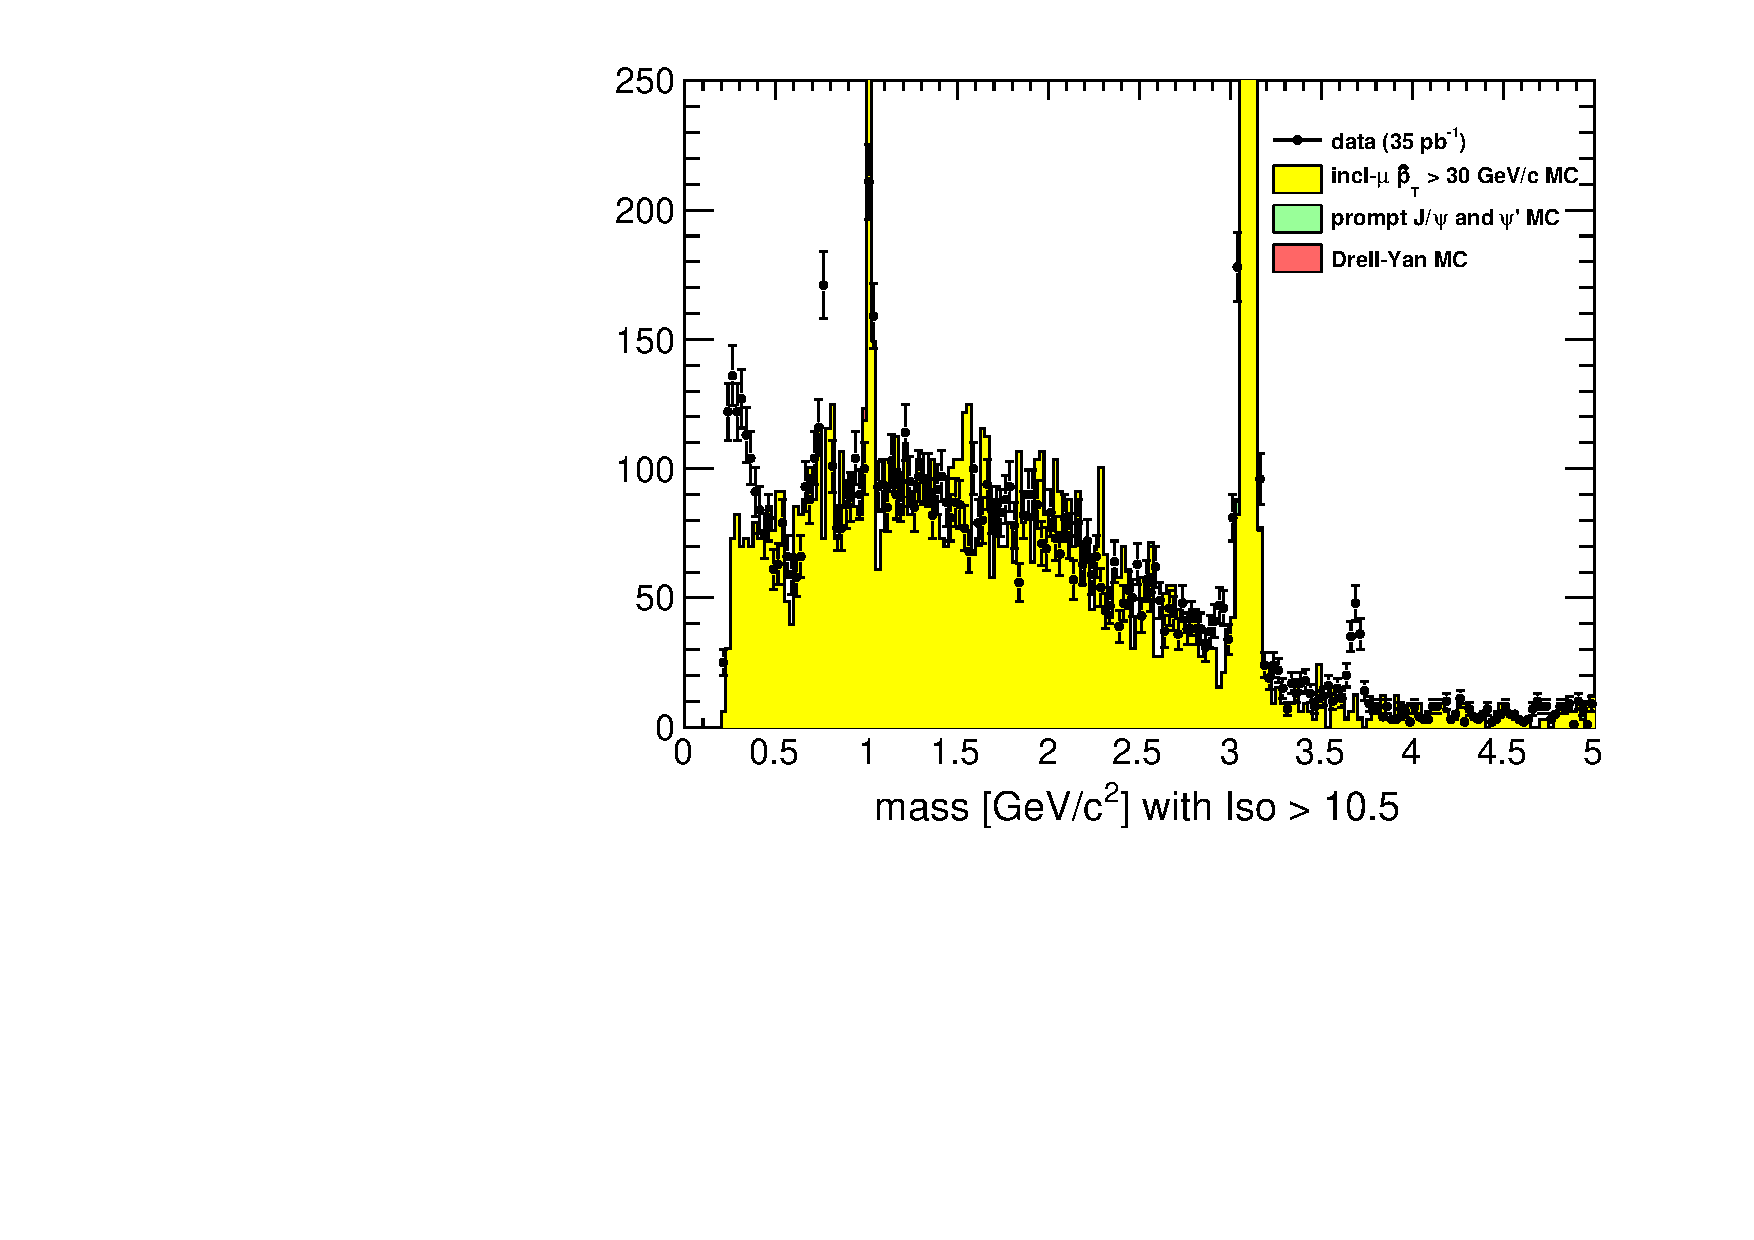
\includegraphics[width=\linewidth]{lowdimuon_mass_noniso.pdf}
\end{columns}
\end{frame}

\begin{frame}
\frametitle{It's not smearing at low mass}

\begin{itemize}
\item What if the low-mass part is due to smearing (not in the MC)?
\item Quick mass resolution plots from pair-gun
\end{itemize}

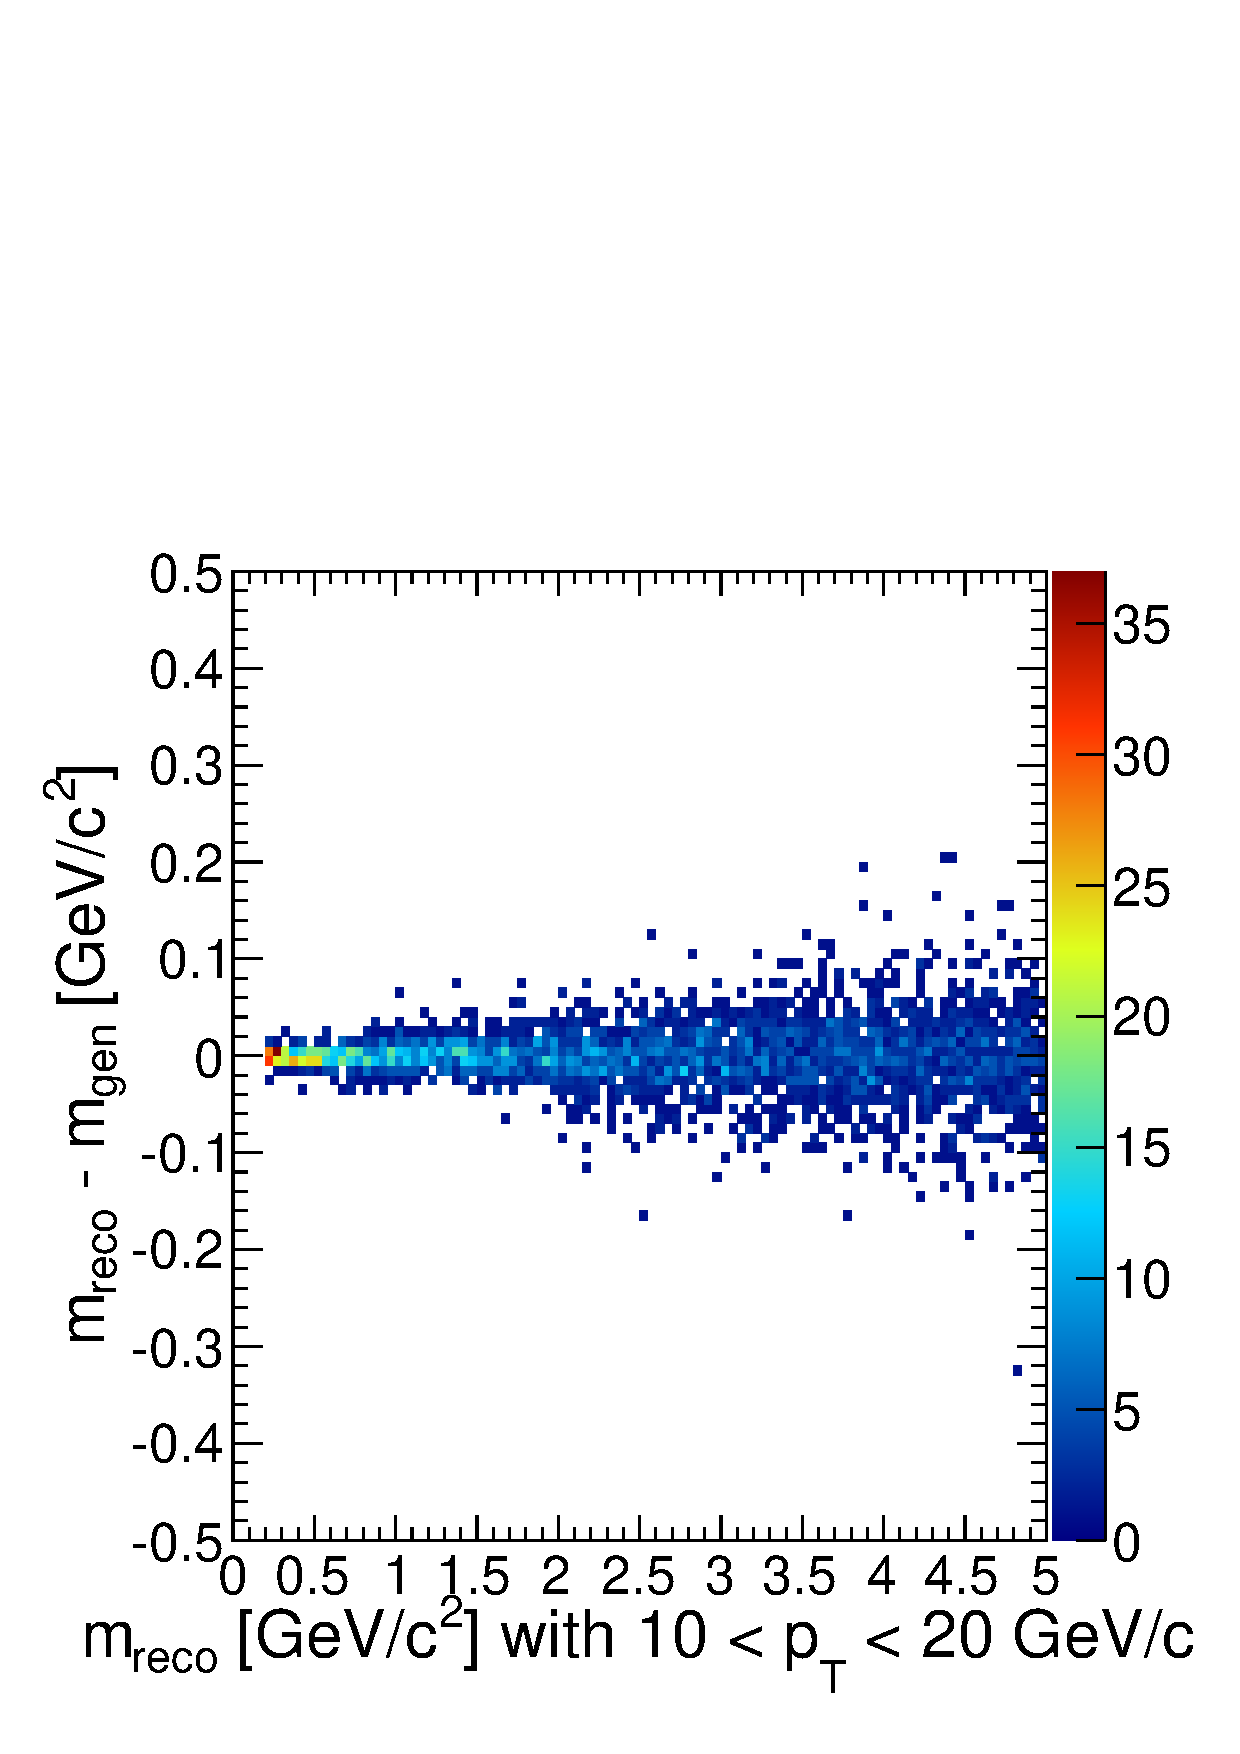
\includegraphics[width=0.32\linewidth]{massresolution_lowpt.pdf}
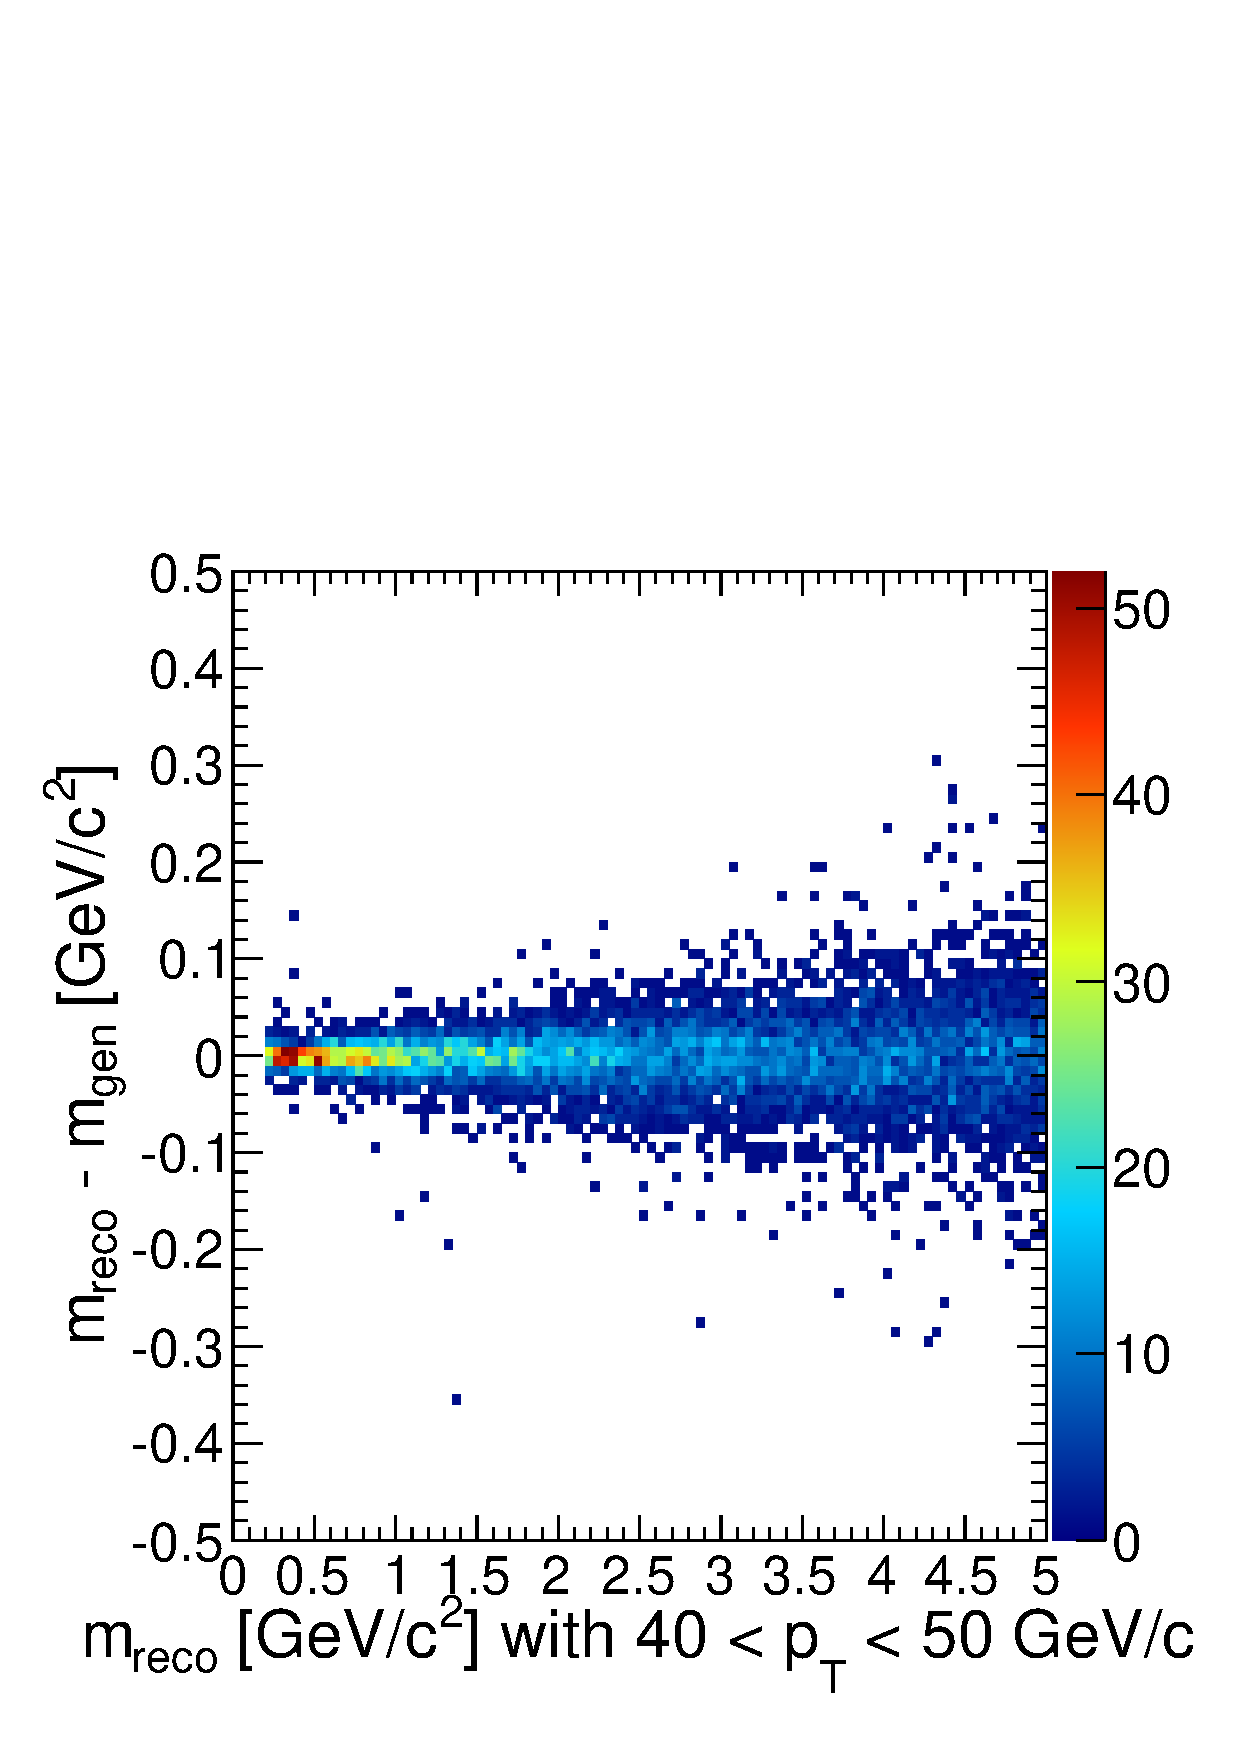
\includegraphics[width=0.32\linewidth]{massresolution_midpt.pdf}
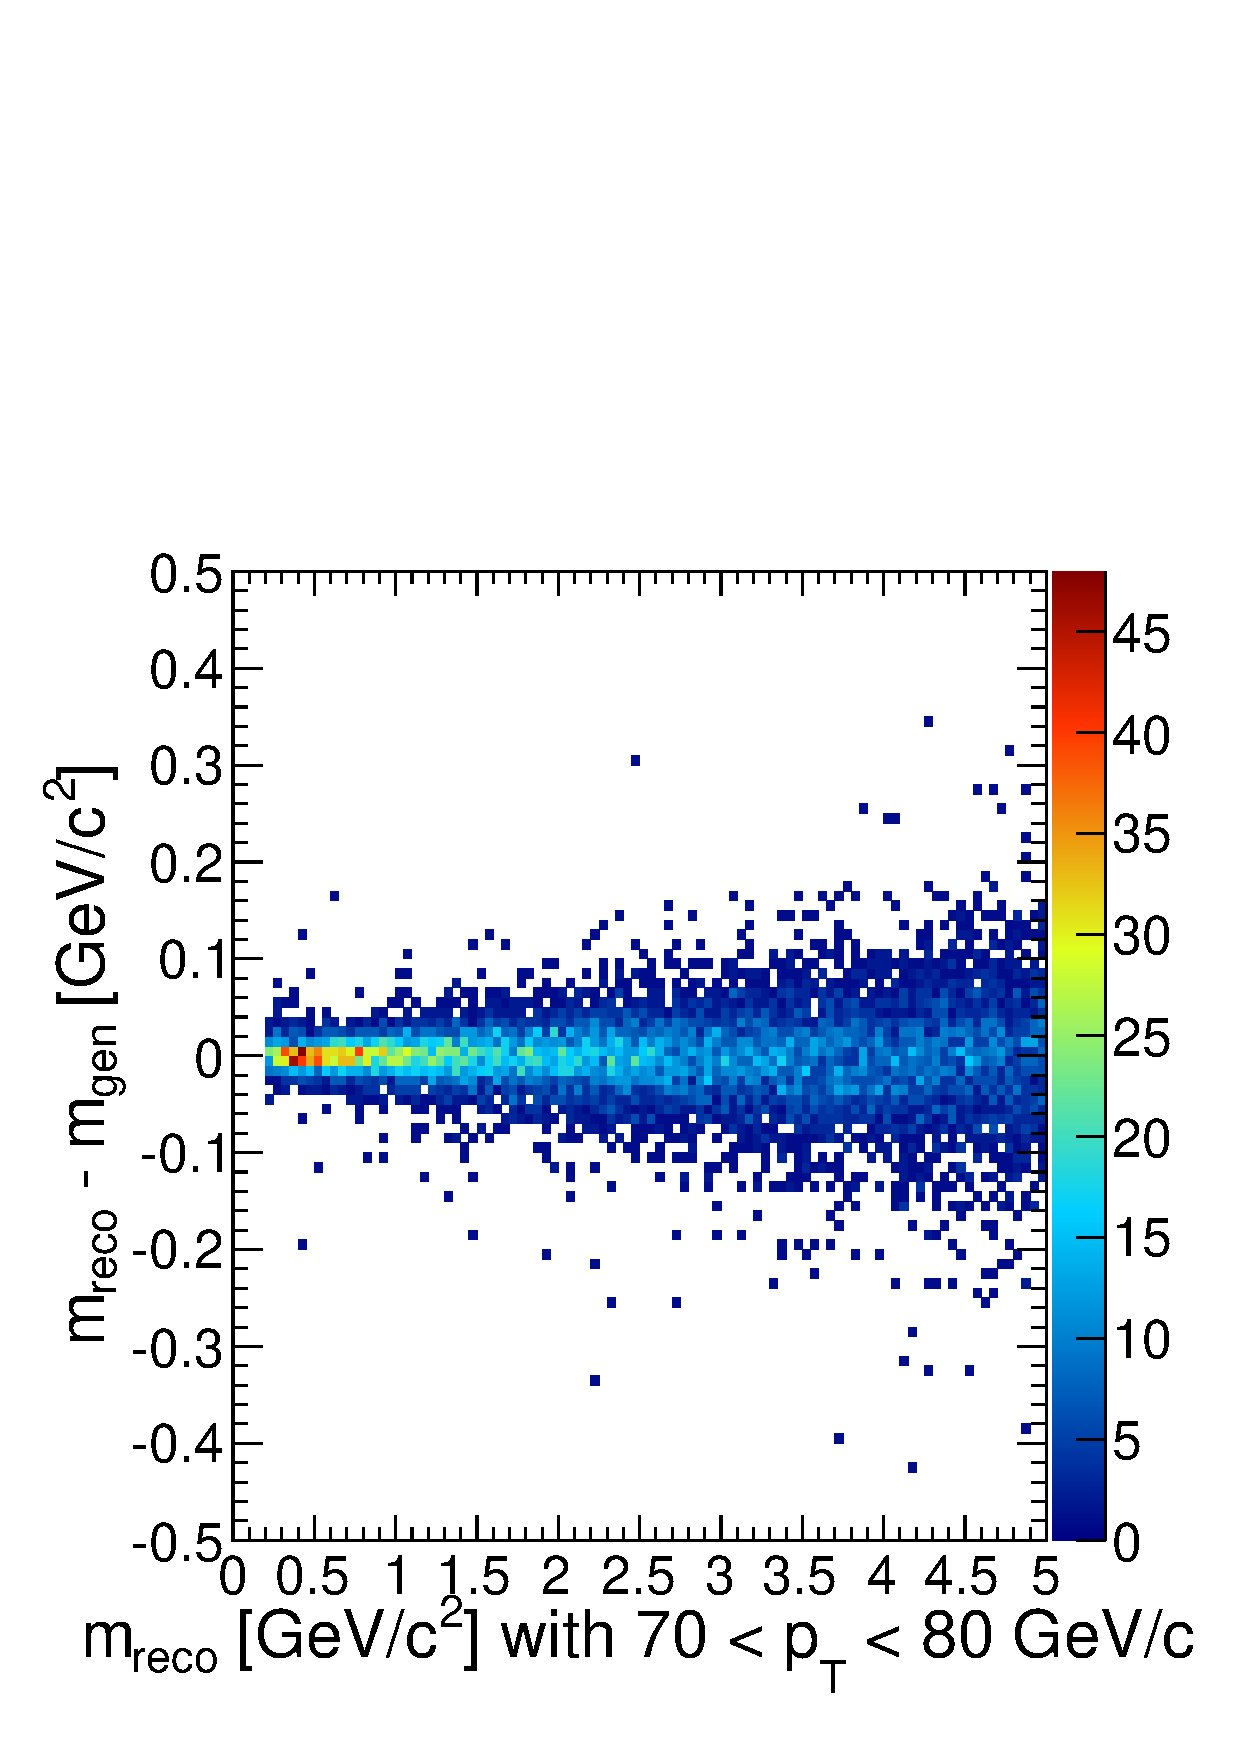
\includegraphics[width=0.32\linewidth]{massresolution_highpt.pdf}

\begin{itemize}
\item I suppose this alone doesn't prove that such a thing isn't
  happening in the real data, but we know that the $K_S$ mass peak is
  not significantly wider in data than MC
\end{itemize}
\end{frame}

\begin{frame}
\frametitle{They're not bad muons}

\begin{columns}
\column{0.6\linewidth}
\begin{itemize}
\item Compare muon quality distributions in the mass $<$ 0.5~GeV/$c^2$
  region (black) with the same distributions in the $J/\psi$ peak
  (red)
\item Normalized to equal area (all data)
\end{itemize}

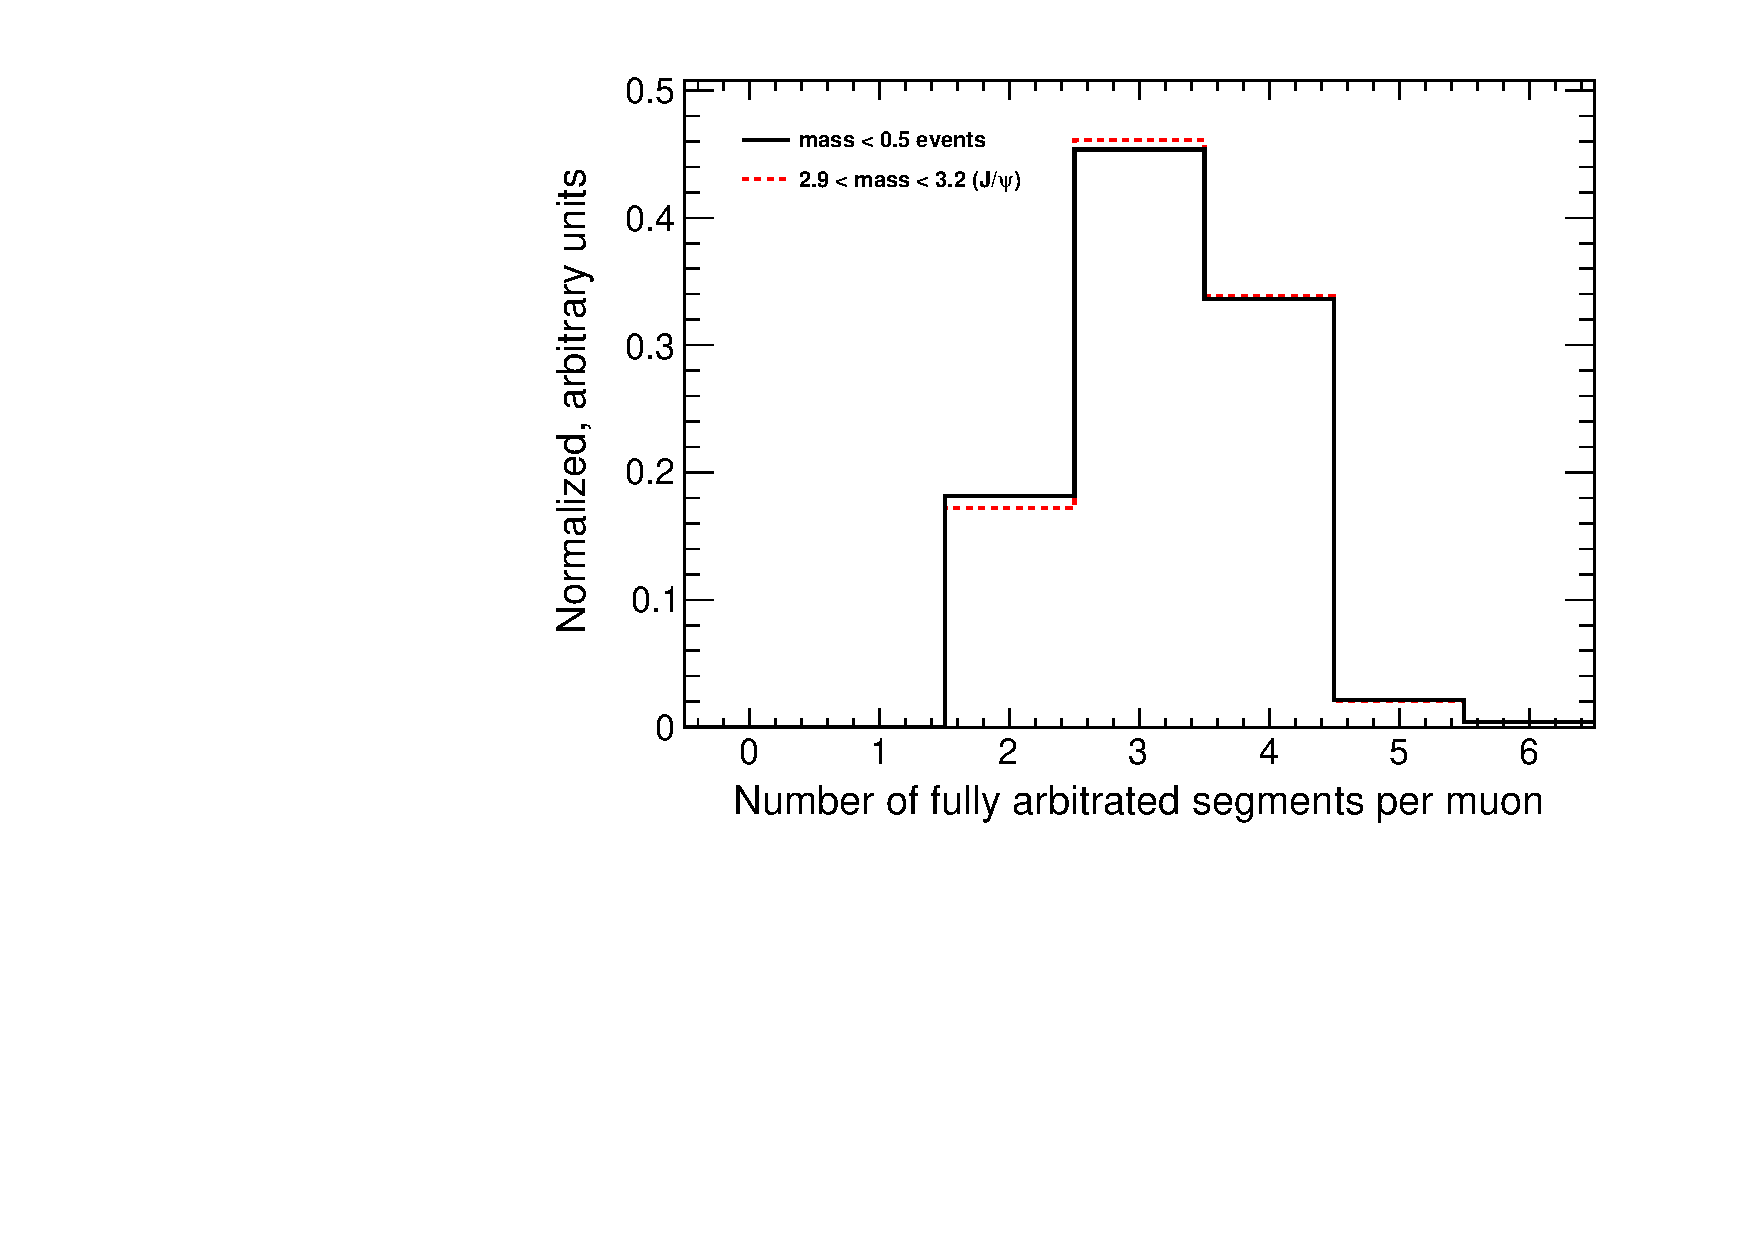
\includegraphics[width=\linewidth]{lowmassquality_matches.pdf}

\column{0.4\linewidth}
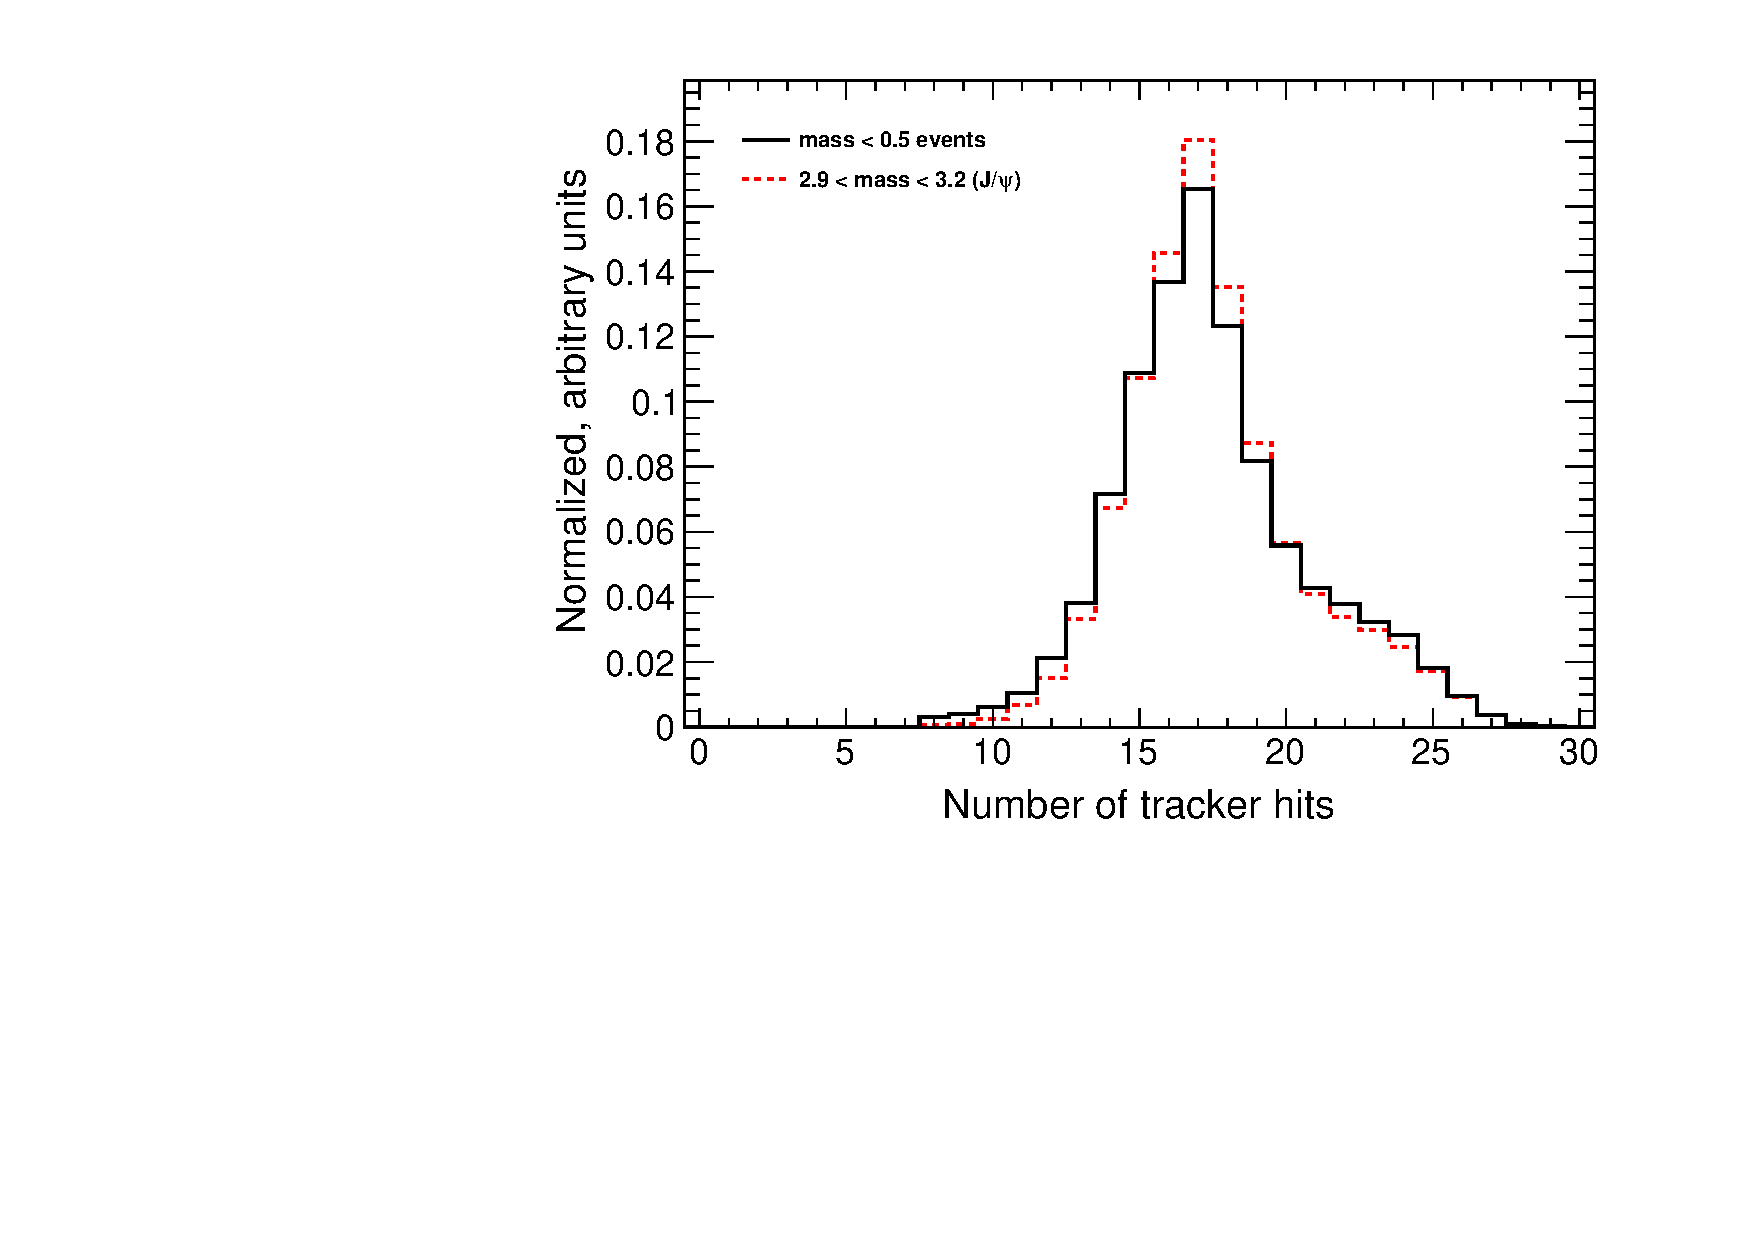
\includegraphics[width=\linewidth]{lowmassquality_hits.pdf}

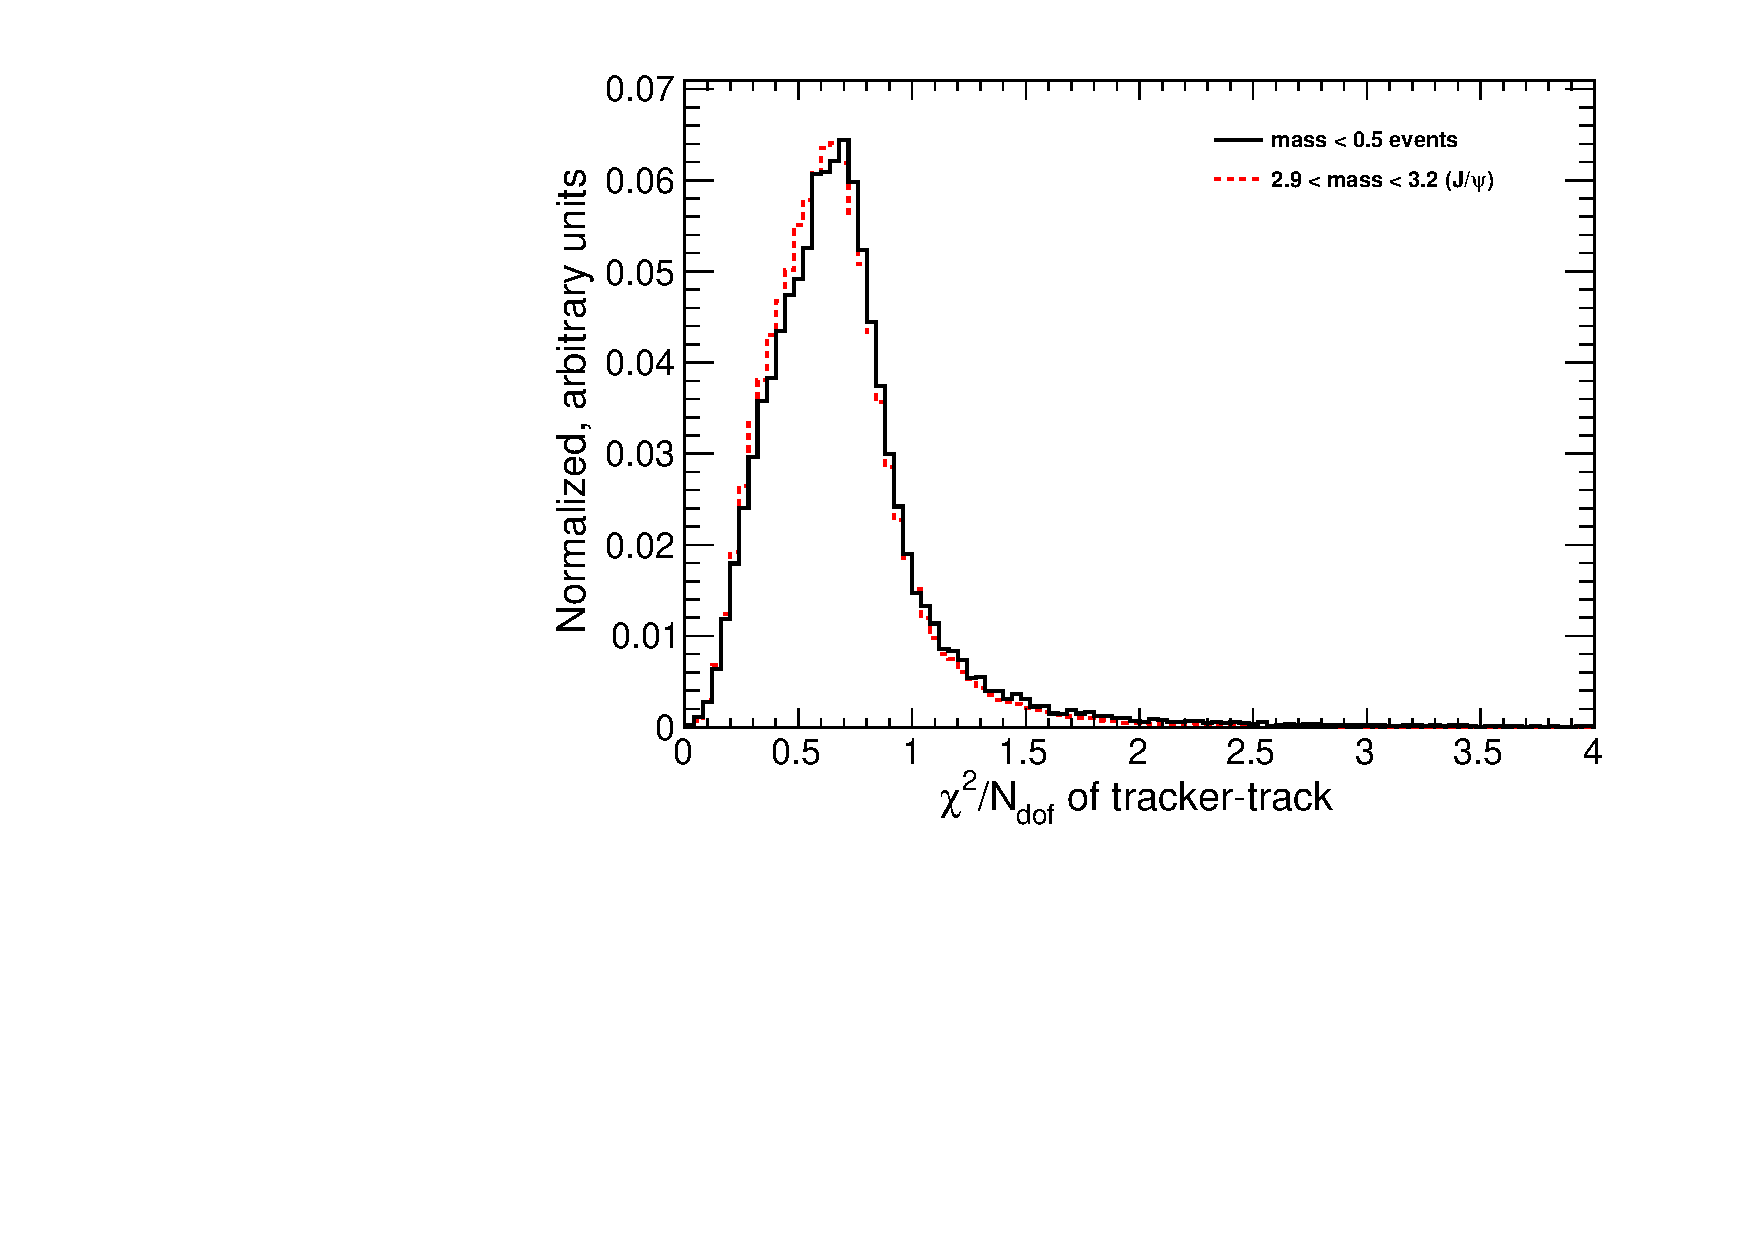
\includegraphics[width=\linewidth]{lowmassquality_normchi2.pdf}
\end{columns}
\end{frame}

\begin{frame}
\frametitle{They're not bad muons}

\begin{itemize}
\item Residuals distributions in station 1 (of both barrel and endcap)
\end{itemize}

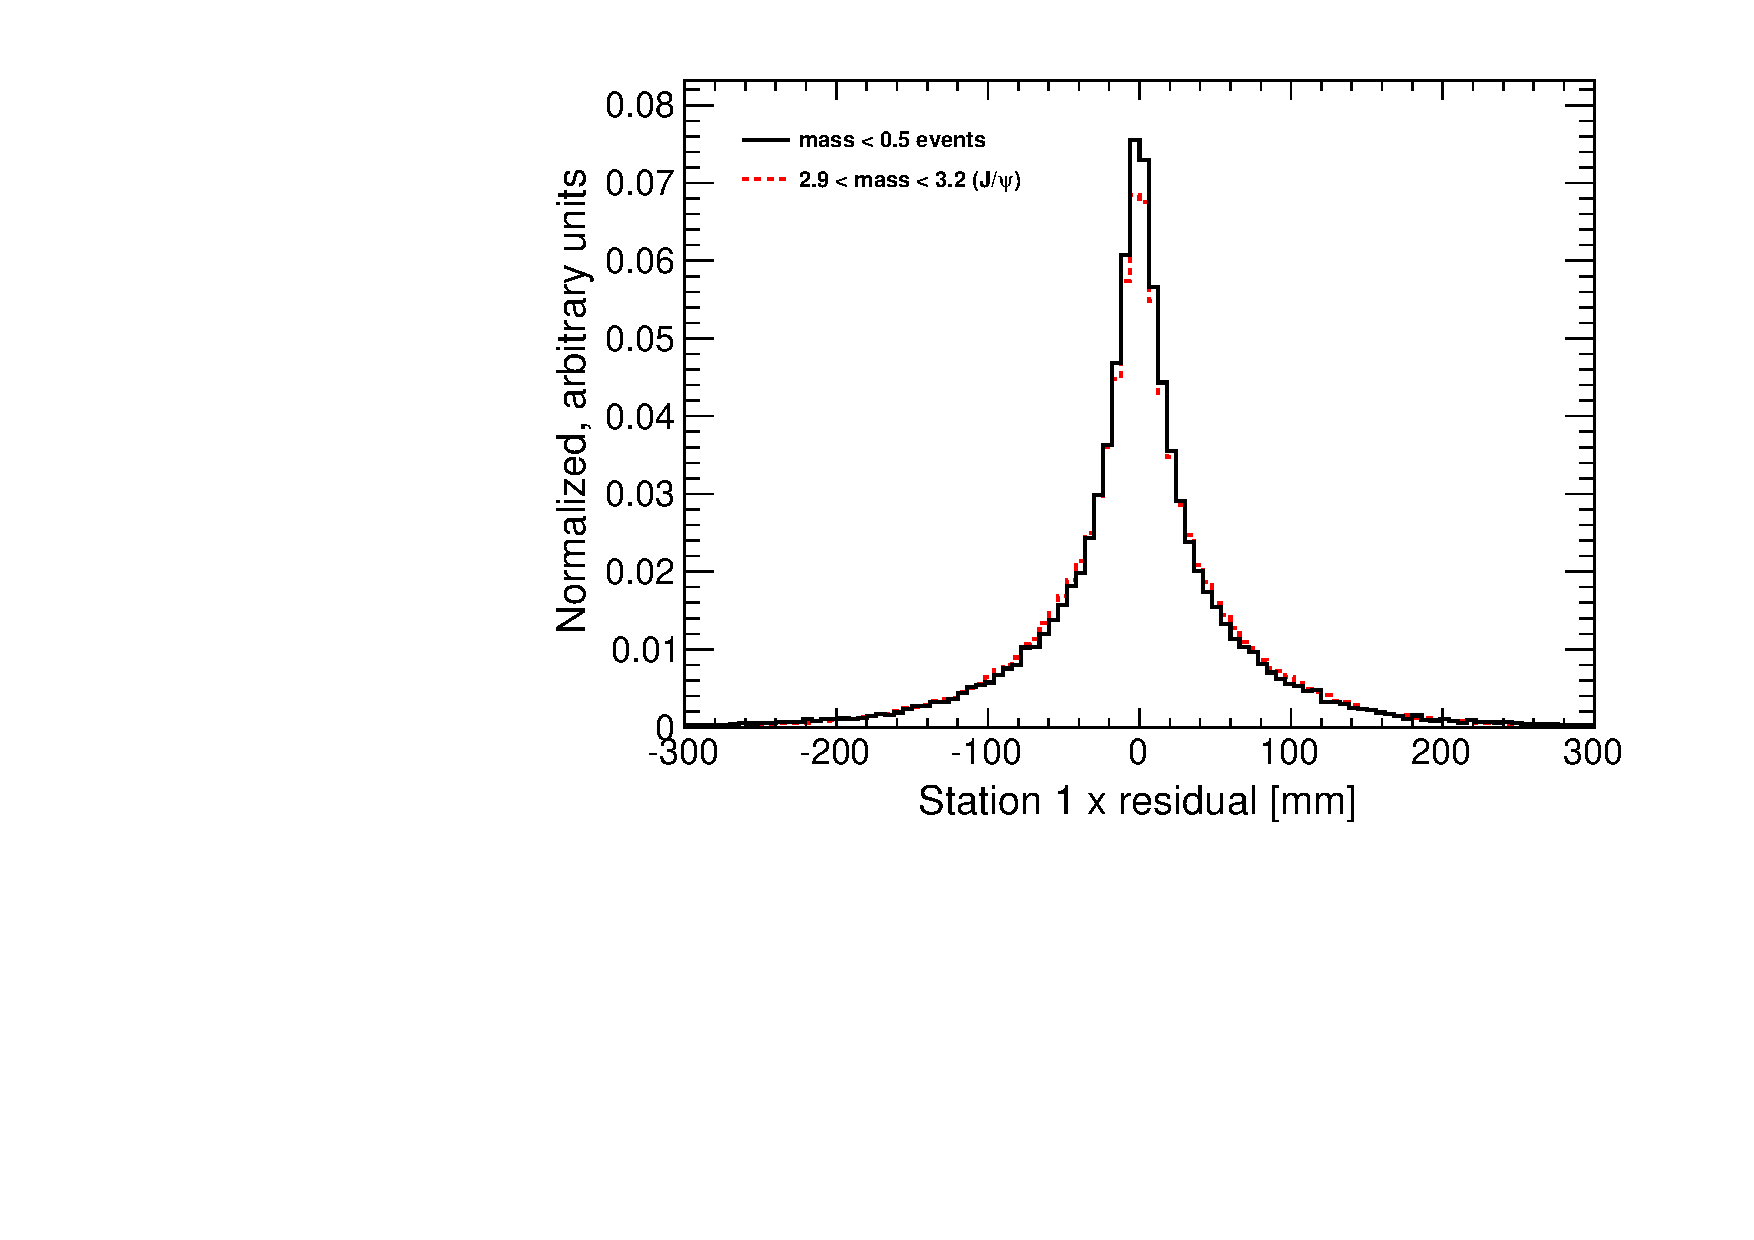
\includegraphics[width=0.45\linewidth]{lowmassquality_st1x.pdf} \hfill
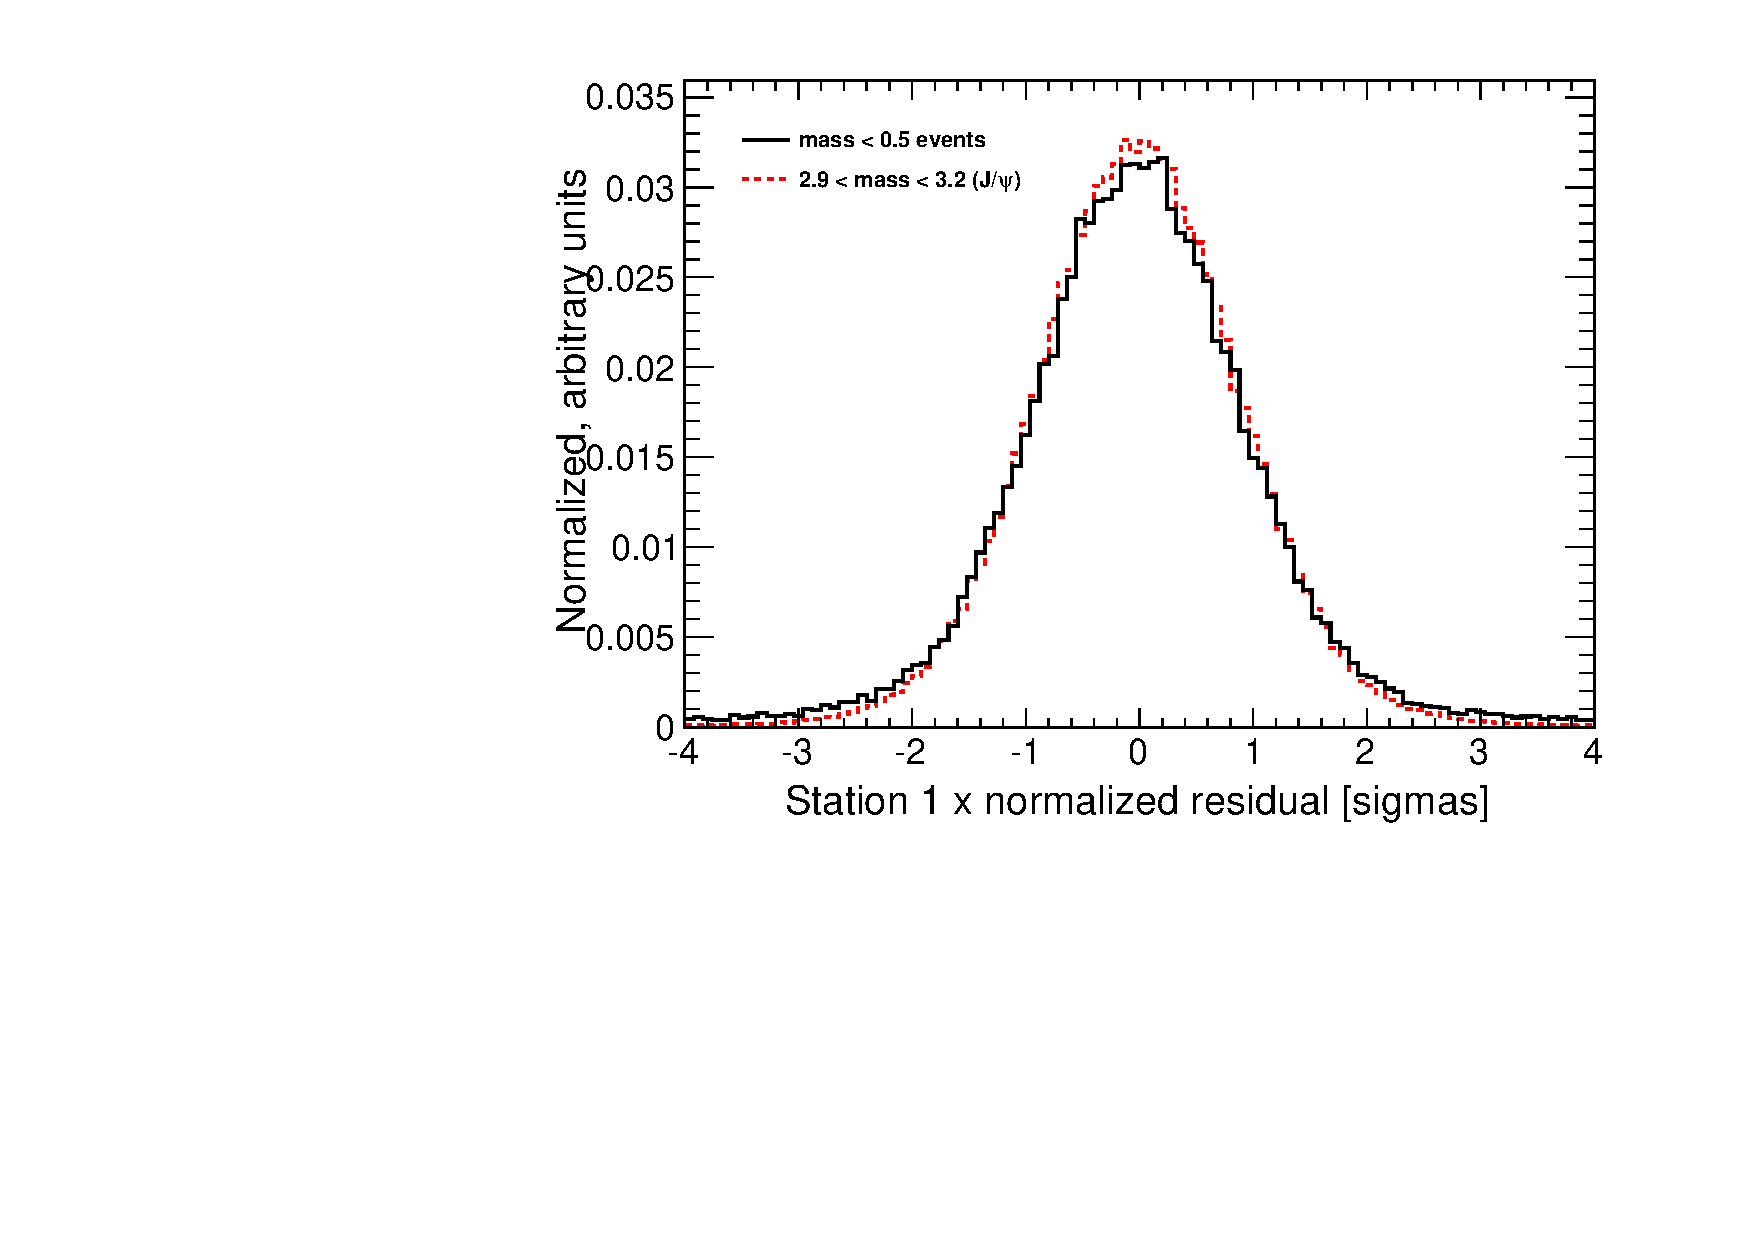
\includegraphics[width=0.45\linewidth]{lowmassquality_st1xsig.pdf}

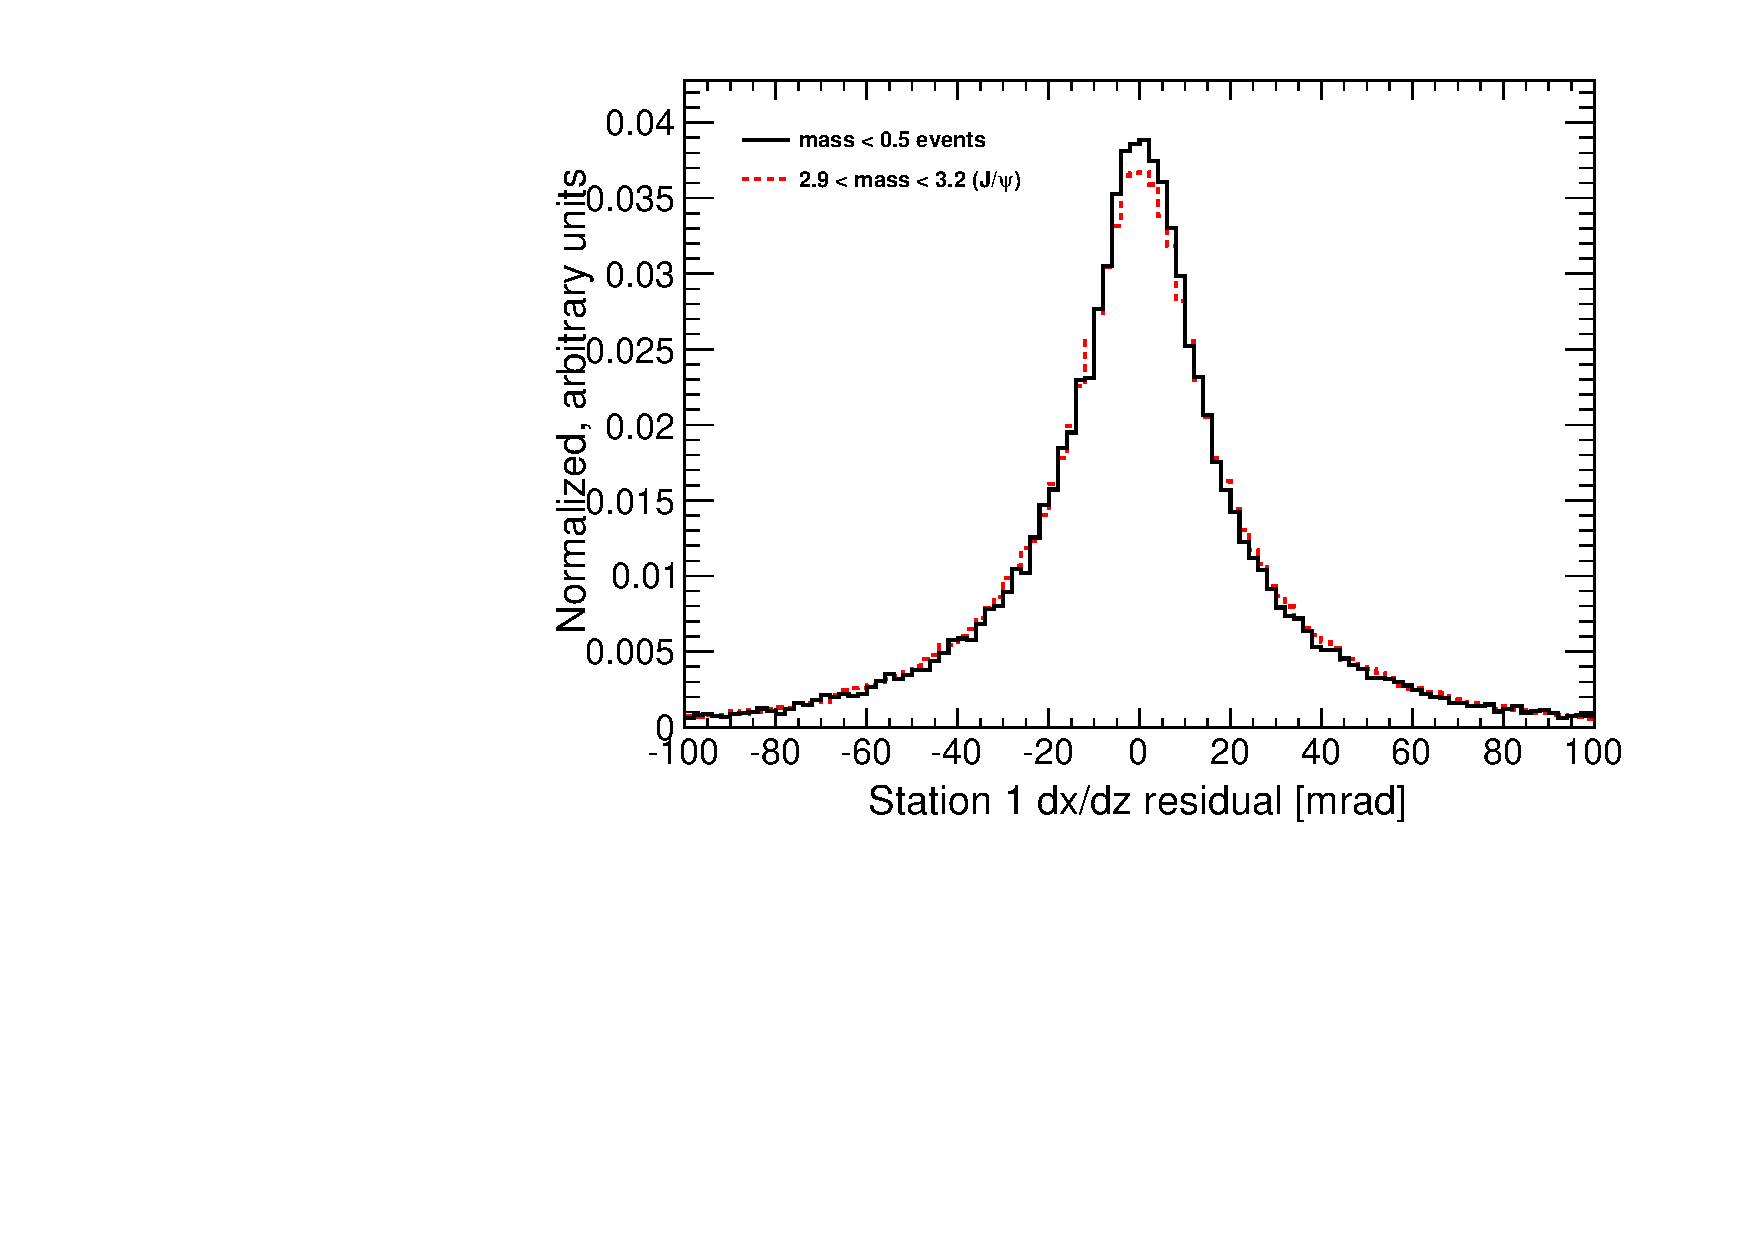
\includegraphics[width=0.45\linewidth]{lowmassquality_st1dxdz.pdf} \hfill
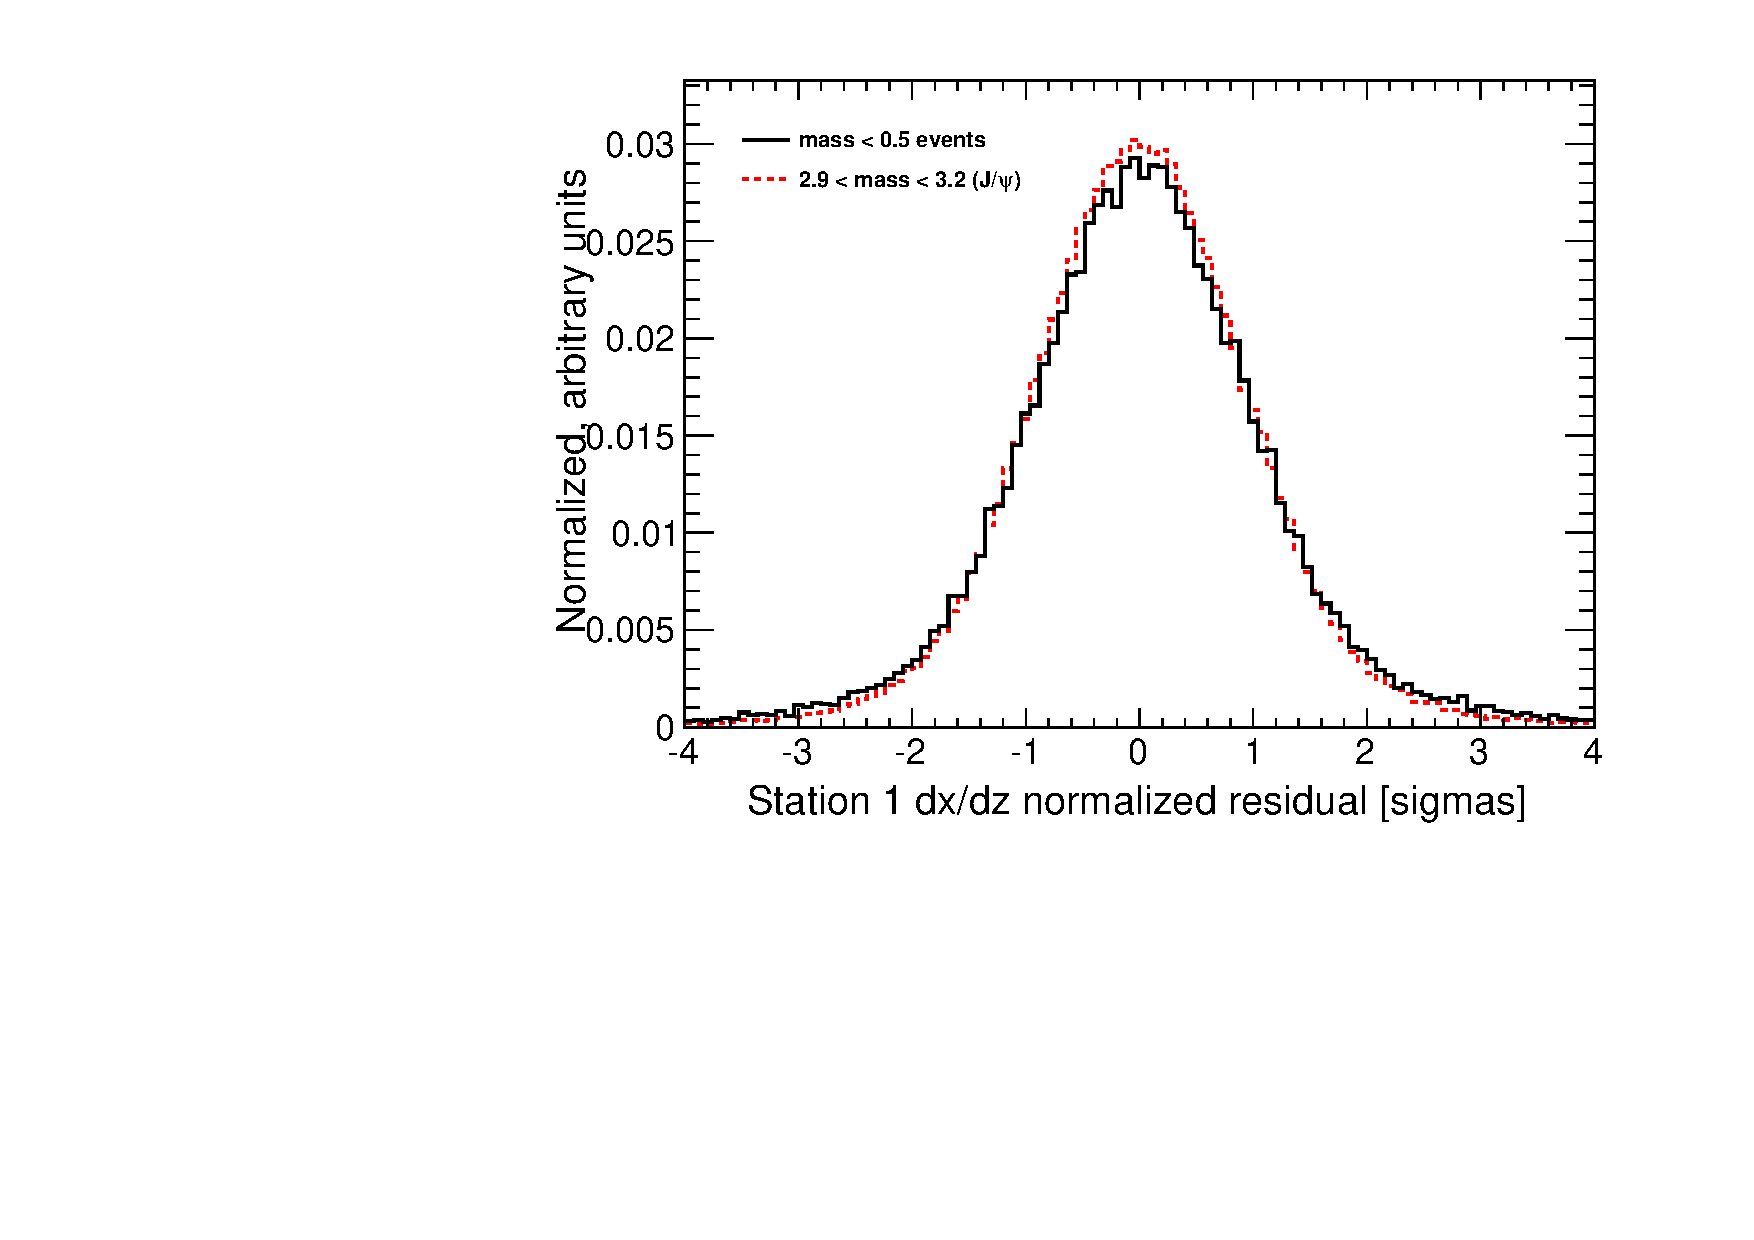
\includegraphics[width=0.45\linewidth]{lowmassquality_st1dxdzsig.pdf}
\end{frame}

\begin{frame}
\frametitle{$p_T$ distributions}
\begin{columns}
\column{0.6\linewidth}
\begin{itemize}
\item Now check dimuon vector-sum $p_T$ distribution of the 1.1 $<$
  mass $<$ 2.9~GeV/$c^2$ region (continuum)
\item Isolated component (below) is not much different from the rest
\end{itemize}

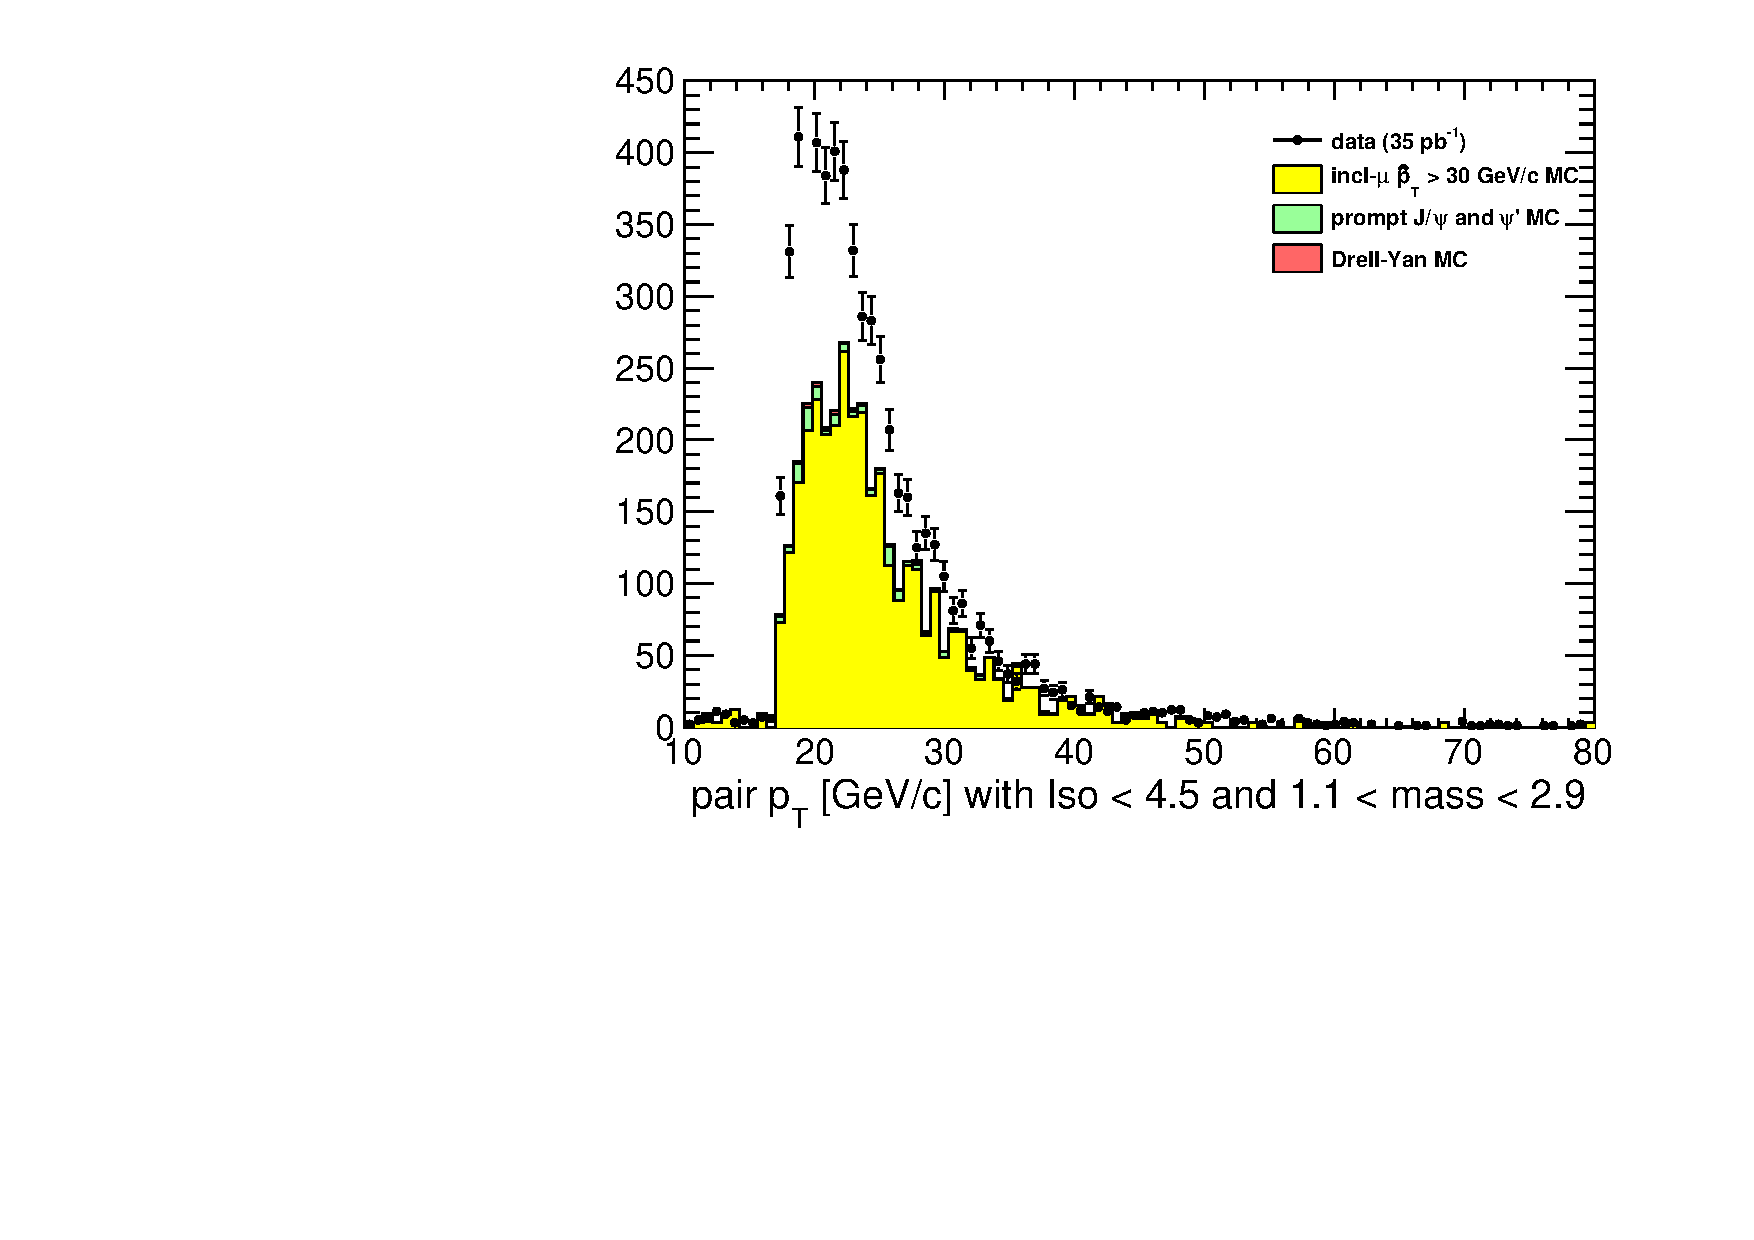
\includegraphics[width=\linewidth]{lowdimuon_pt_midmass_isolated.pdf}

\column{0.4\linewidth}
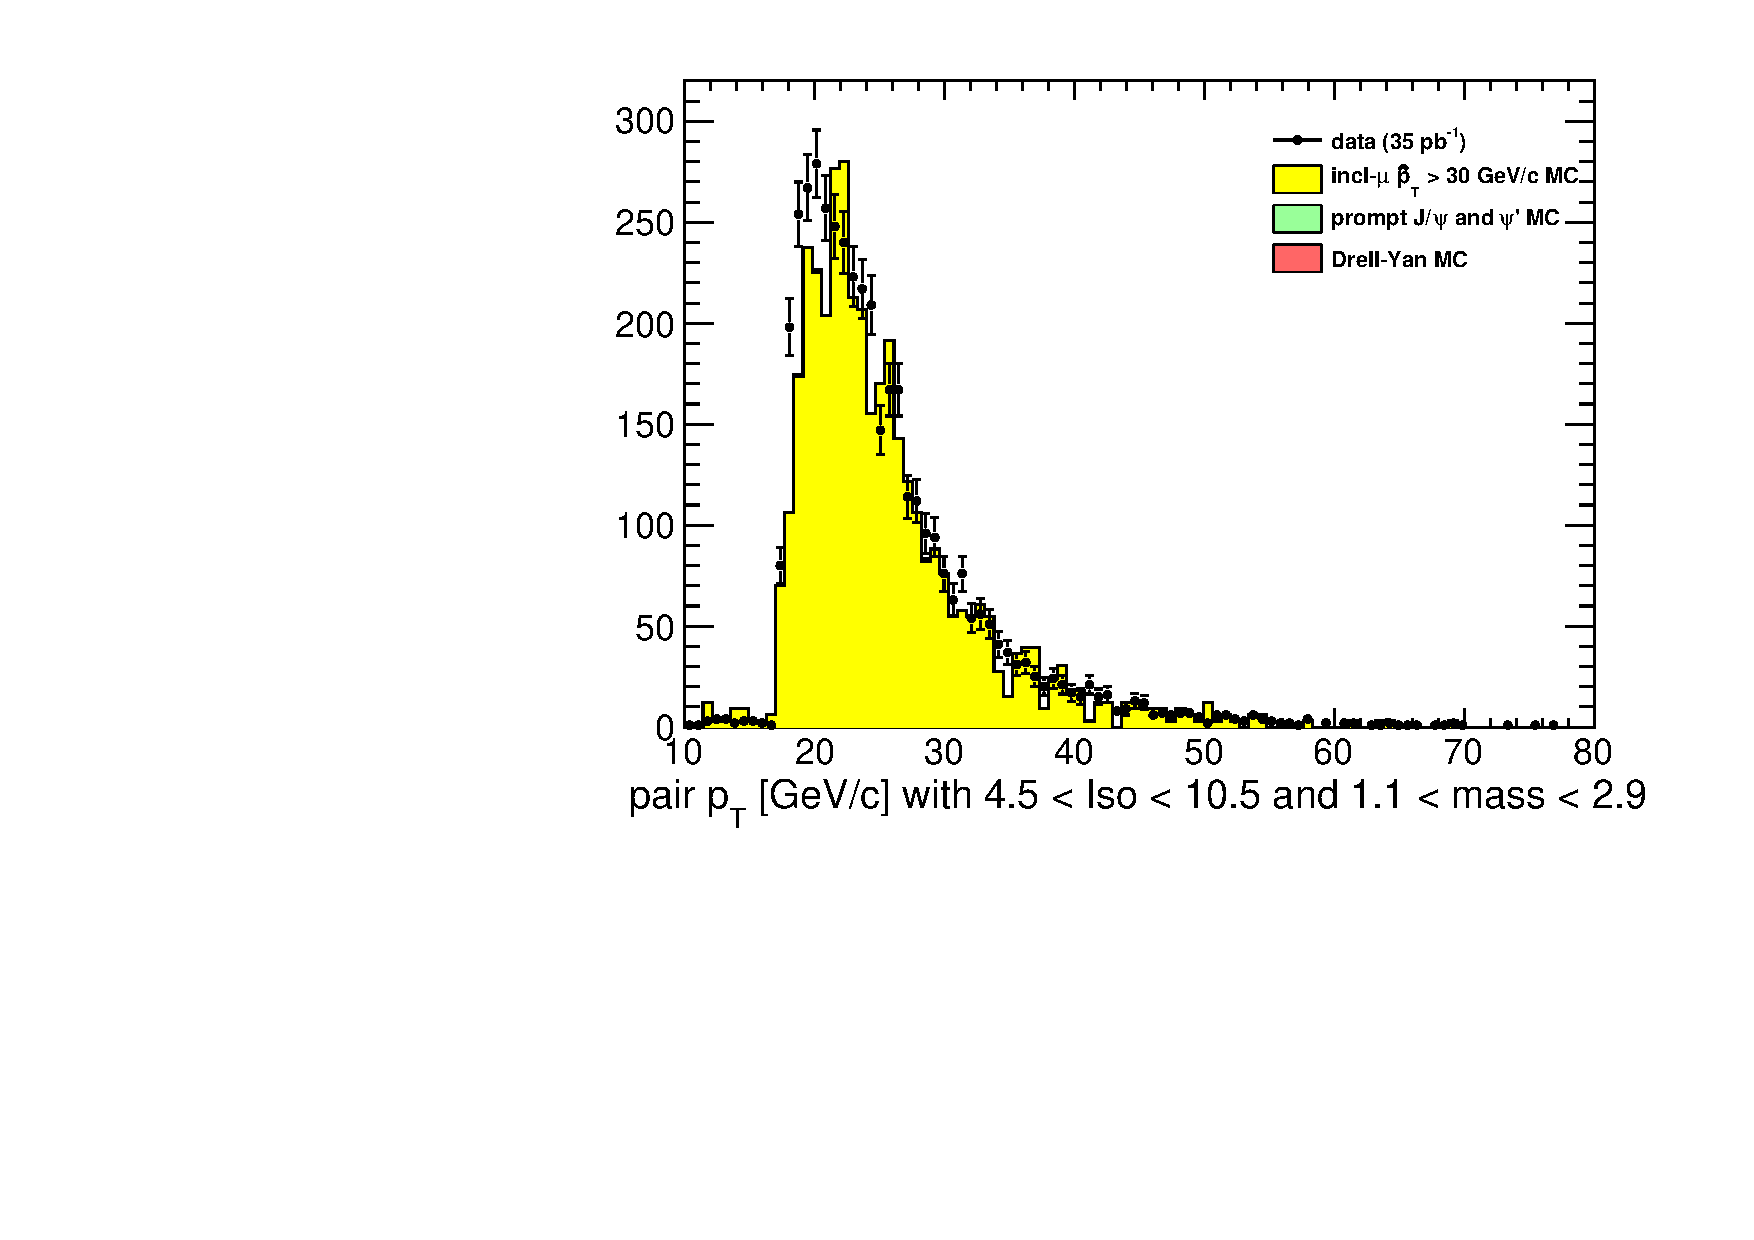
\includegraphics[width=\linewidth]{lowdimuon_pt_midmass_isosideband.pdf}

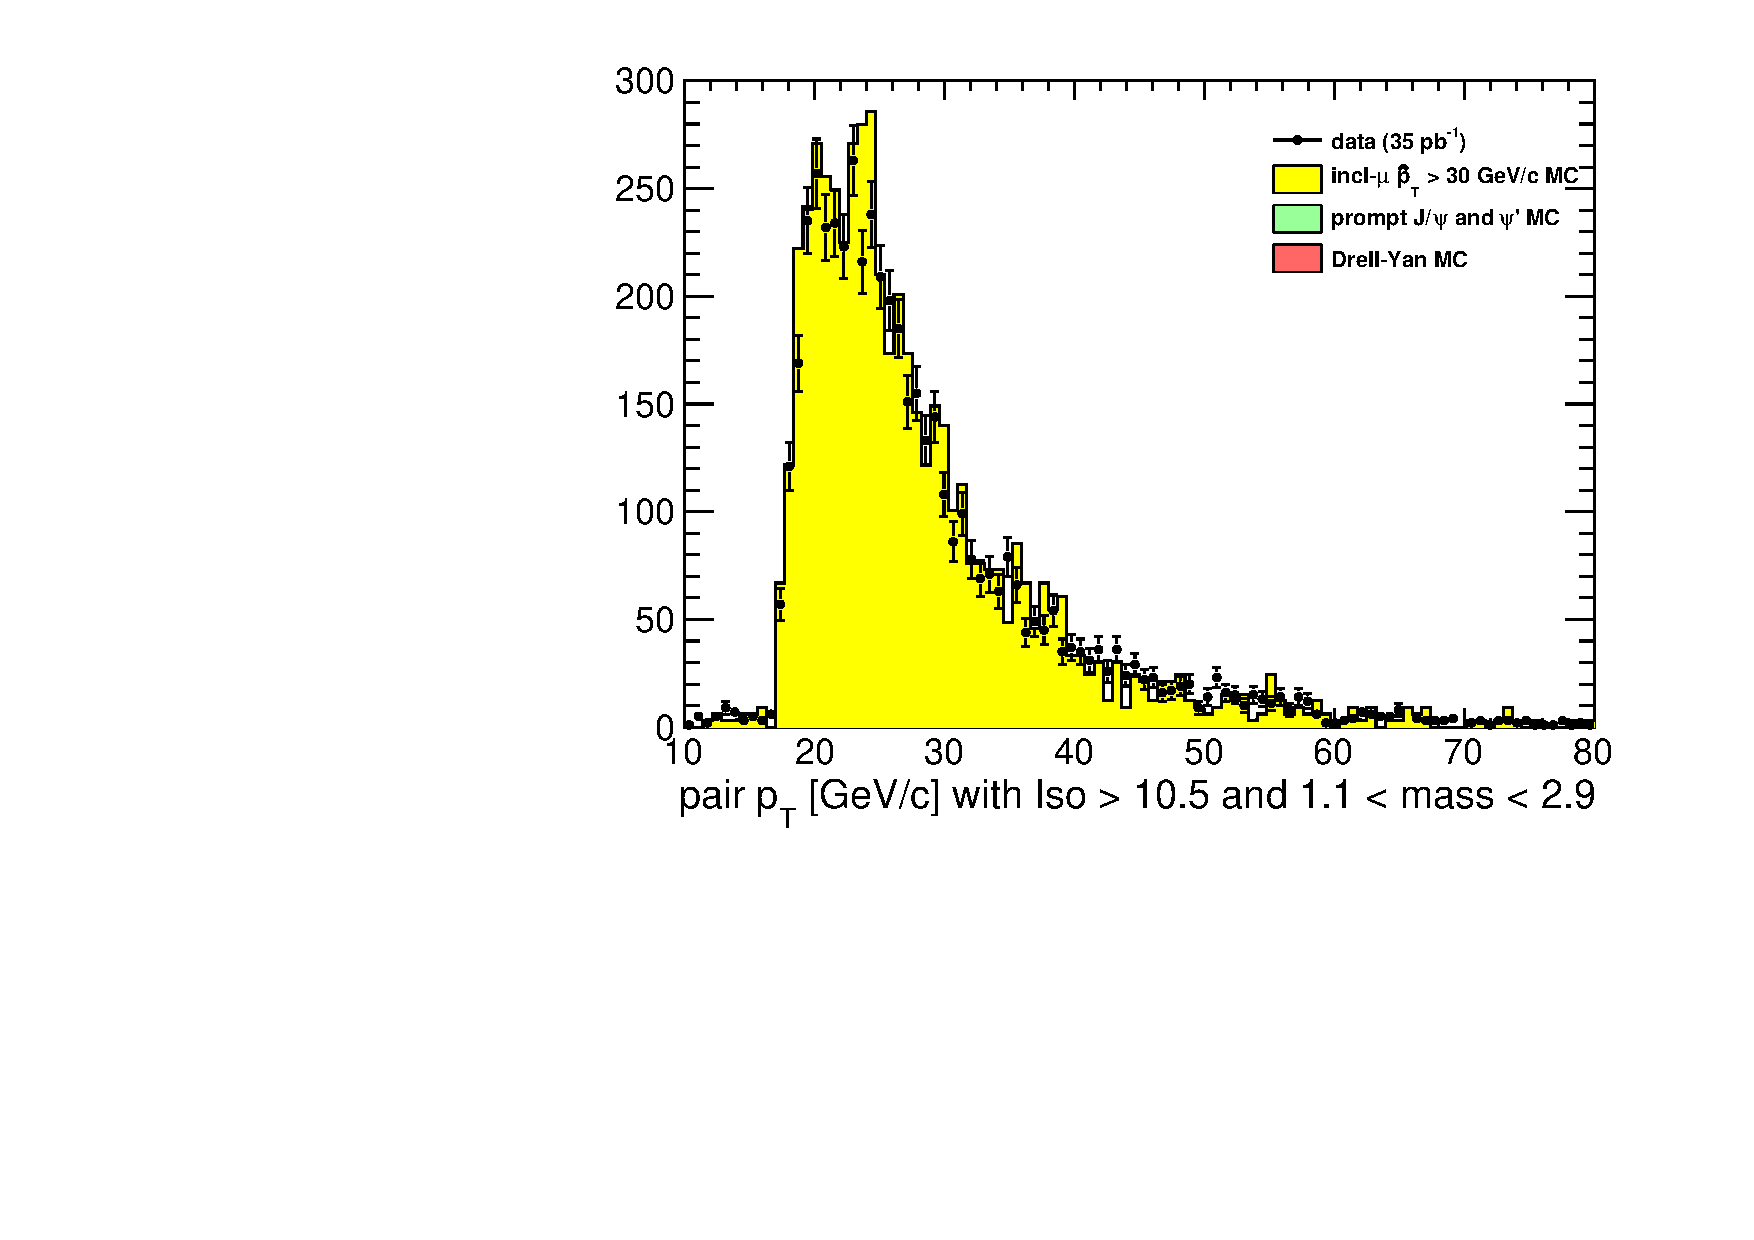
\includegraphics[width=\linewidth]{lowdimuon_pt_midmass_noniso.pdf}
\end{columns}
\end{frame}

\begin{frame}
\frametitle{$p_T$ distributions}
\begin{columns}
\column{0.6\linewidth}
\begin{itemize}
\item Same for mass $<$ 0.5~GeV/$c^2$ region
\end{itemize}

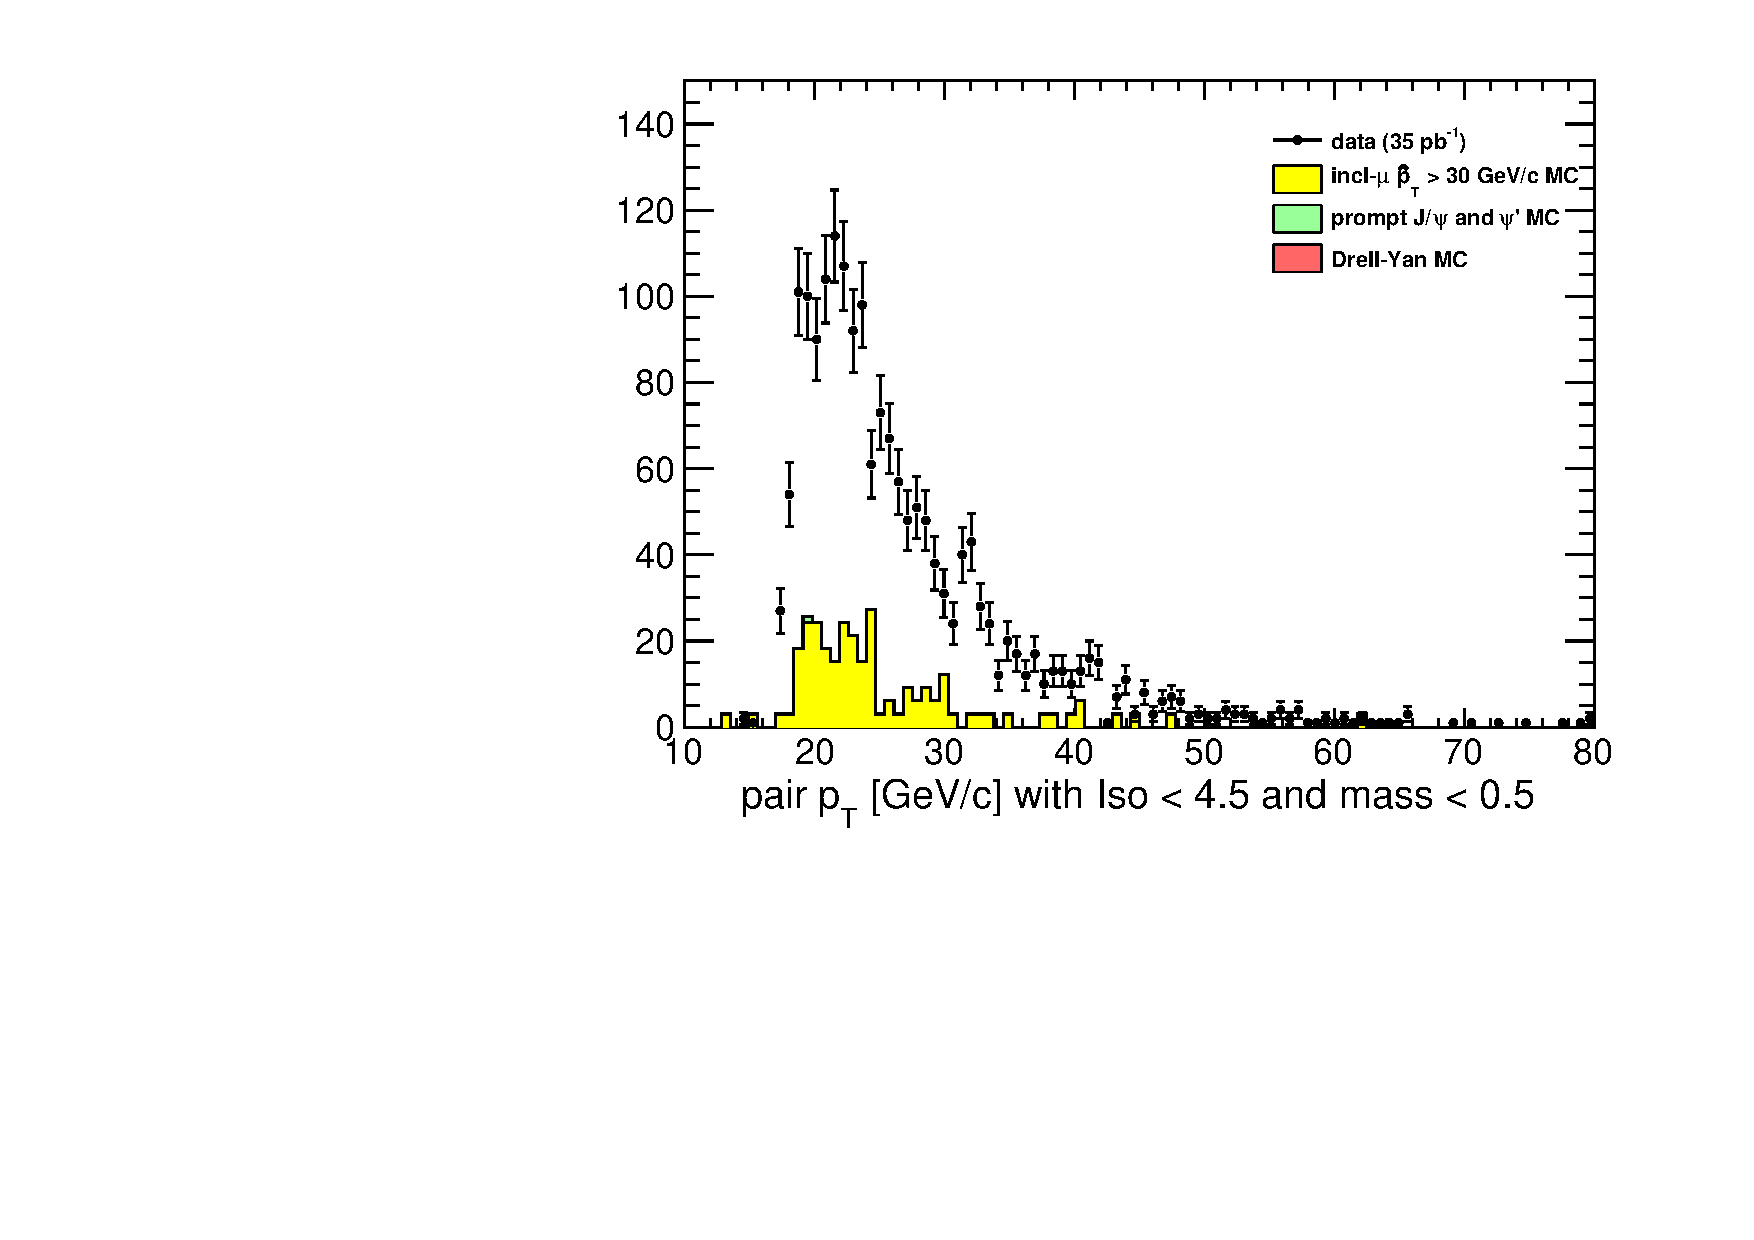
\includegraphics[width=\linewidth]{lowdimuon_pt_lowmass_isolated.pdf}

\column{0.4\linewidth}
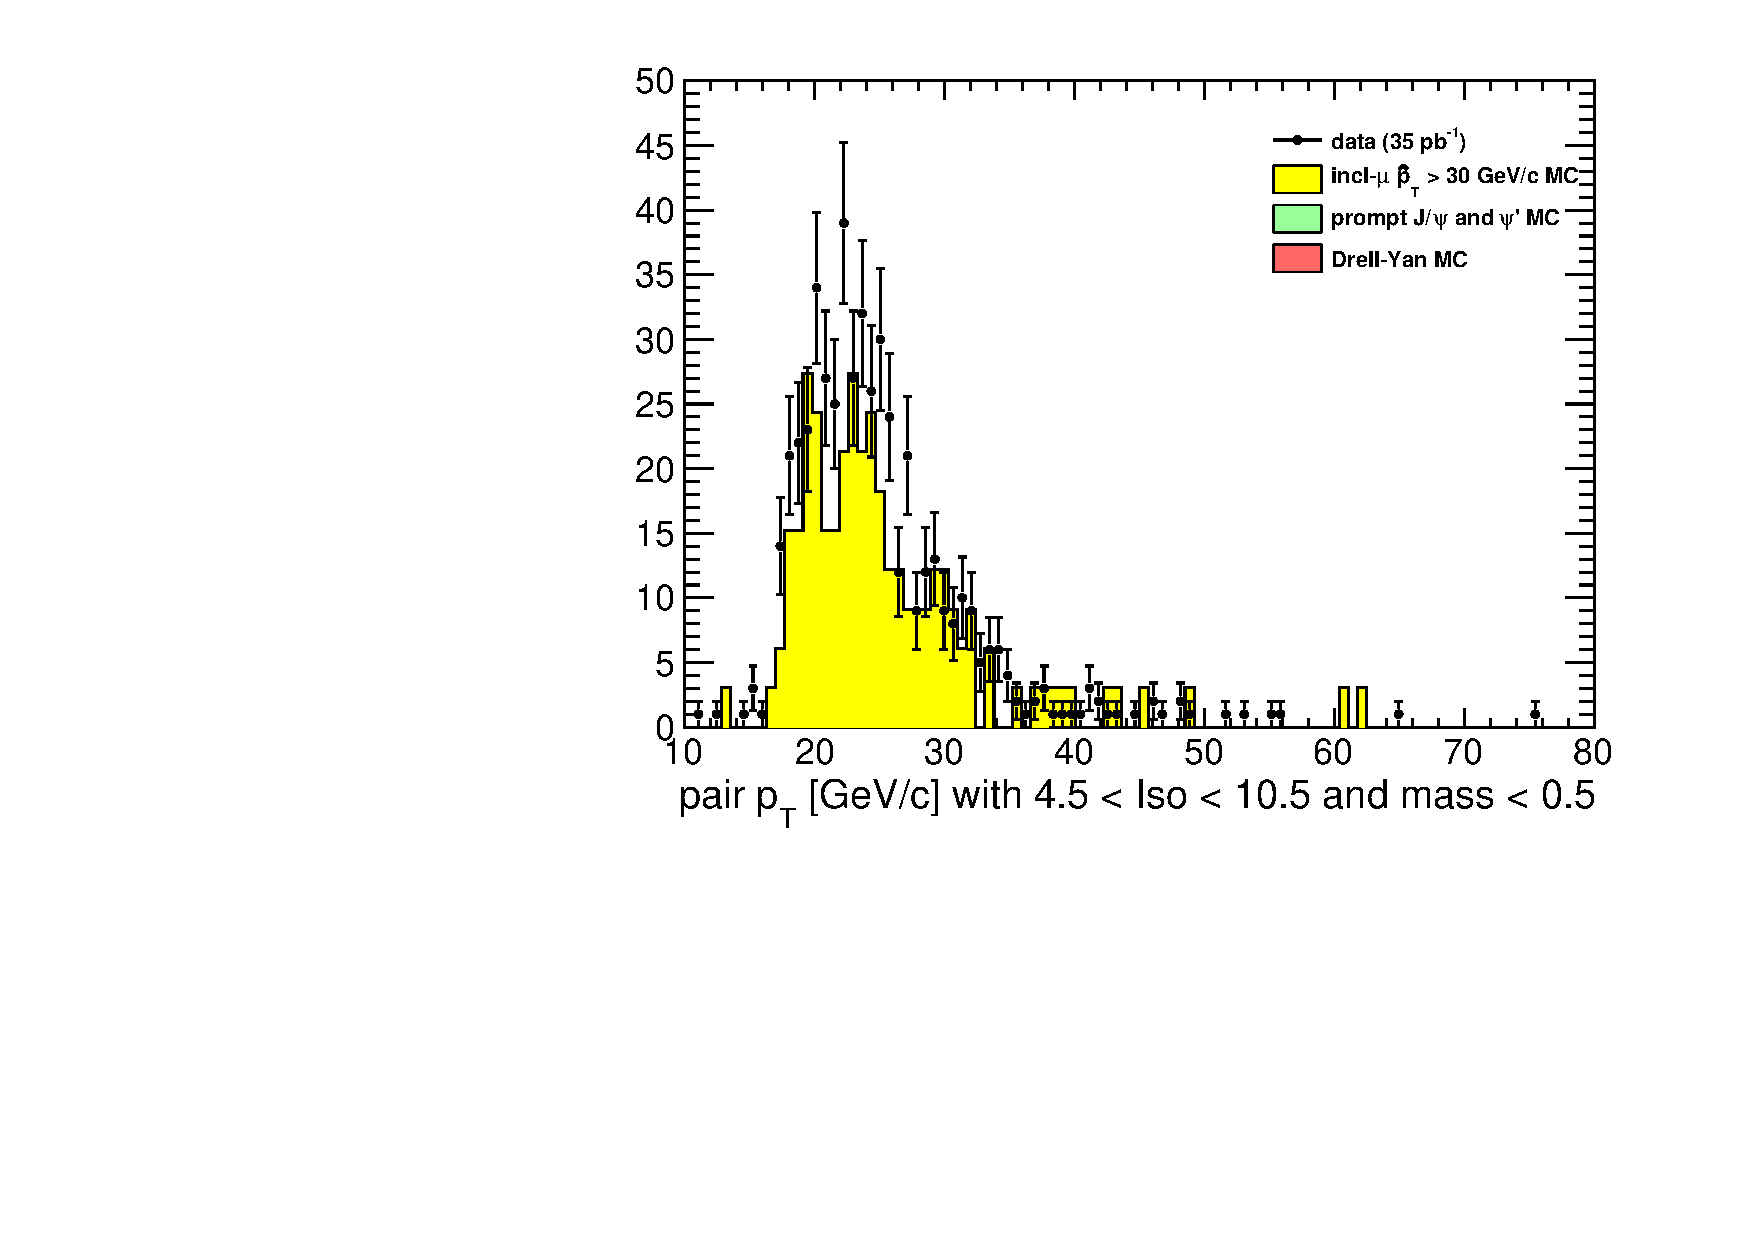
\includegraphics[width=\linewidth]{lowdimuon_pt_lowmass_isosideband.pdf}

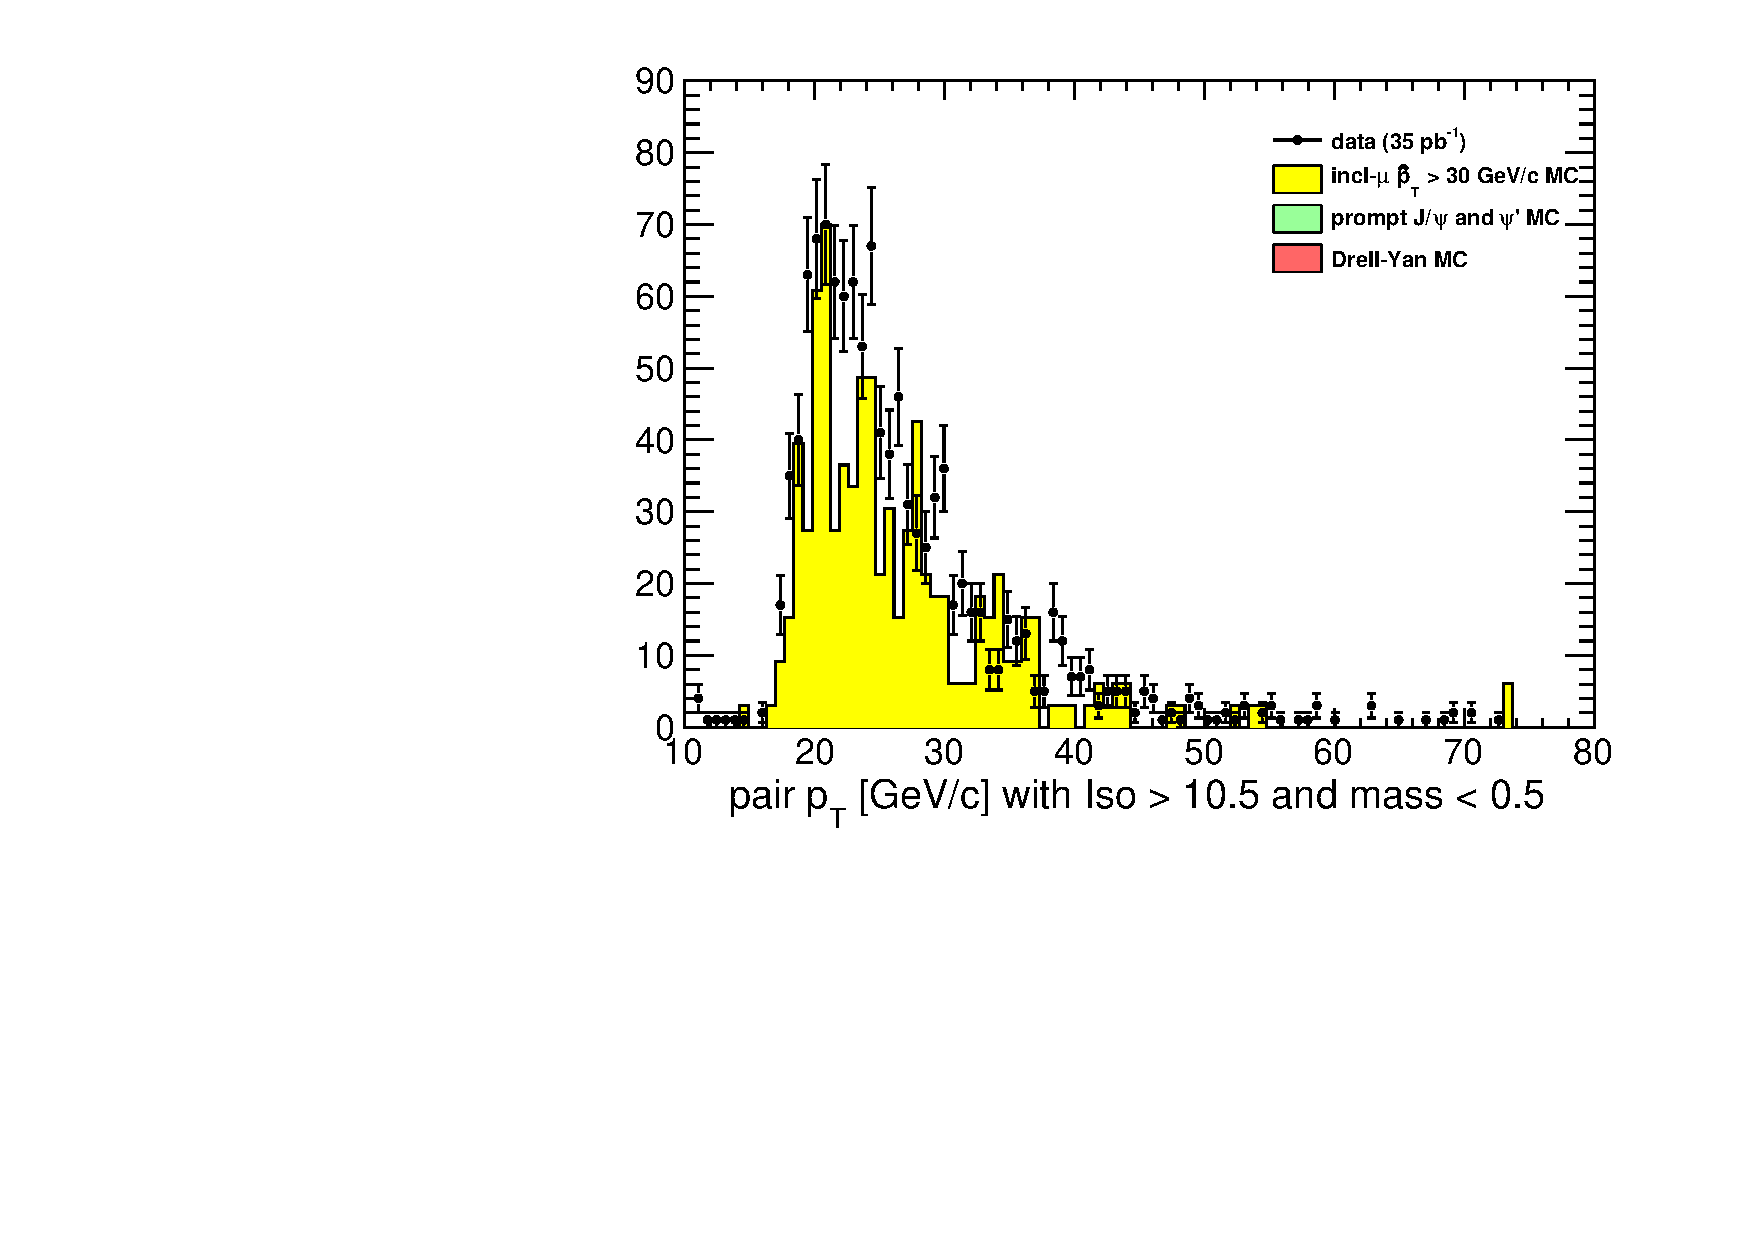
\includegraphics[width=\linewidth]{lowdimuon_pt_lowmass_noniso.pdf}
\end{columns}
\end{frame}

\begin{frame}
\frametitle{Other variables}
\begin{columns}
\column{0.6\linewidth}
\begin{itemize}
\item This is the 1.1 $<$ mass $<$ 2.9~GeV/$c^2$ region (continuum) in
  $P_\s{vertex}$, $\phi$, $\eta$
\item Studying only the isolated component
\item $b\bar{b}$ has poor $P_\s{vertex}$ because the two muons
  sometimes come from different decays
\end{itemize}

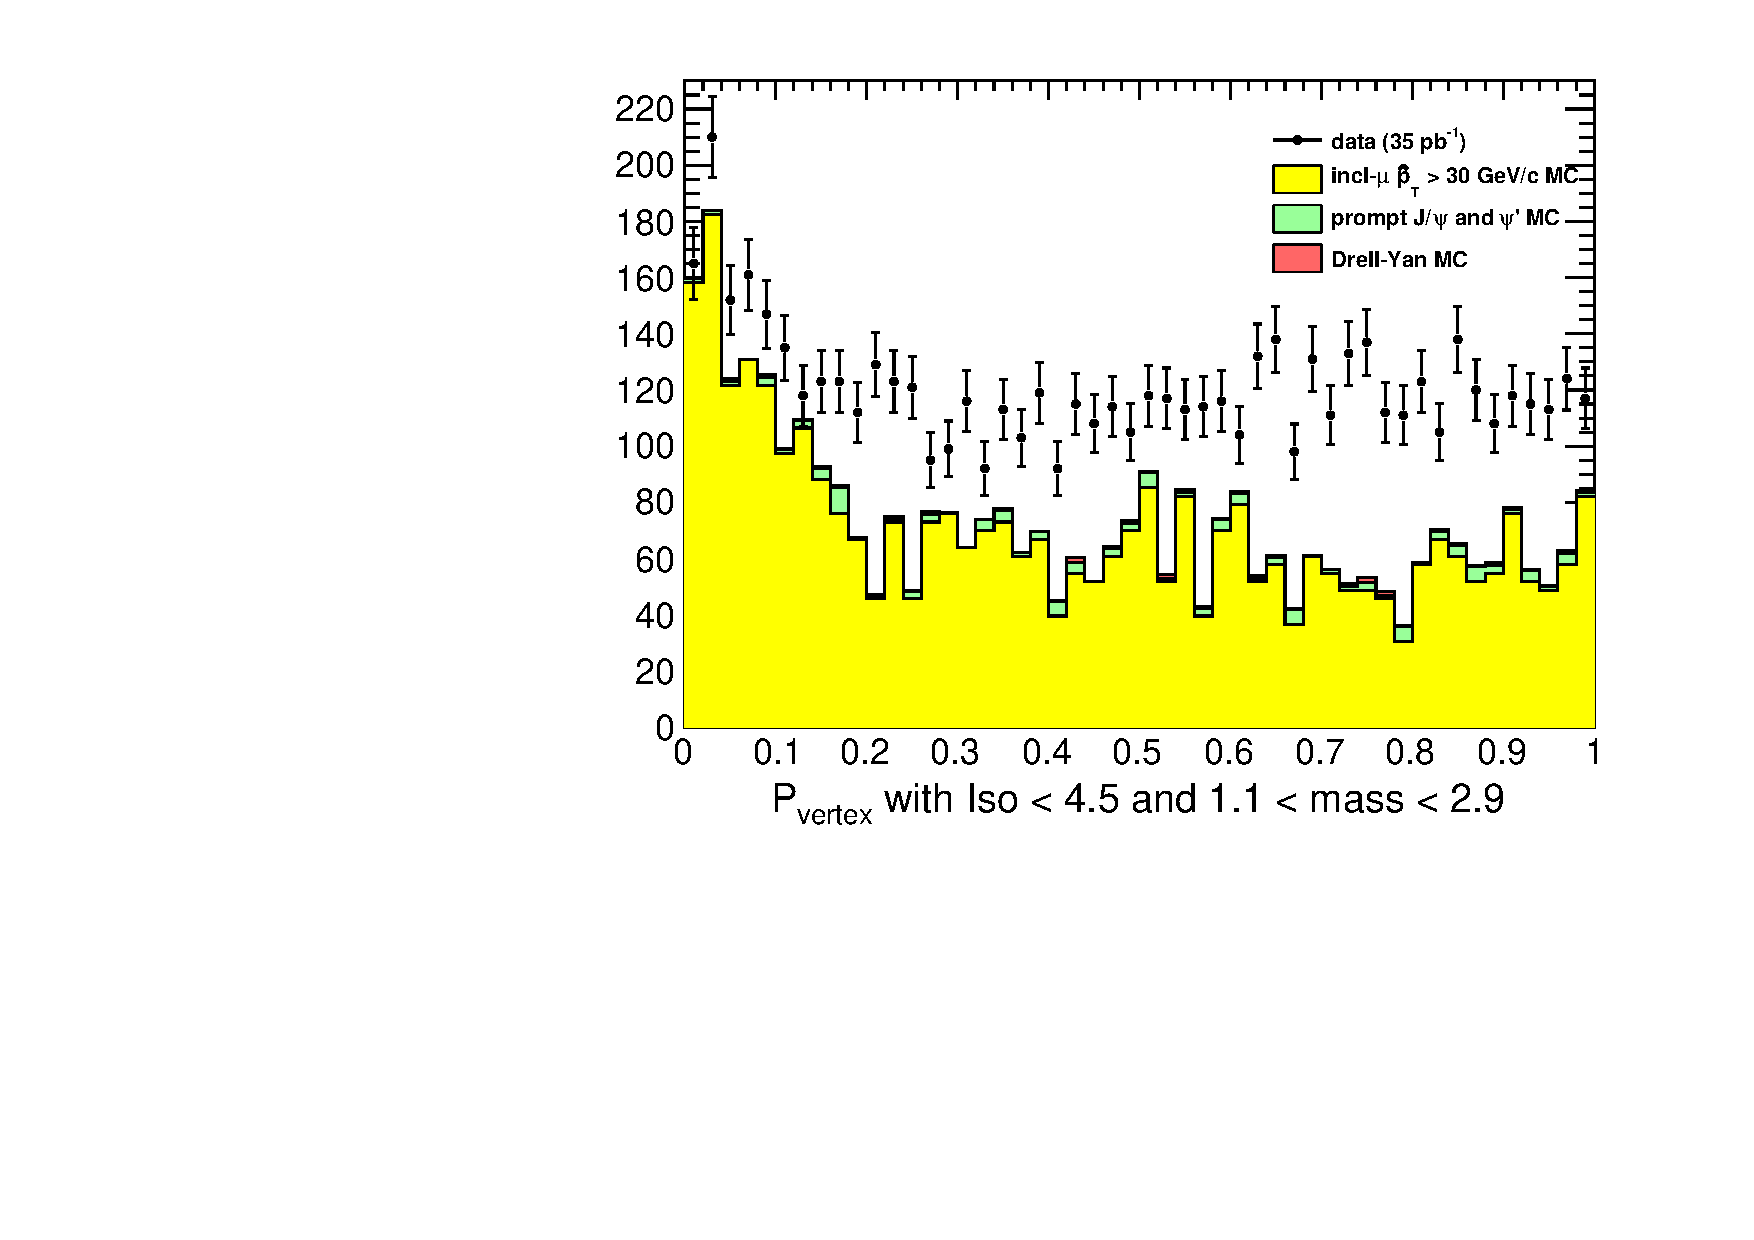
\includegraphics[width=\linewidth]{lowdimuon_vprob_midmass_isolated.pdf}

\column{0.4\linewidth}
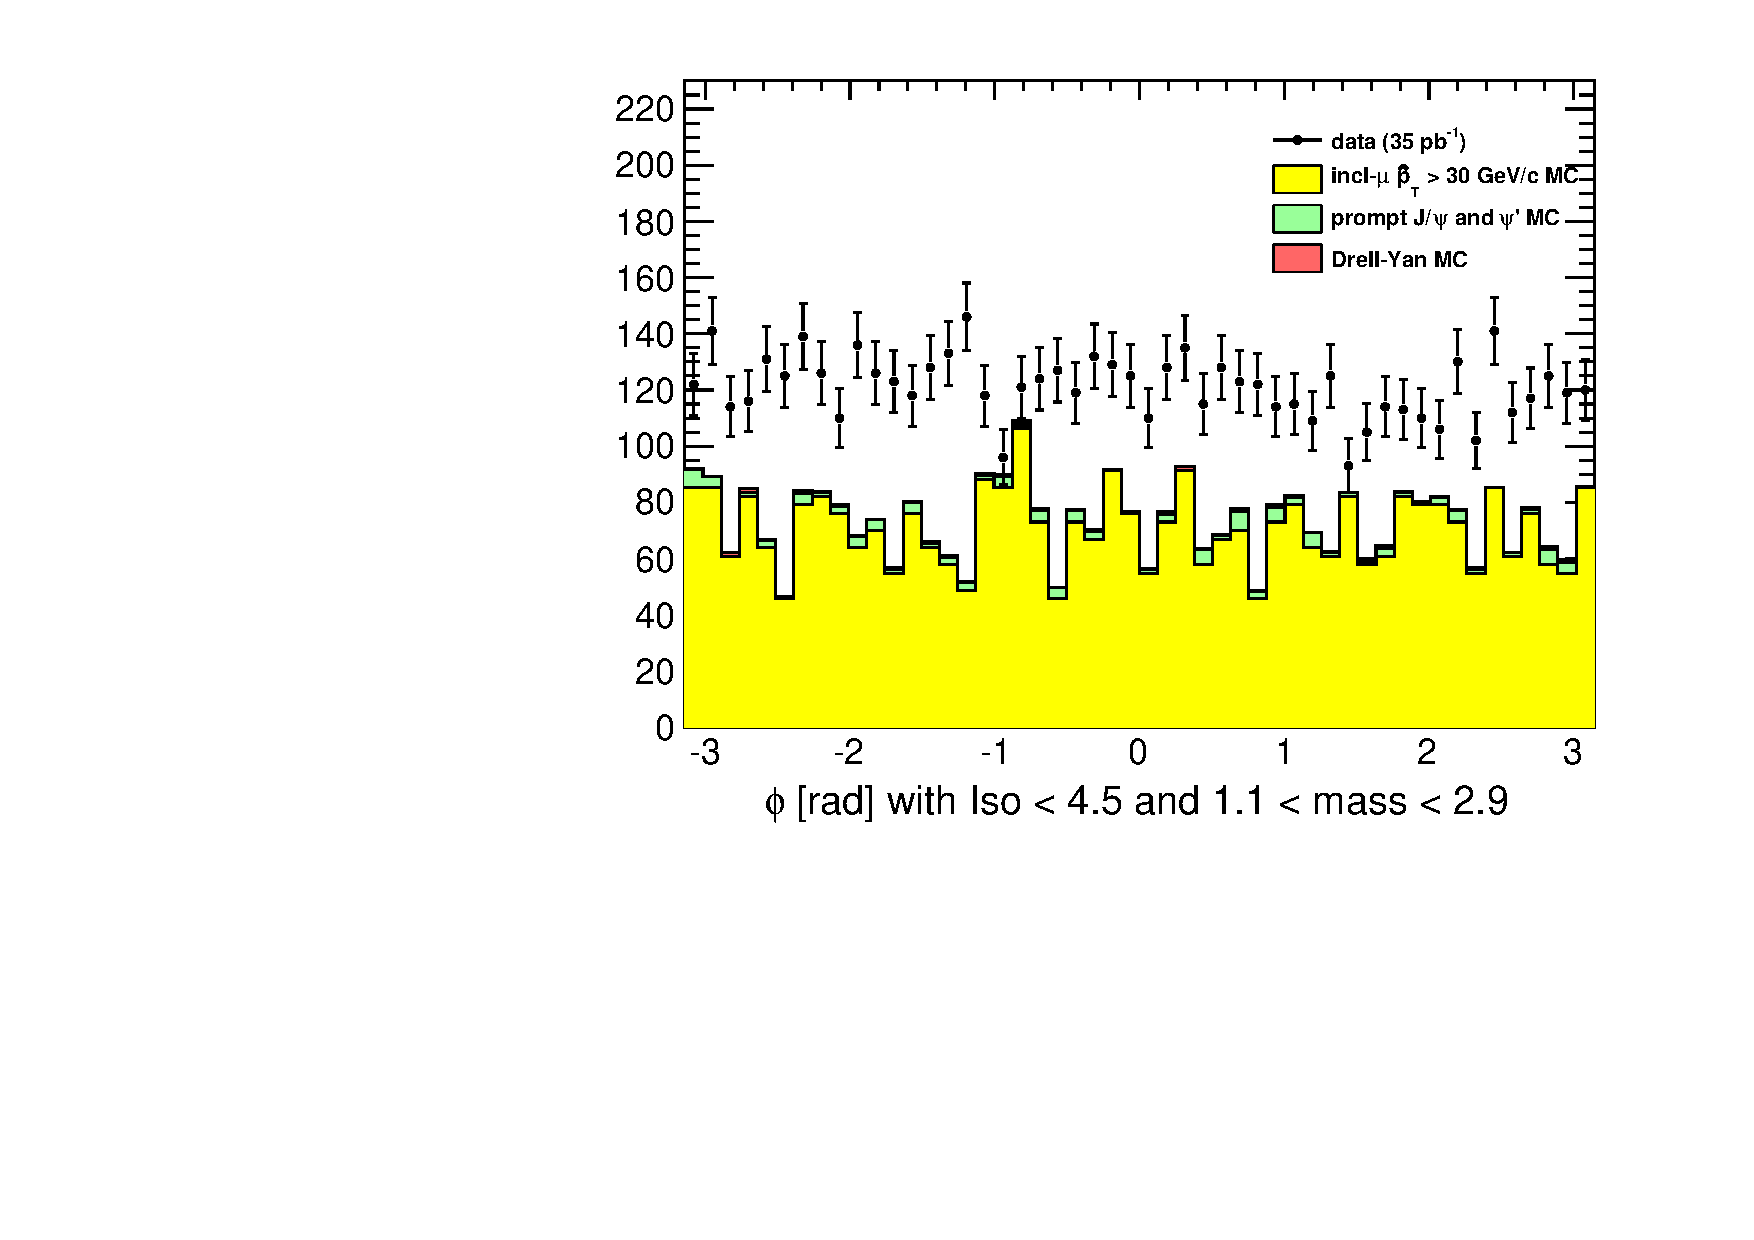
\includegraphics[width=\linewidth]{lowdimuon_phi_midmass_isolated.pdf}

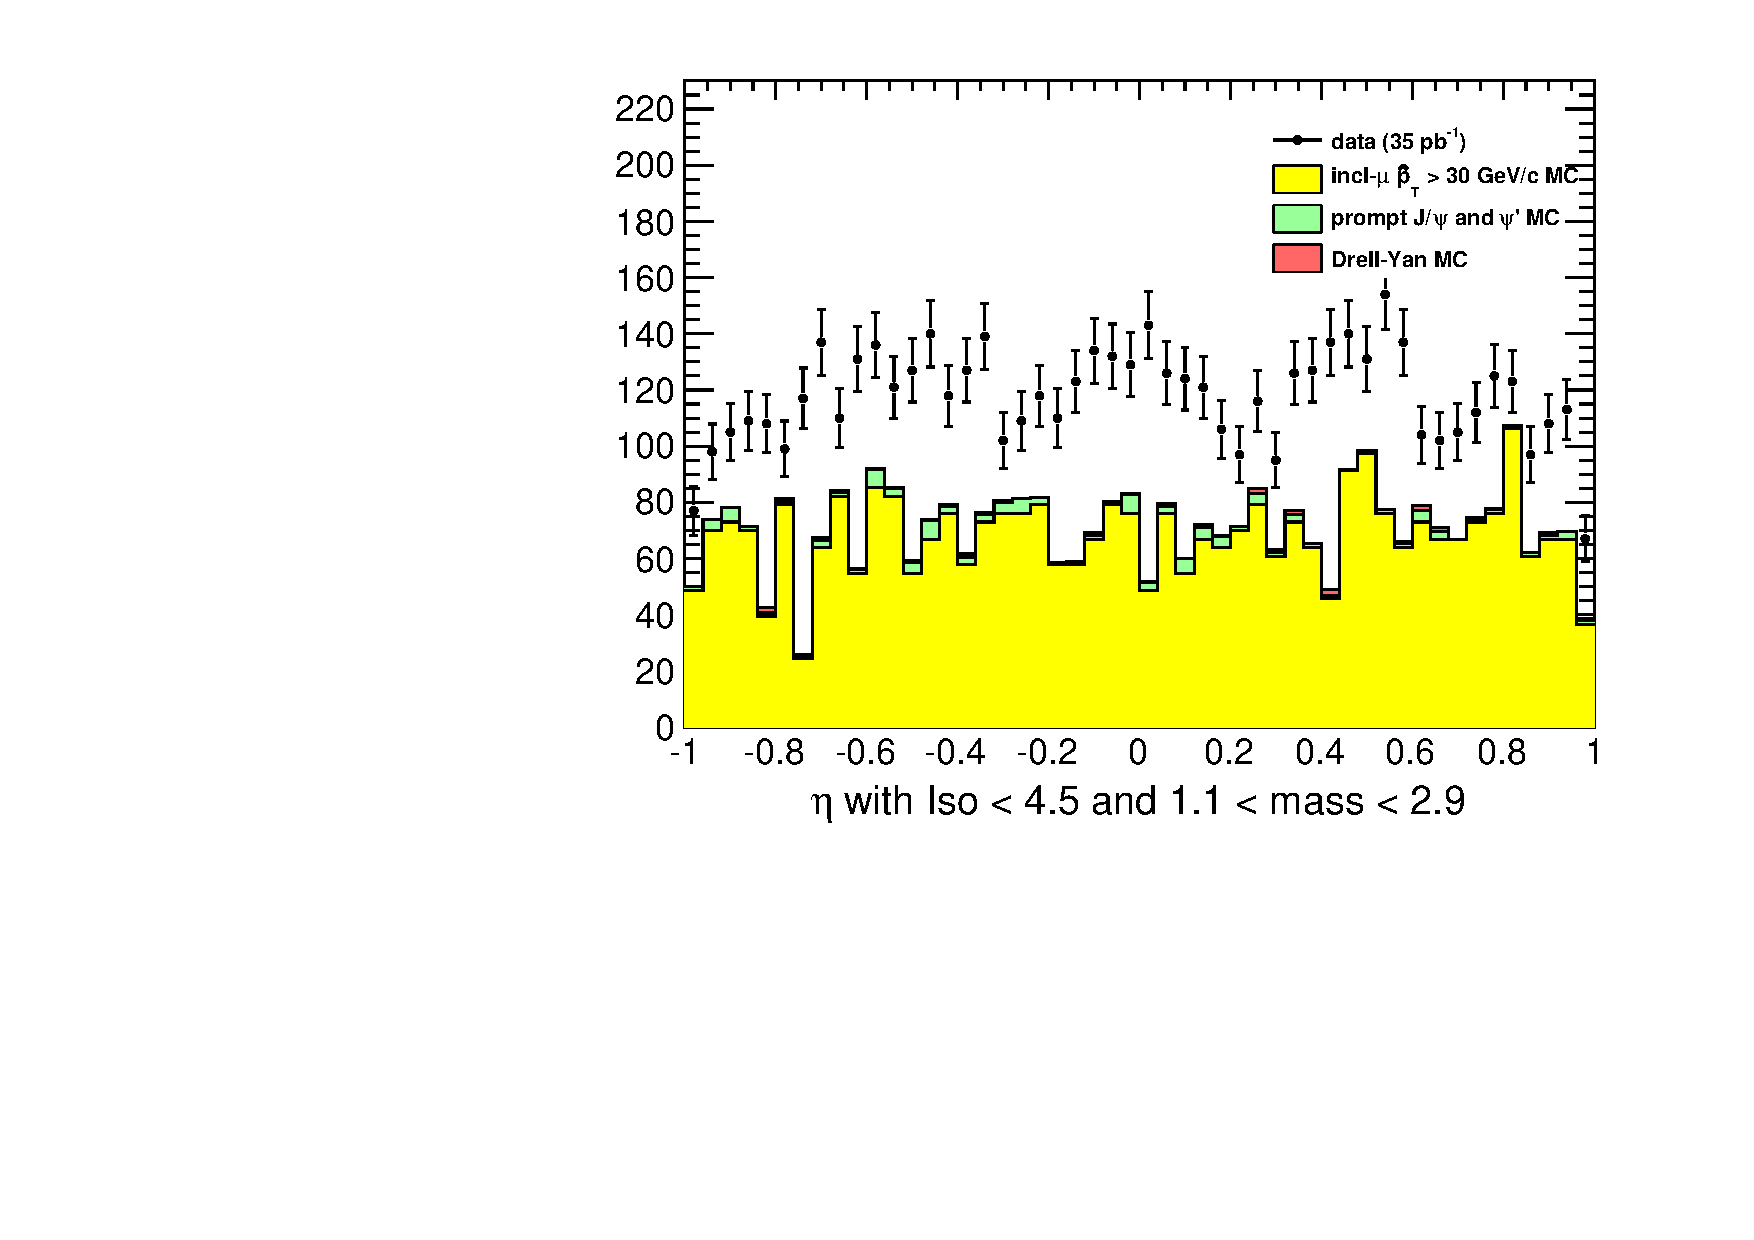
\includegraphics[width=\linewidth]{lowdimuon_eta_midmass_isolated.pdf}
\end{columns}
\end{frame}

\begin{frame}
\frametitle{Other variables}
\begin{columns}
\column{0.6\linewidth}
\begin{itemize}
\item This is the mass $<$ 0.5~GeV/$c^2$ region in
  $P_\s{vertex}$, $\phi$, $\eta$
\item Studying only the isolated component
\item These very small opening angles apparently have a bias toward
  high $P_\s{vertex}$ (errors are underestimated)

(same for continuum: see prev page)
\end{itemize}

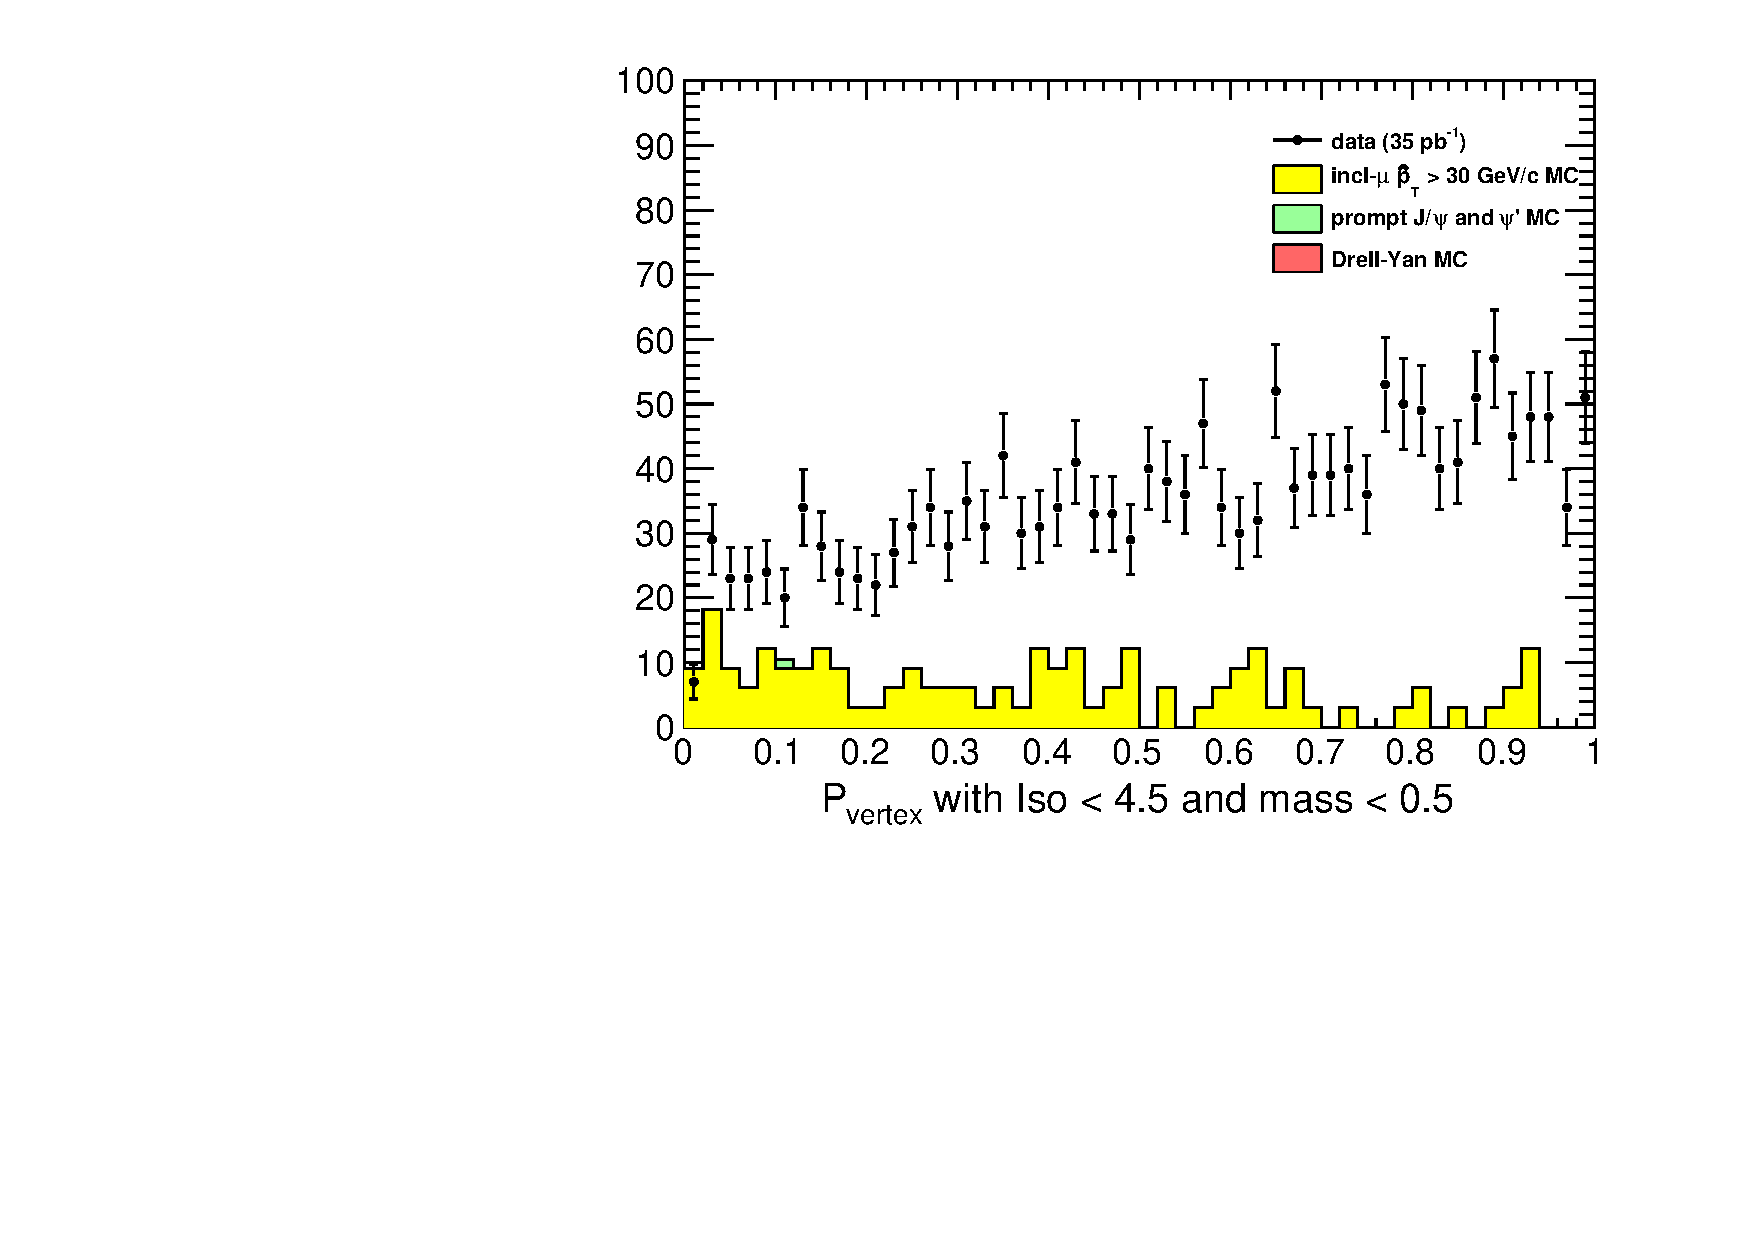
\includegraphics[width=\linewidth]{lowdimuon_vprob_lowmass_isolated.pdf}

\column{0.4\linewidth}
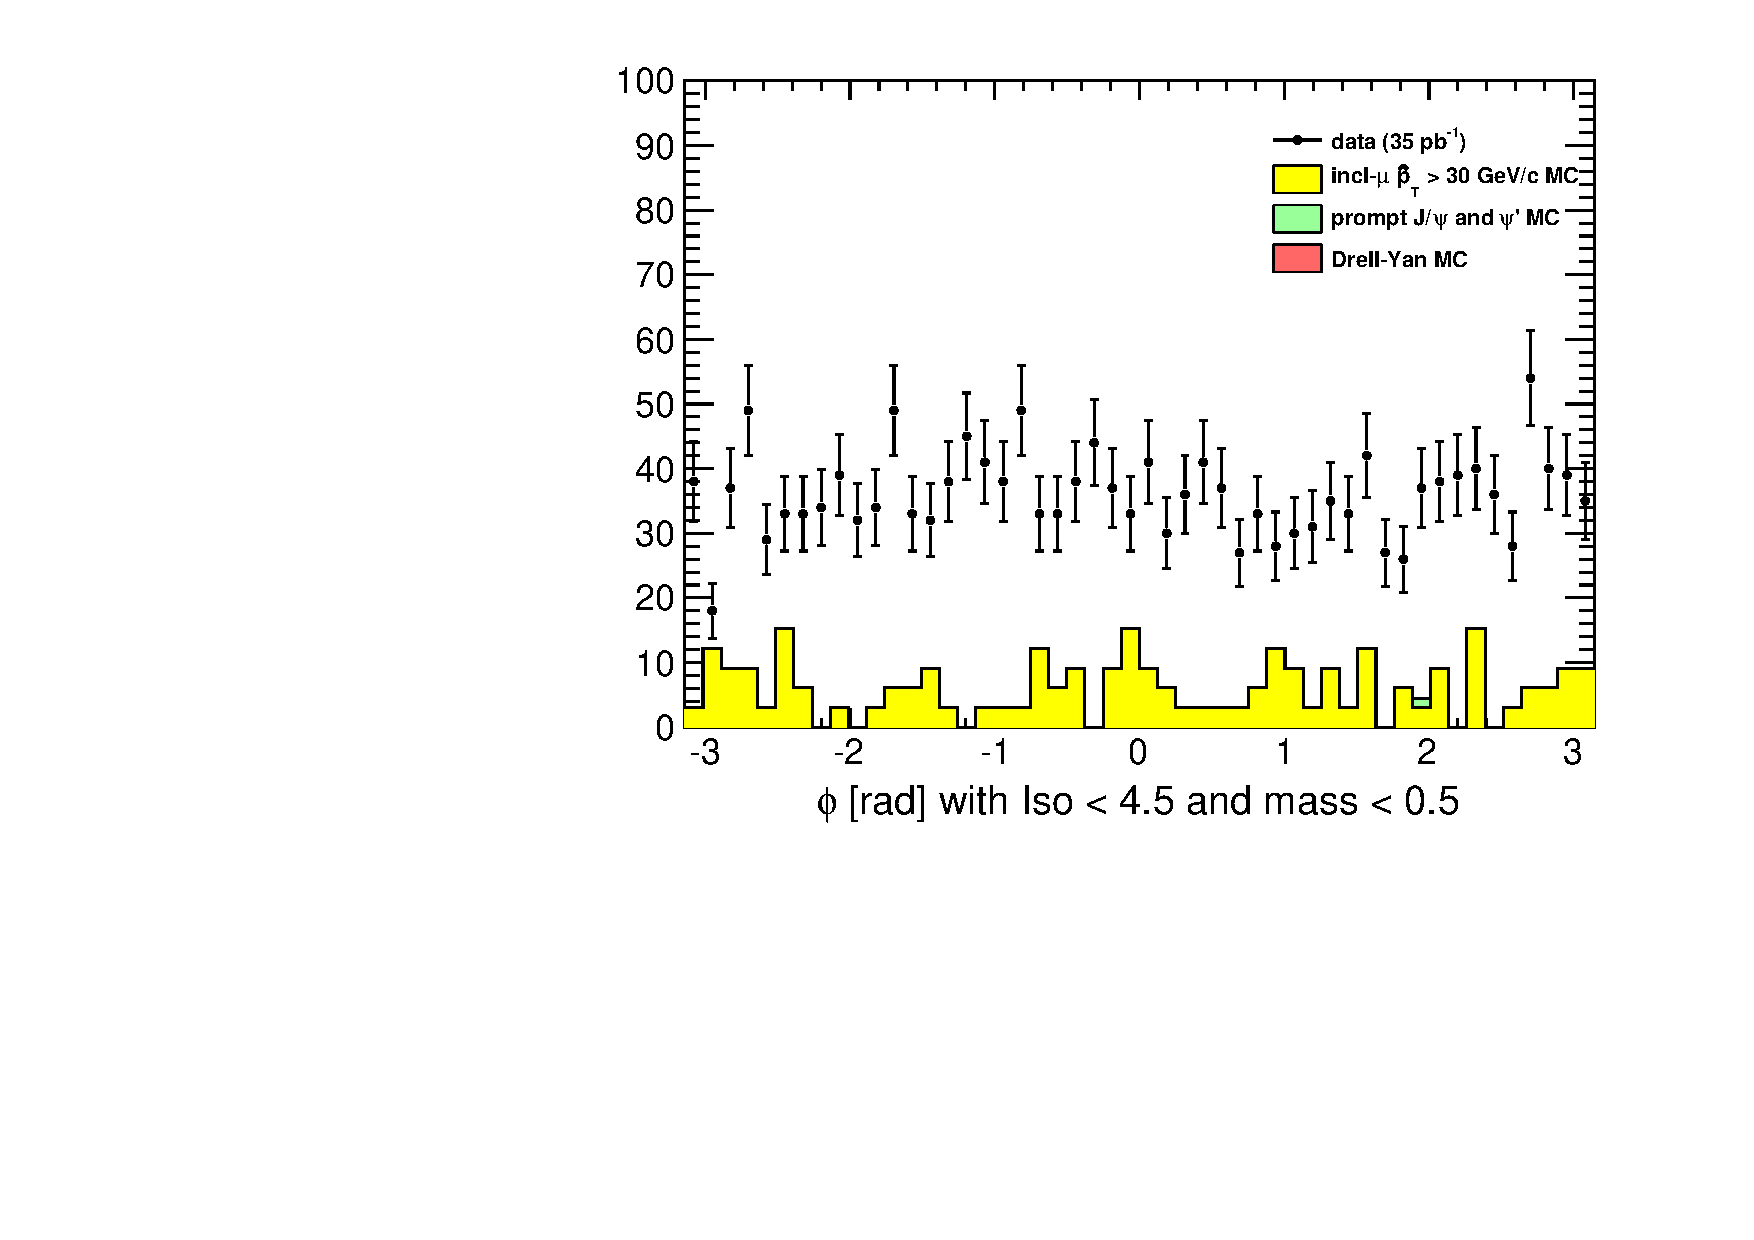
\includegraphics[width=\linewidth]{lowdimuon_phi_lowmass_isolated.pdf}

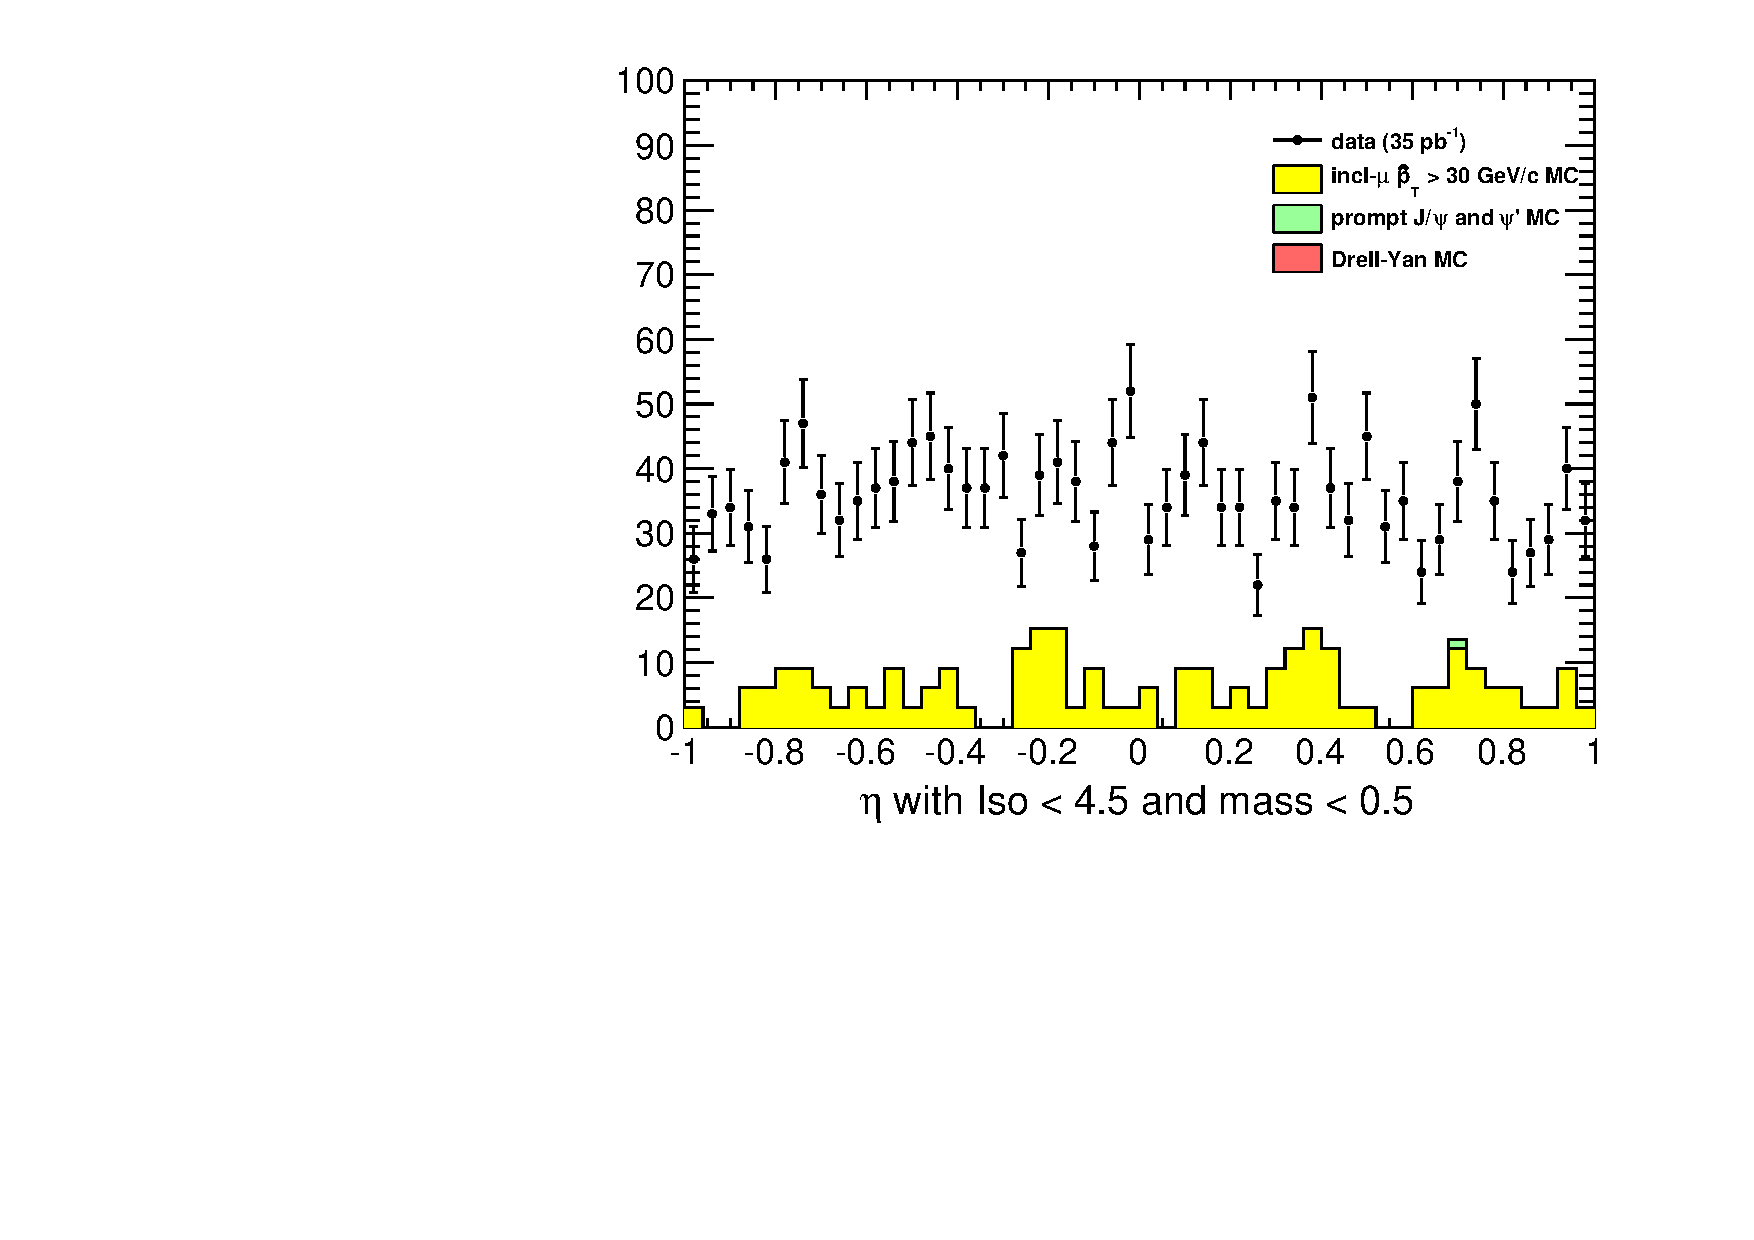
\includegraphics[width=\linewidth]{lowdimuon_eta_lowmass_isolated.pdf}
\end{columns}
\end{frame}

\begin{frame}
\frametitle{Flight significance}

\begin{columns}
\column{0.6\linewidth}
\begin{itemize}
\item This is the 1.1 $<$ mass $<$ 2.9~GeV/$c^2$ (continuum) in
  $L_{xyz} = \vec{x} \cdot \vec{p} / |\vec{p}|$ where $\vec{x}$ is the
  displacement between the dimuon vertex and the closest primary
  vertex in $z$

\item Left edge (wrong-direction flights) is resolution; right tail is $\gamma c \tau$

\item Beampipe is at 30~mm
\end{itemize}

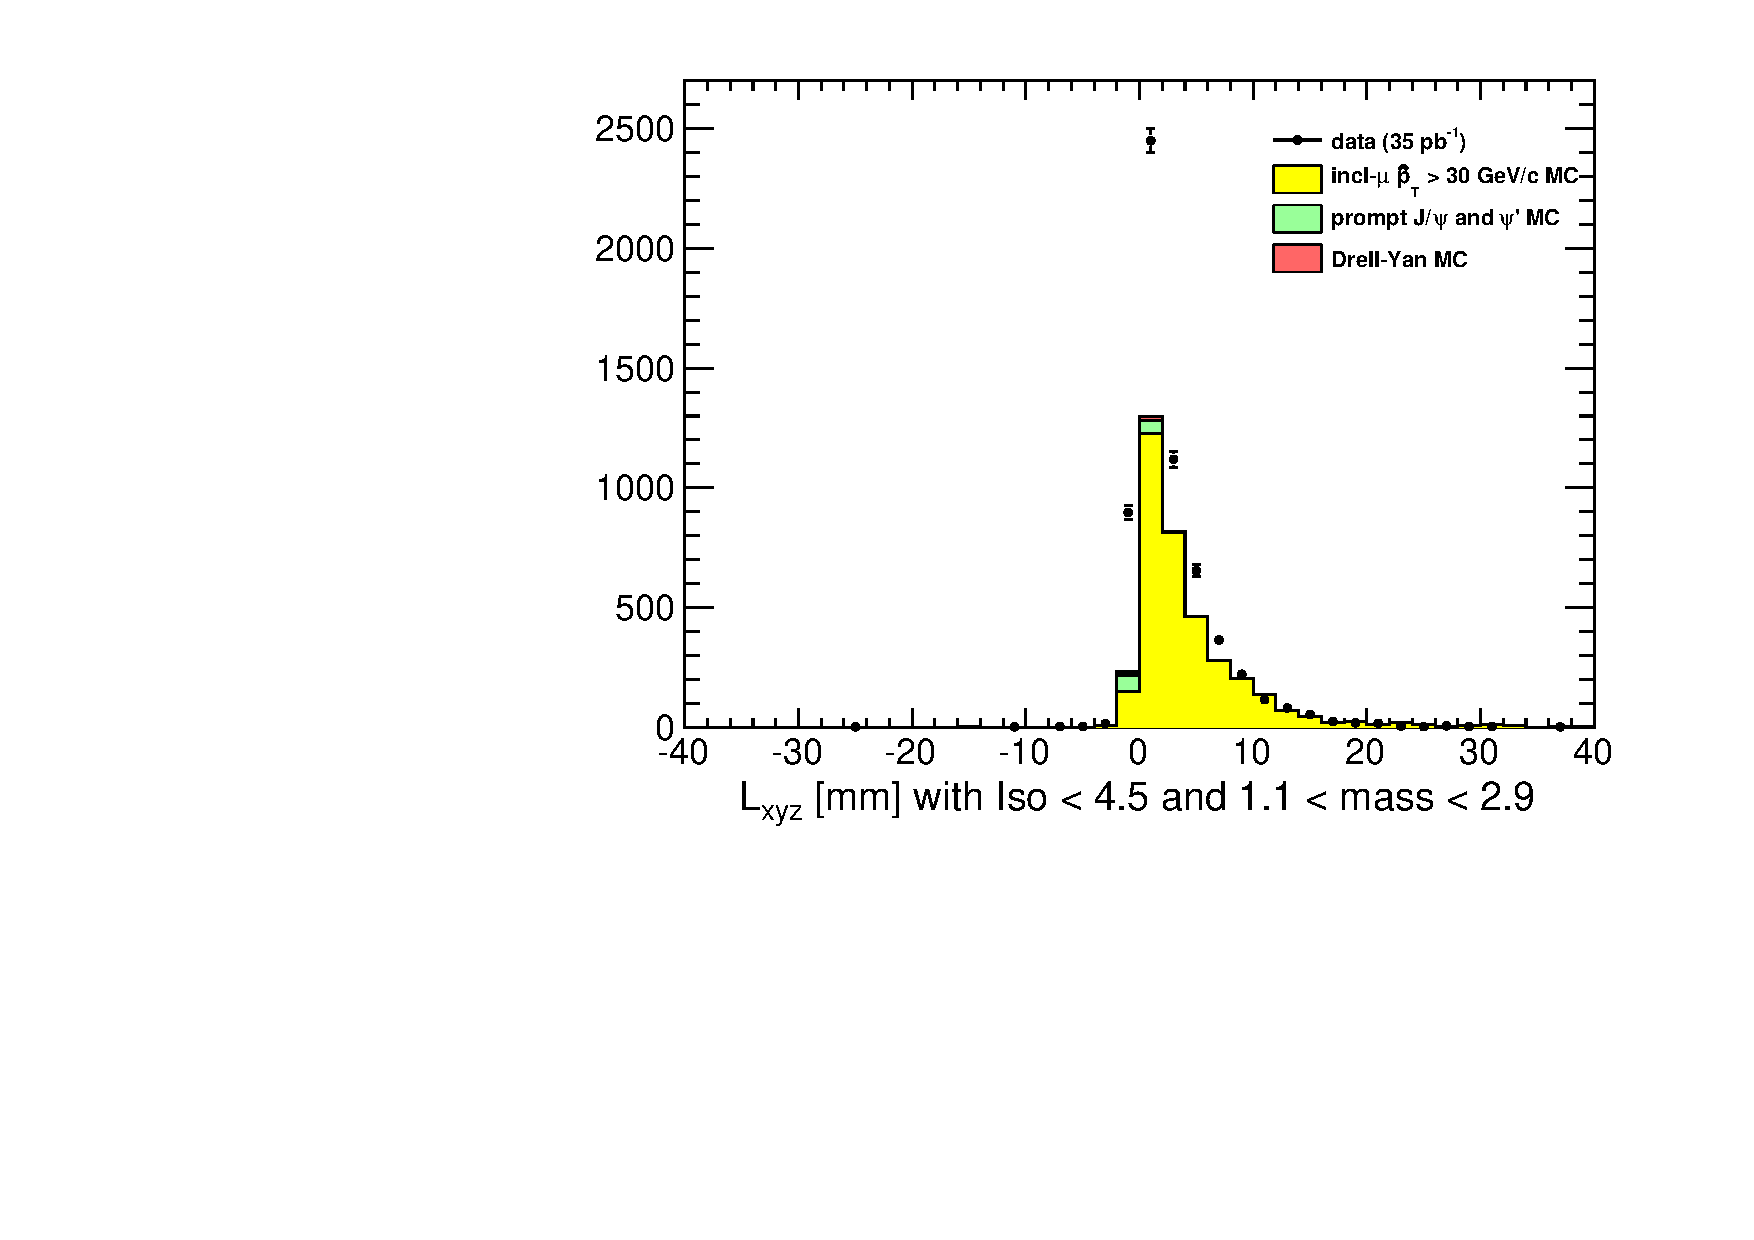
\includegraphics[width=\linewidth]{lowdimuon_lxyz_midmass_isolated.pdf}

\column{0.4\linewidth}
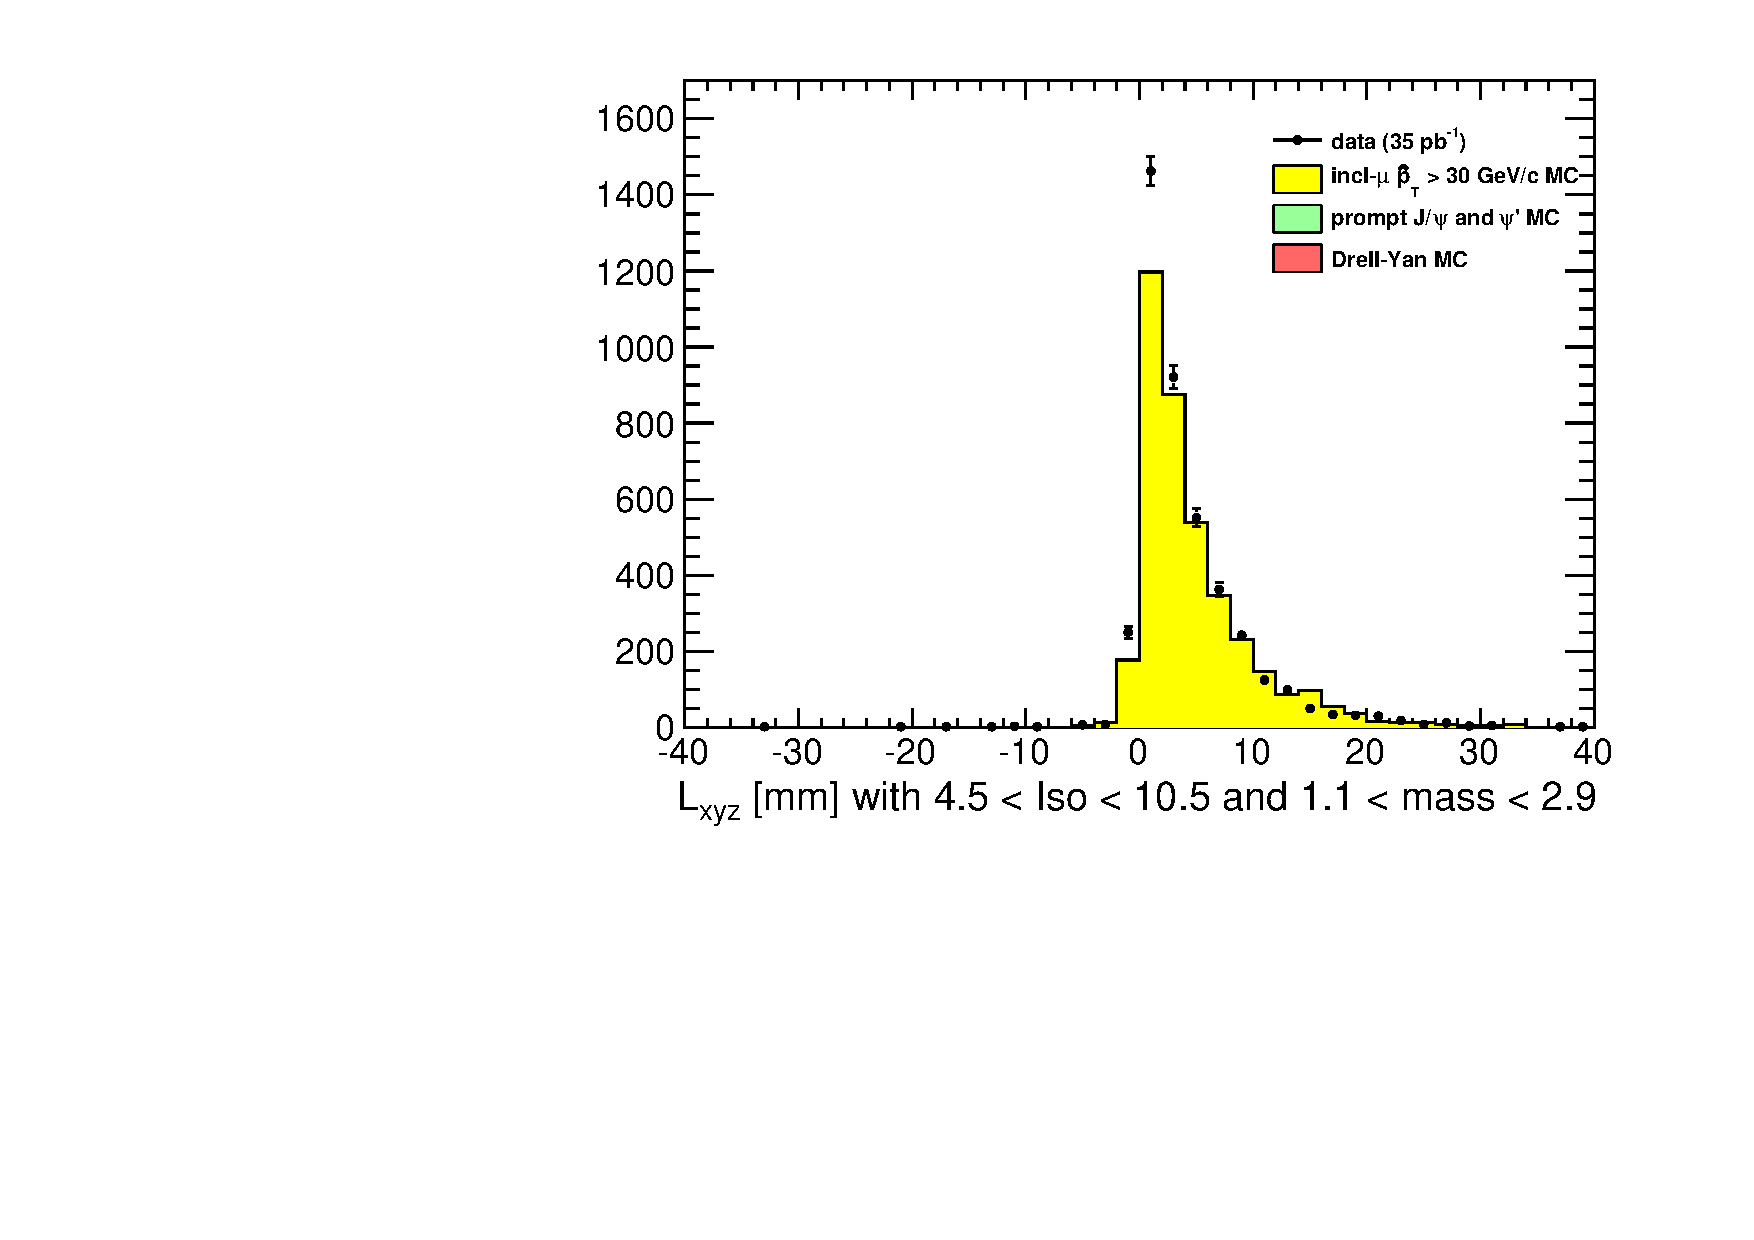
\includegraphics[width=\linewidth]{lowdimuon_lxyz_midmass_isosideband.pdf}

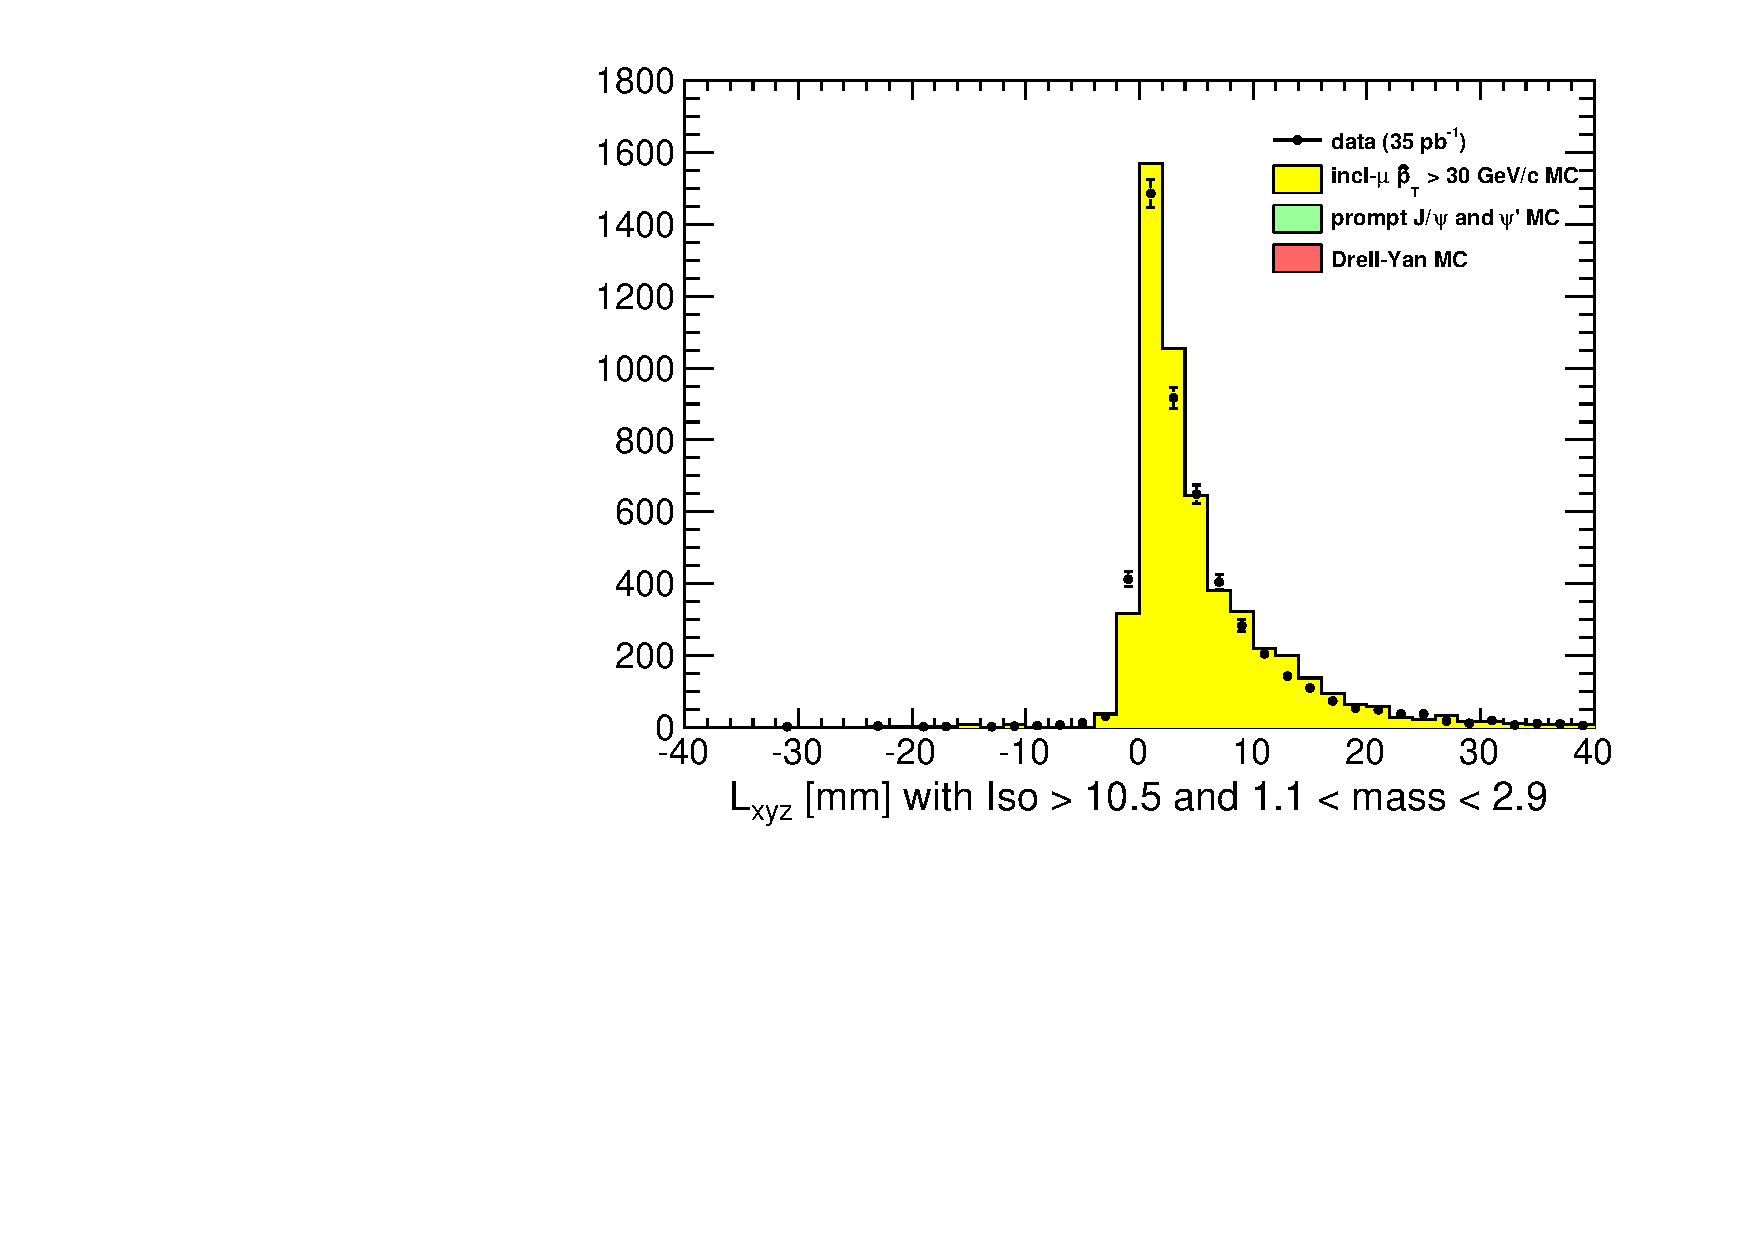
\includegraphics[width=\linewidth]{lowdimuon_lxyz_midmass_noniso.pdf}
\end{columns}
\end{frame}

\begin{frame}
\frametitle{Flight significance}

\begin{columns}
\column{0.6\linewidth}
\begin{itemize}
\item This is the mass $<$ 0.5~GeV/$c^2$ in $L_{xyz}$

\item Left edge (wrong-direction flights) is resolution; right tail is $\gamma c \tau$

\item Beampipe is at 30~mm ($\gamma \to \mu\mu$ conversions would
  happen primarily at the beampipe)
\end{itemize}

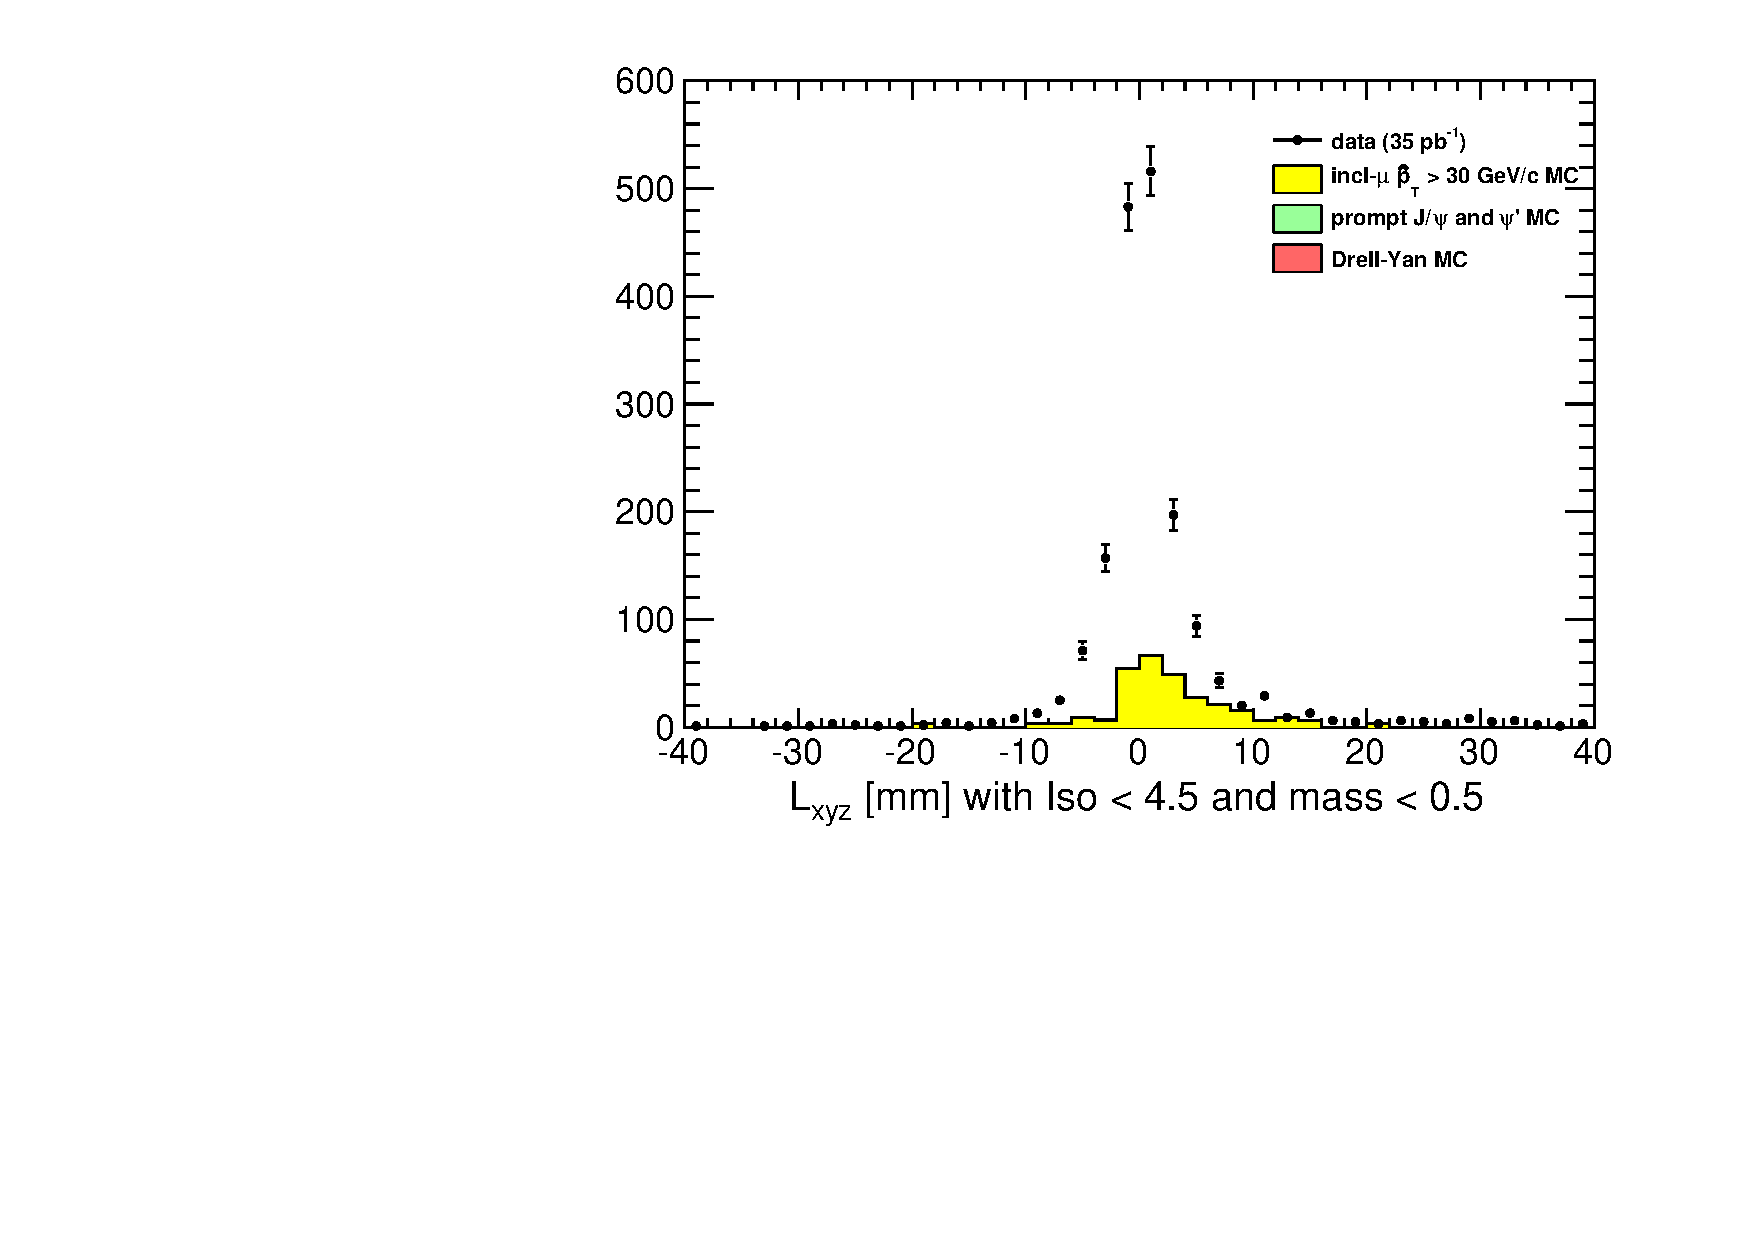
\includegraphics[width=\linewidth]{lowdimuon_lxyz_lowmass_isolated.pdf}

\column{0.4\linewidth}
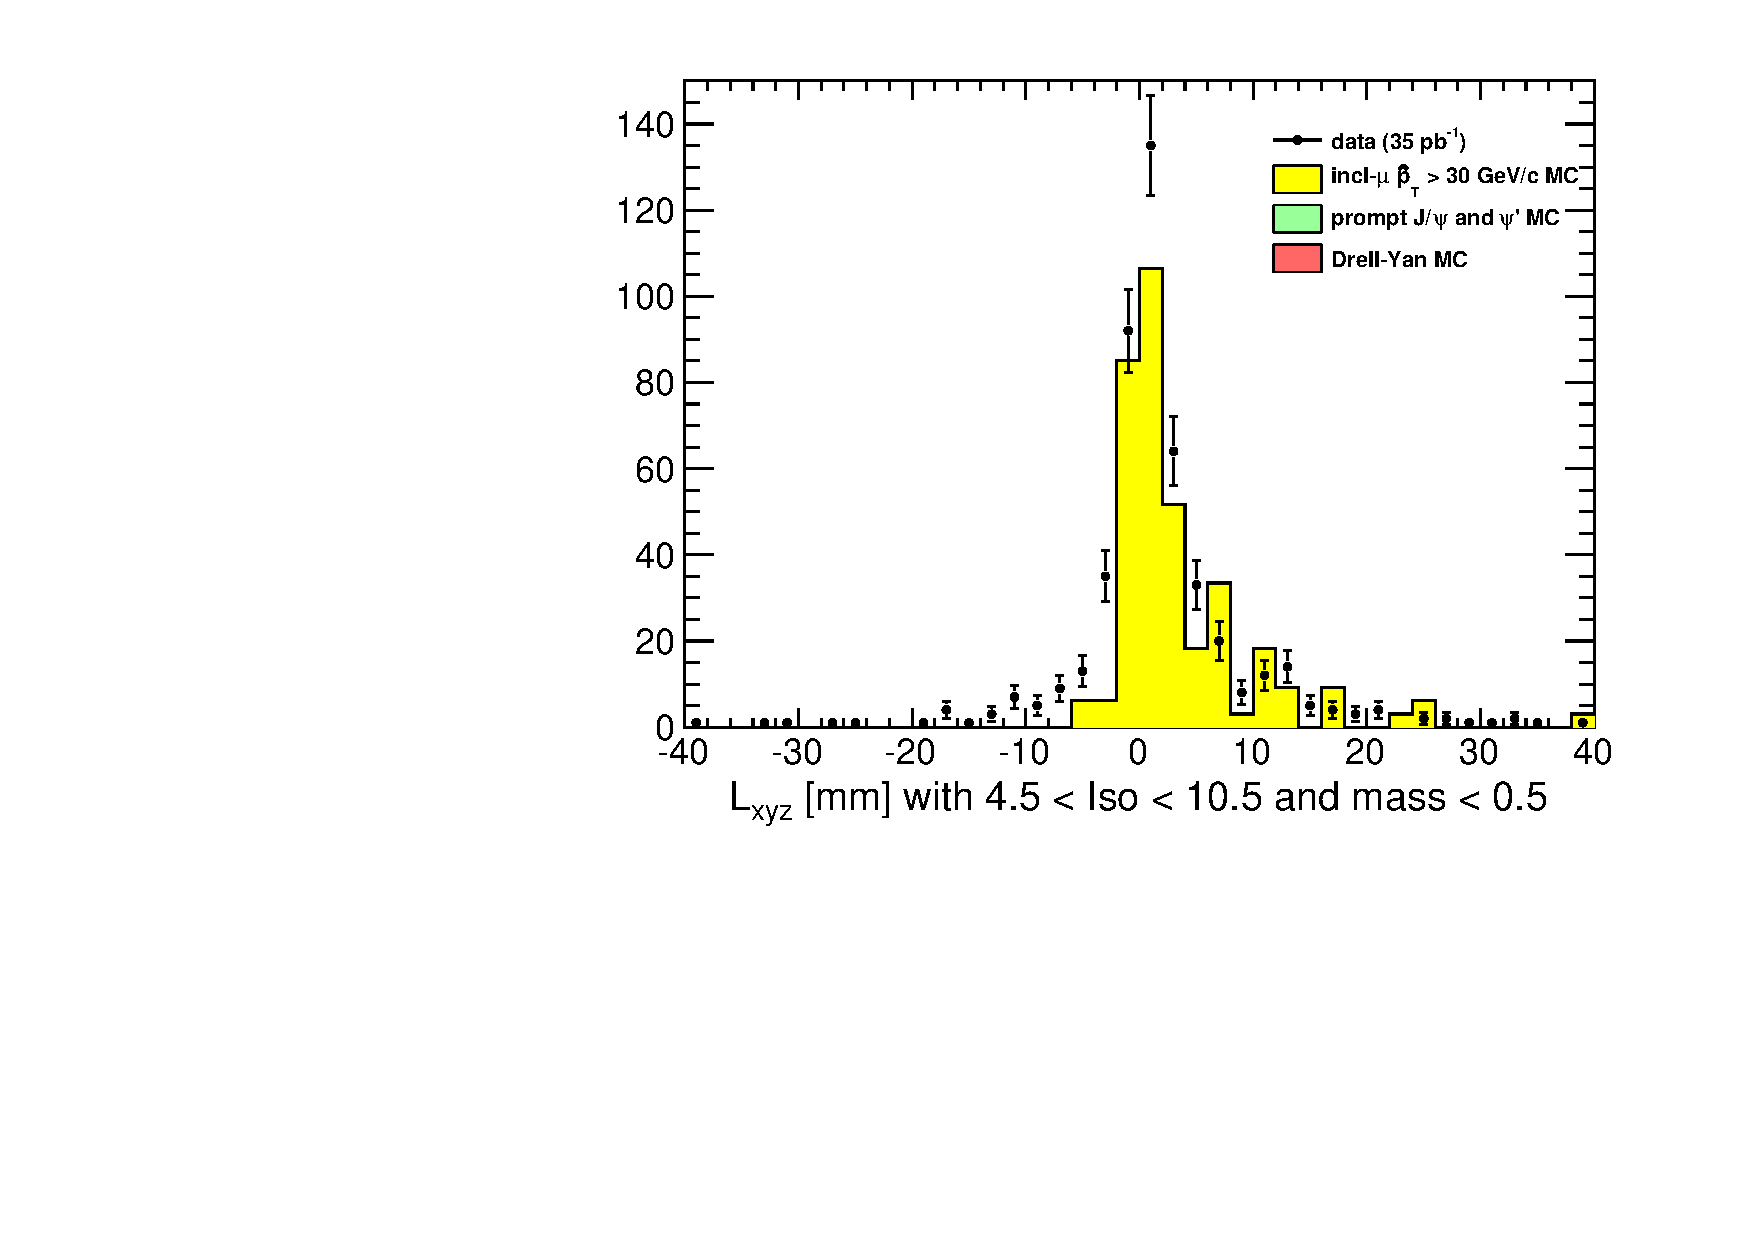
\includegraphics[width=\linewidth]{lowdimuon_lxyz_lowmass_isosideband.pdf}

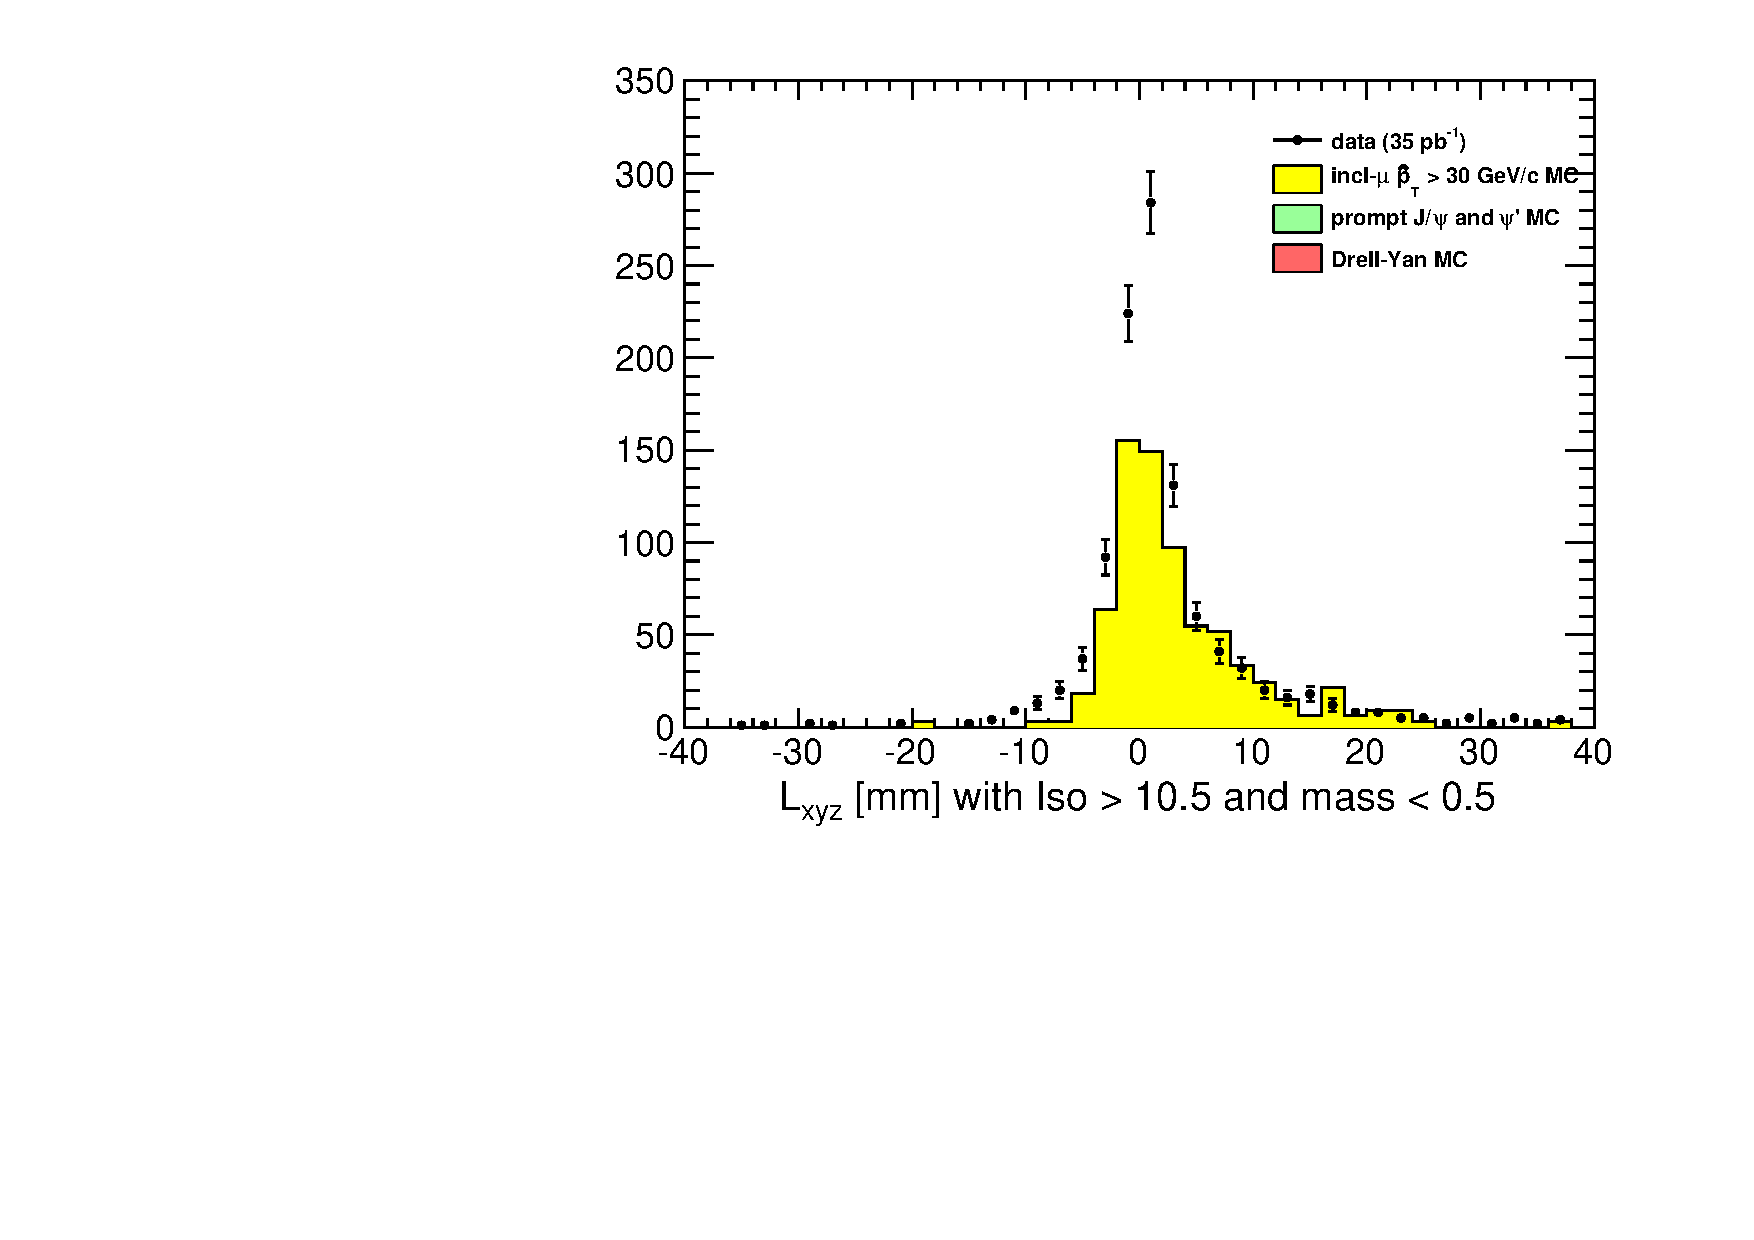
\includegraphics[width=\linewidth]{lowdimuon_lxyz_lowmass_noniso.pdf}
\end{columns}
\end{frame}

\begin{frame}
\frametitle{Flight significance}

\begin{columns}
\column{0.6\linewidth}
\begin{itemize}
\item Repeat for $L_{xy} = \vec{x}_\s{\tiny 2D} \cdot \vec{p}_\s{\tiny 2D} /
  |\vec{p}_\s{\tiny 2D}|$ in case you think there's a bias in using $z$
  because the closest primary vertex was identified using closeness in $z$

\item This is the 1.1 $<$ mass $<$ 2.9~GeV/$c^2$ continuum
\end{itemize}

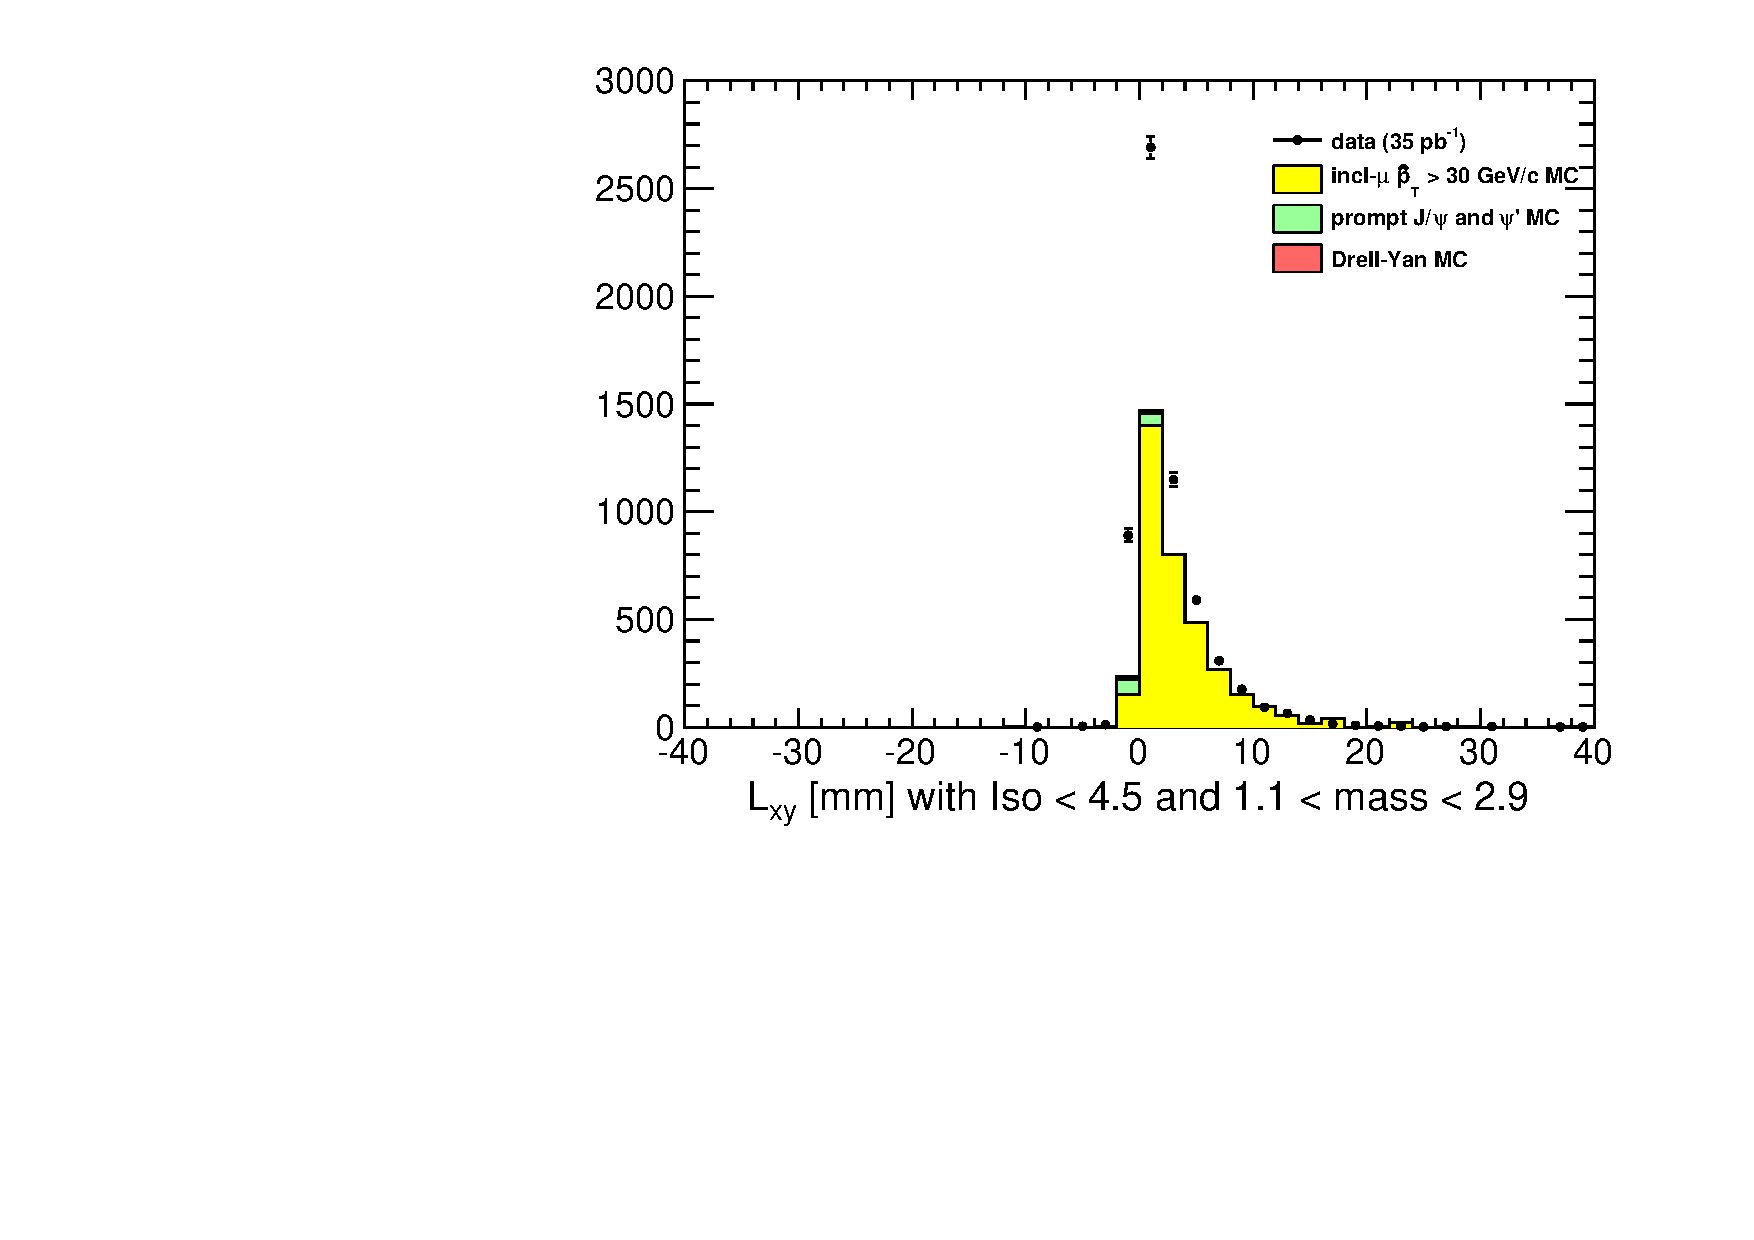
\includegraphics[width=\linewidth]{lowdimuon_lxy_midmass_isolated.pdf}

\column{0.4\linewidth}
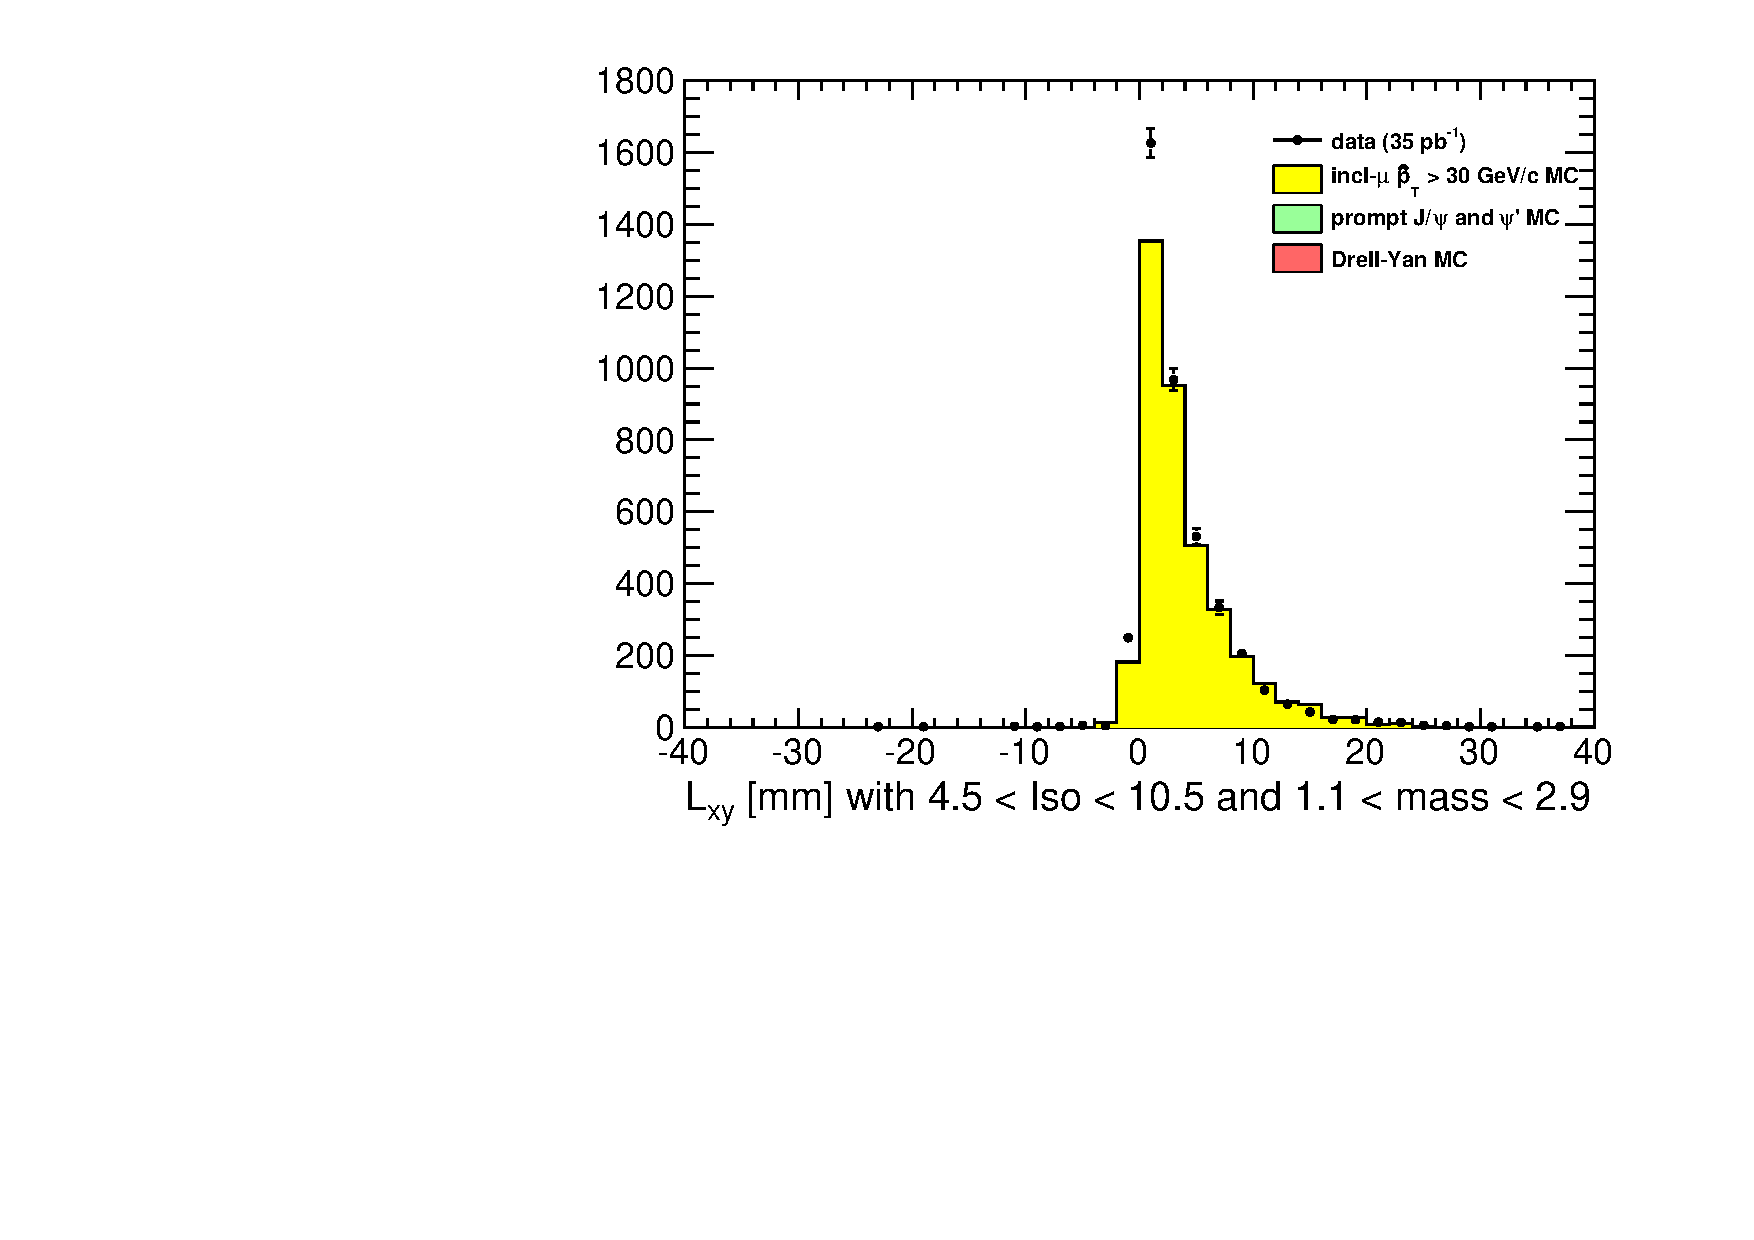
\includegraphics[width=\linewidth]{lowdimuon_lxy_midmass_isosideband.pdf}

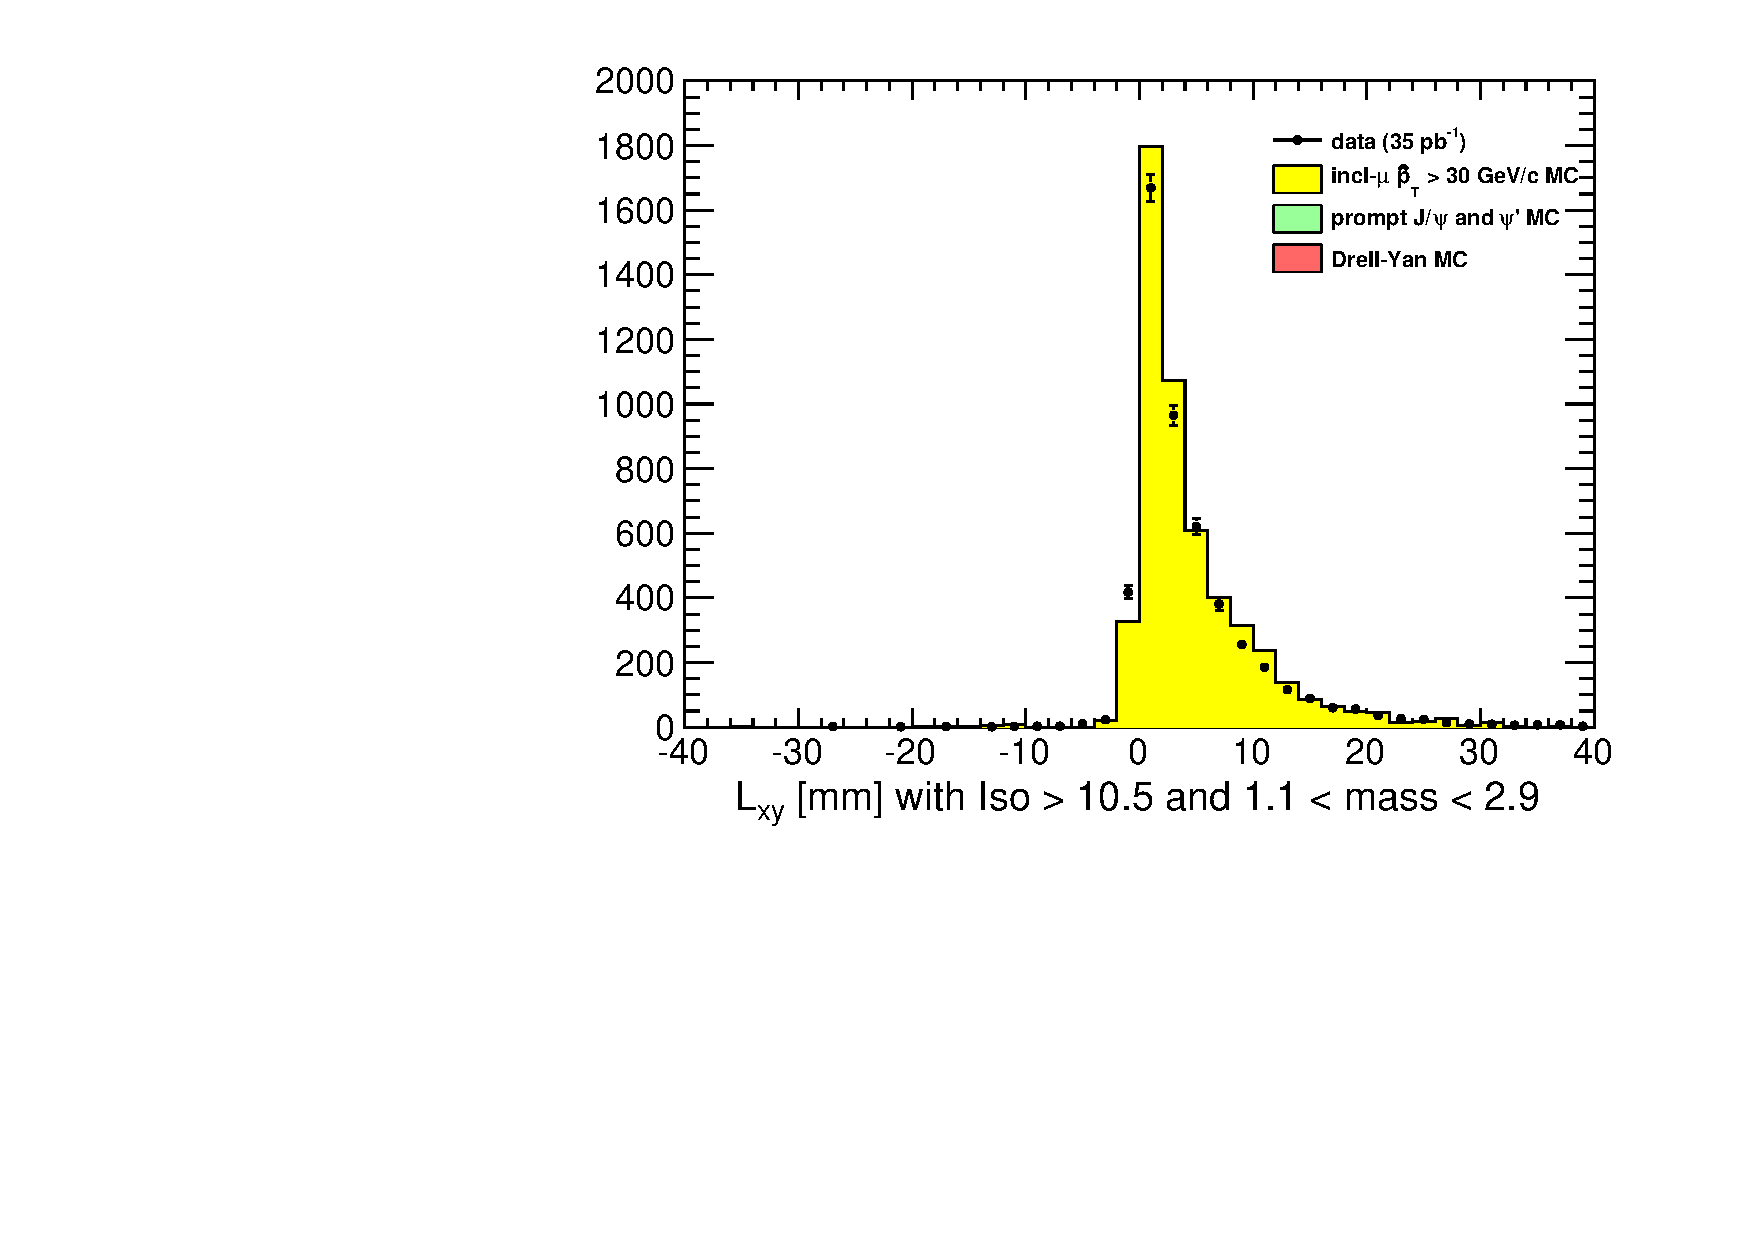
\includegraphics[width=\linewidth]{lowdimuon_lxy_midmass_noniso.pdf}
\end{columns}
\end{frame}

\begin{frame}
\frametitle{Flight significance}

\begin{columns}
\column{0.6\linewidth}
\begin{itemize}
\item Repeat for $L_{xy} = \vec{x}_\s{\tiny 2D} \cdot \vec{p}_\s{\tiny 2D} /
  |\vec{p}_\s{\tiny 2D}|$ in case you think there's a bias in using $z$
  because the closest primary vertex was identified using closeness in $z$

\item This is the mass $<$ 0.5~GeV/$c^2$ excess
\end{itemize}

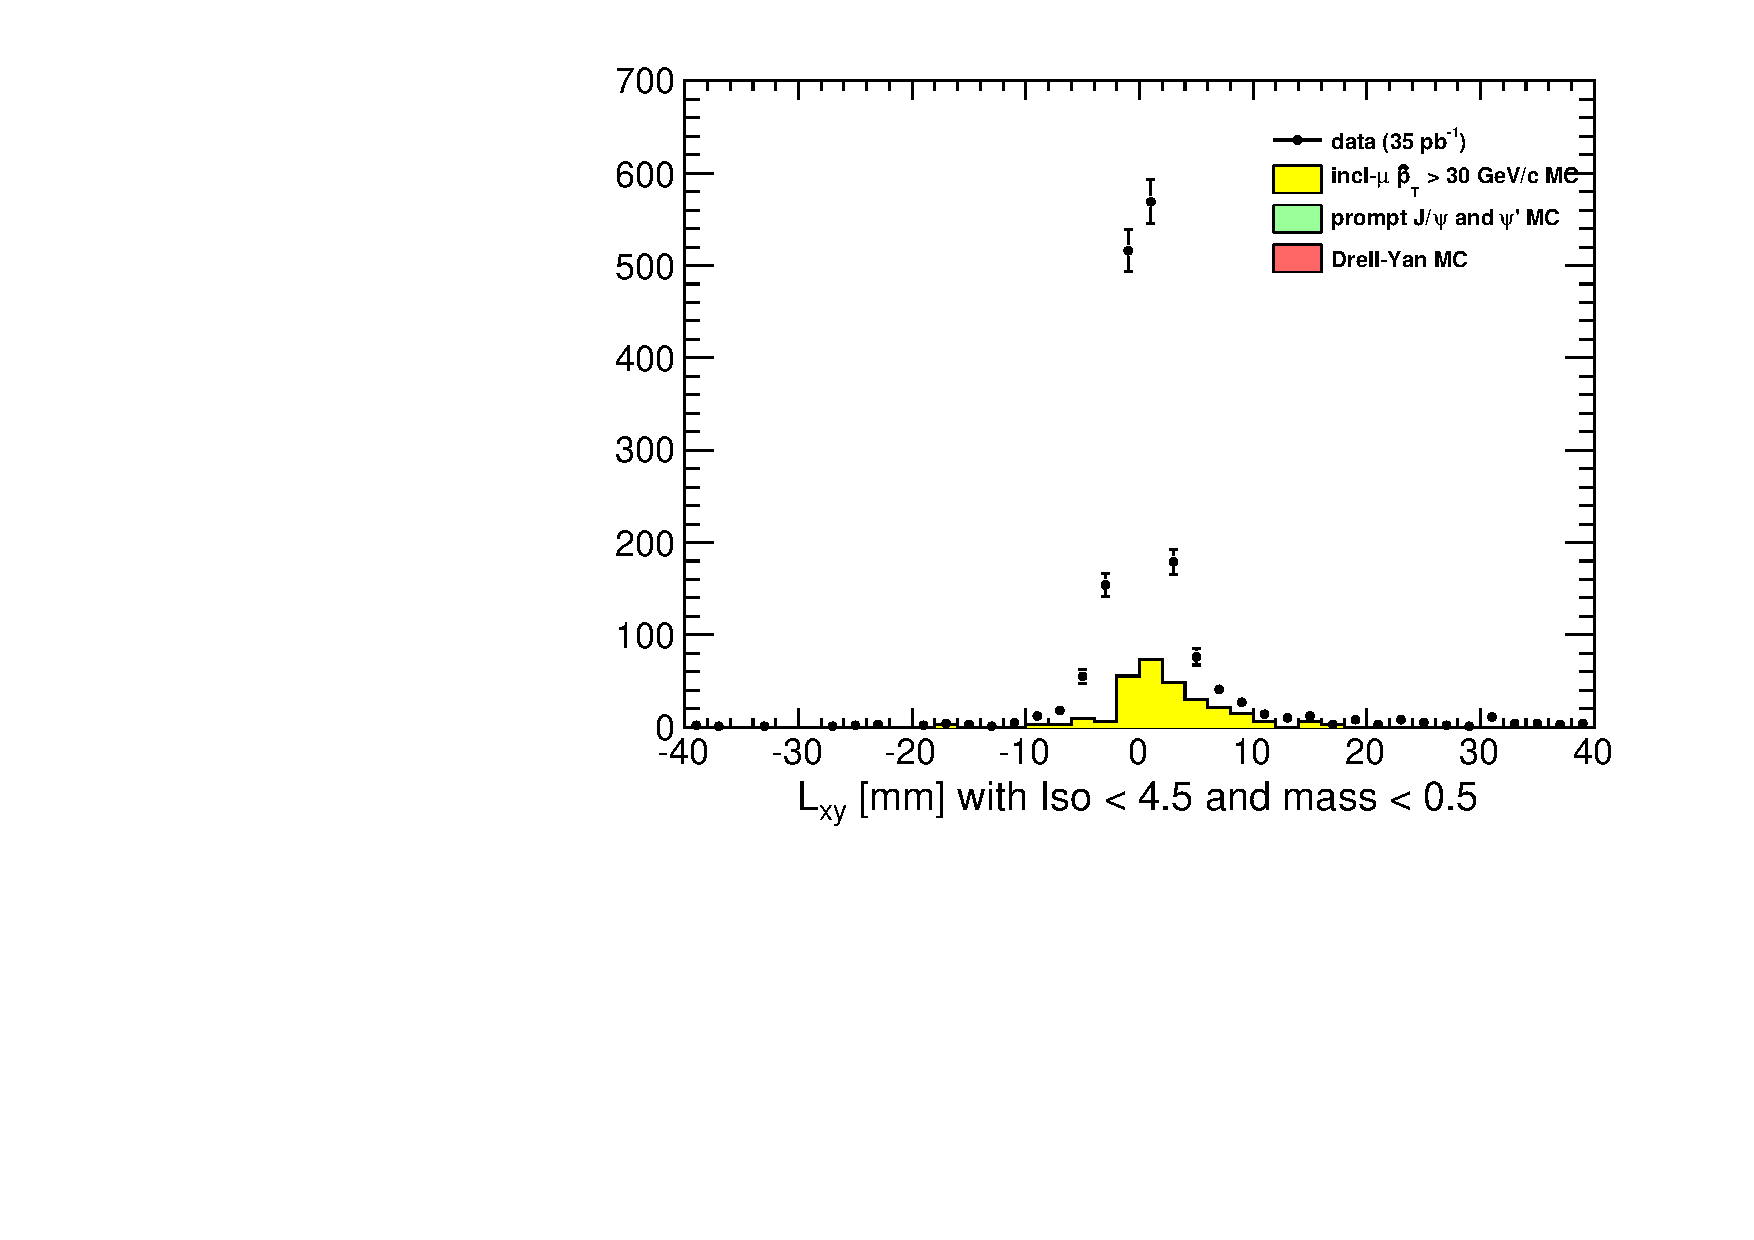
\includegraphics[width=\linewidth]{lowdimuon_lxy_lowmass_isolated.pdf}

\column{0.4\linewidth}
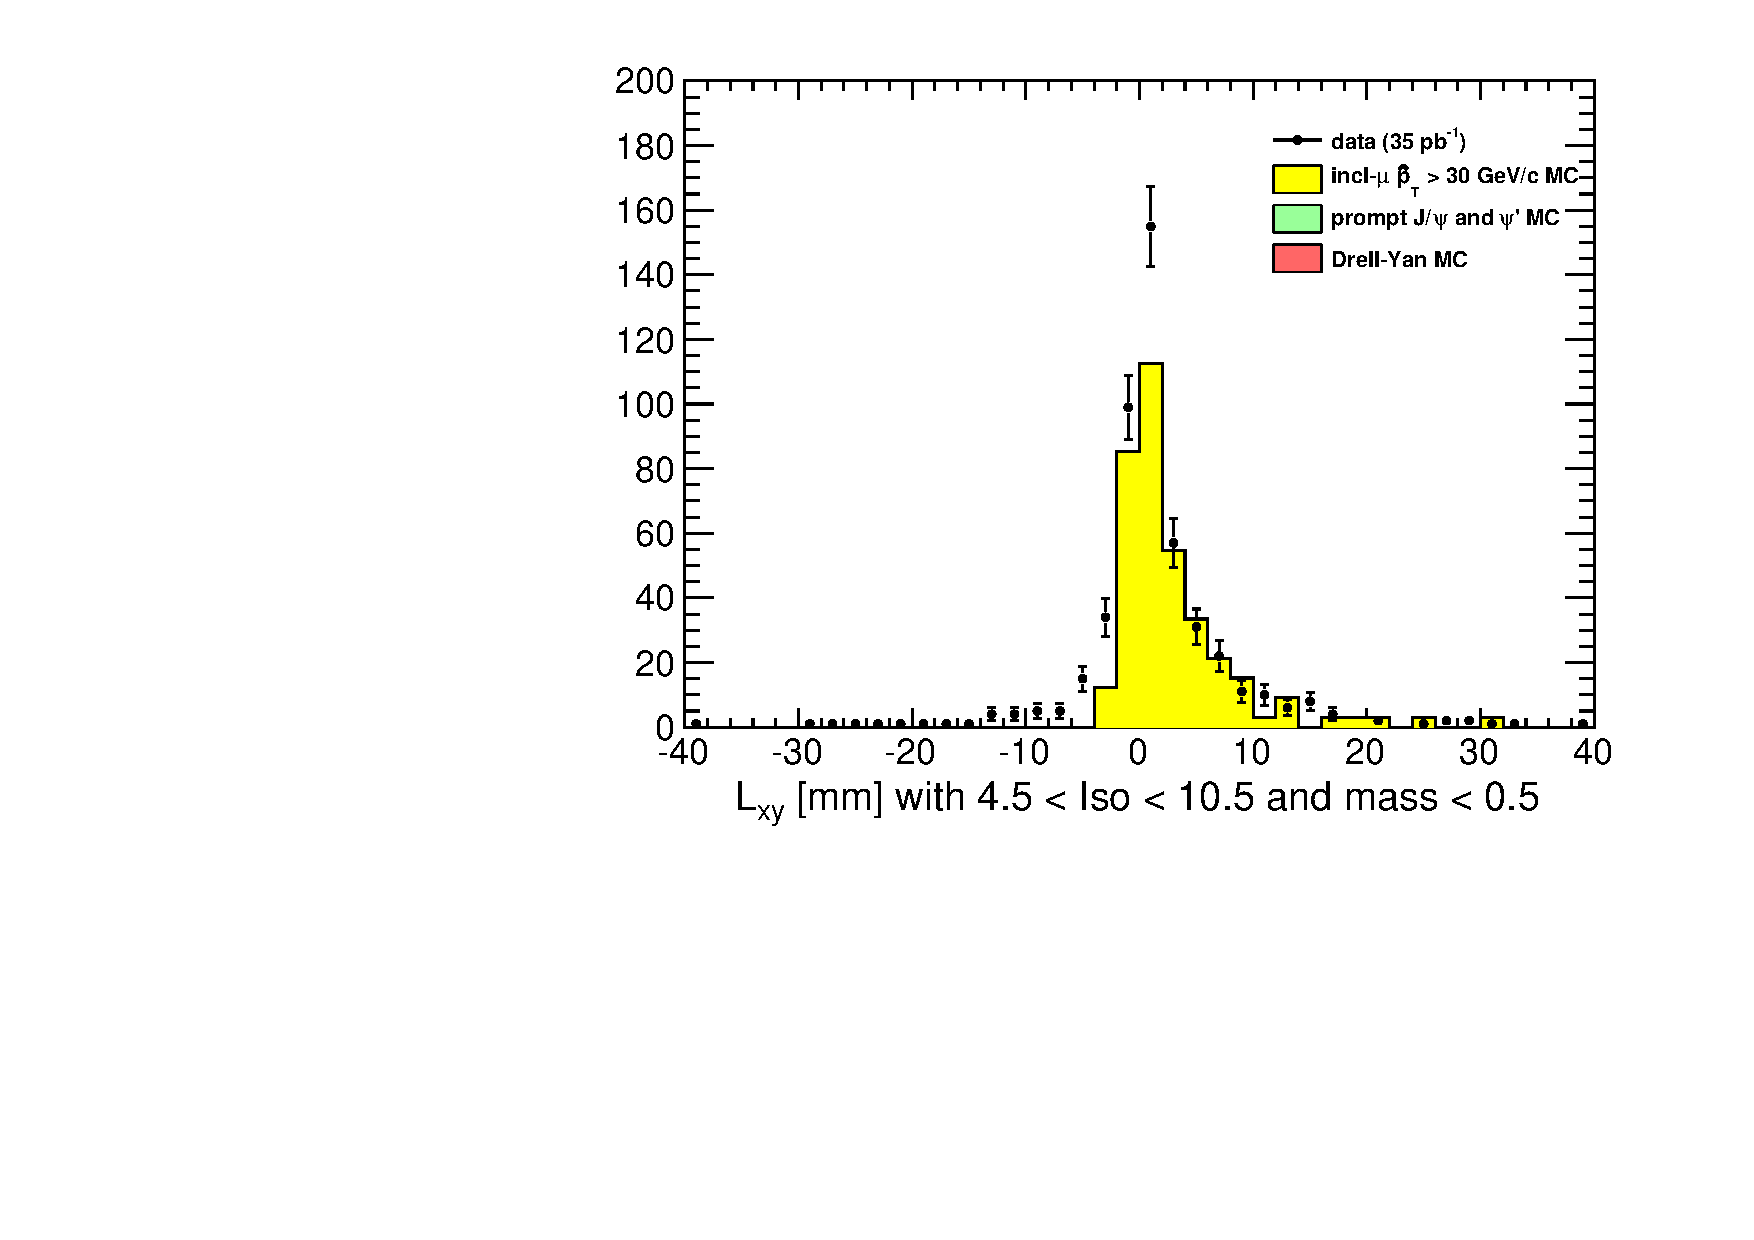
\includegraphics[width=\linewidth]{lowdimuon_lxy_lowmass_isosideband.pdf}

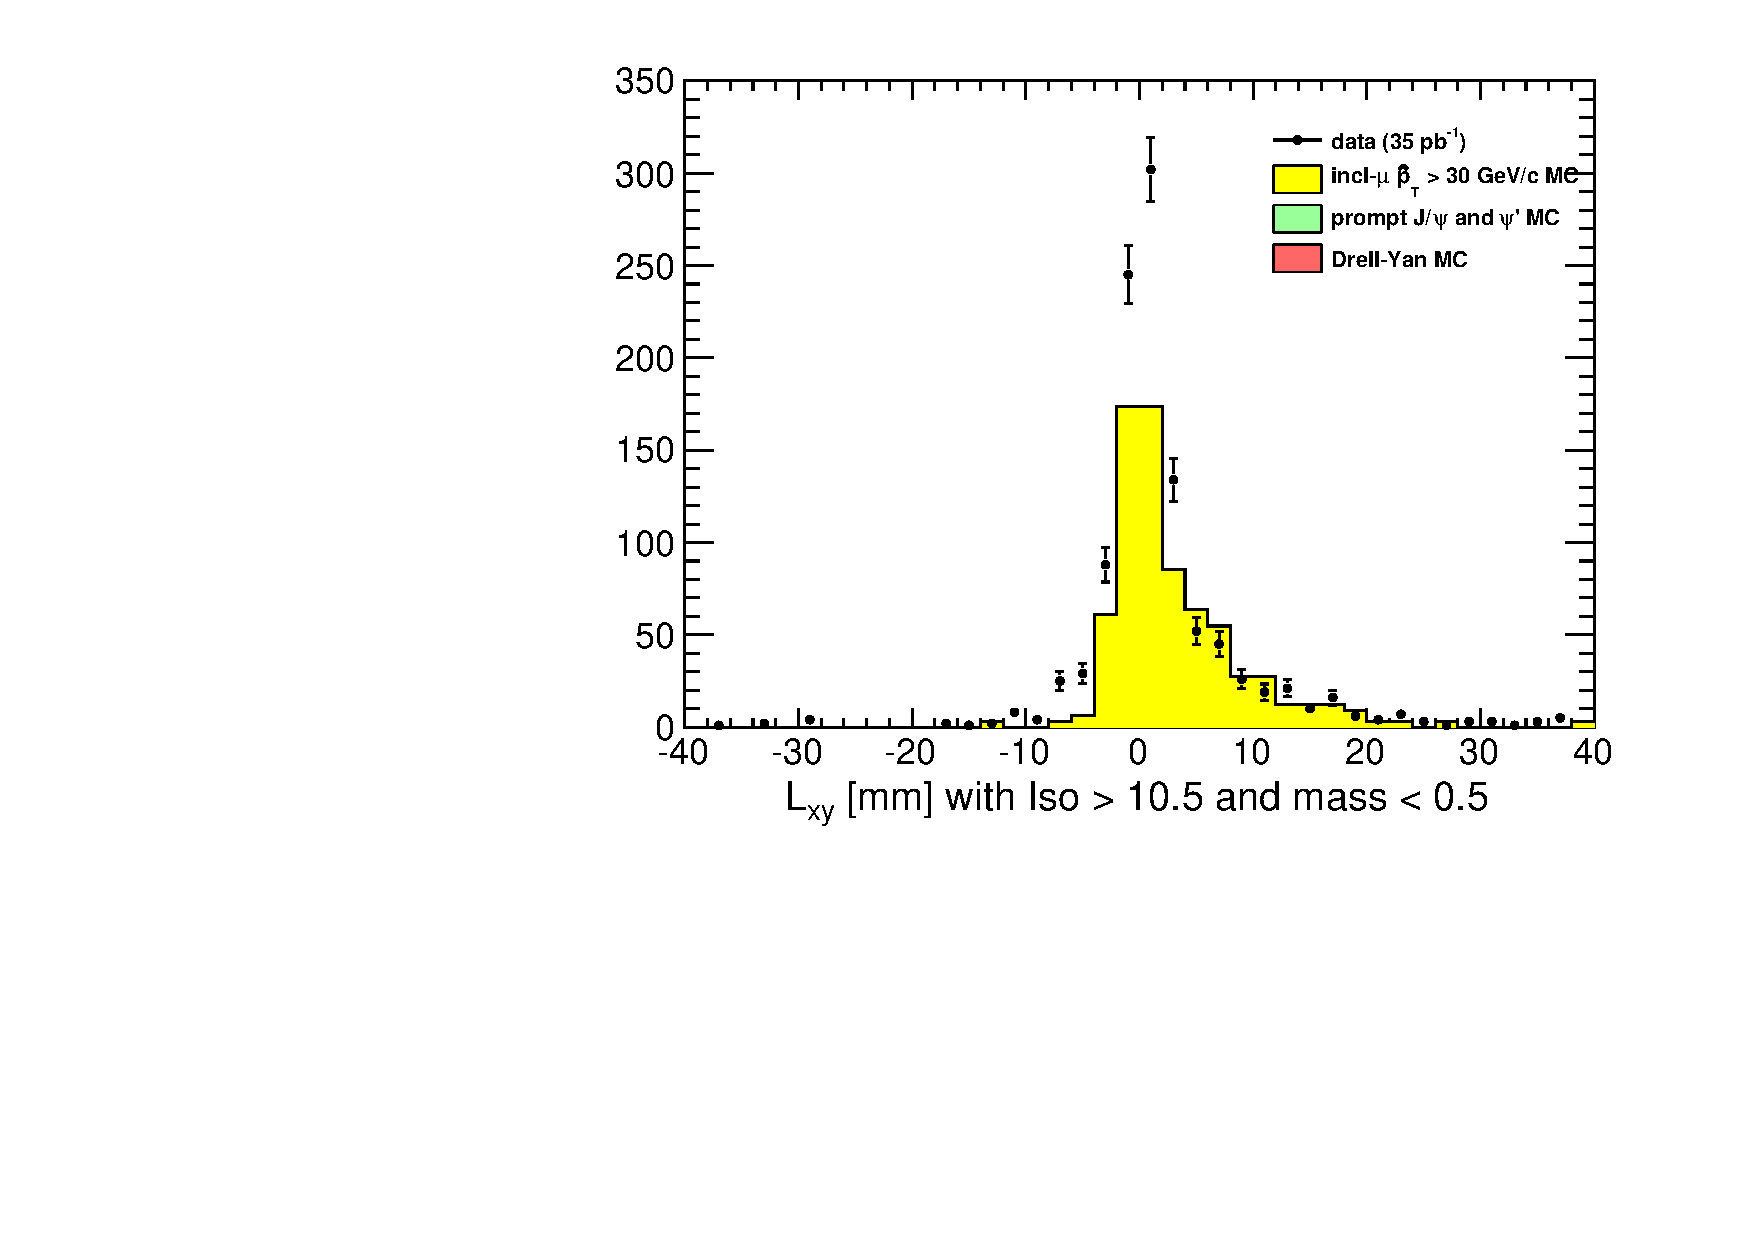
\includegraphics[width=\linewidth]{lowdimuon_lxy_lowmass_noniso.pdf}
\end{columns}
\end{frame}

\begin{frame}
\frametitle{What is certain}

\begin{itemize}
\item There's a significant class of events in data, not in this set
  of MC, with the following properties:
\begin{itemize}
\item isolated
\item real dimuons (not fake tracks or decays-in-flight or anything)
\item good vertex (not expected of all $b\bar{b}$)
\item appear at the origin (not expected of all $b\bar{b}$ or any $\gamma \to \mu\mu$ conversions)
\item a continuum and a sharp excess at low mass (too wide to be a resonance)
\end{itemize}

\item tried checking angular distribution of muons in the rest frame
  (check for vector versus uncorrelated), but this is highly sculpted
  by cuts
\end{itemize}

\vspace{0.3 cm}
\hspace{-0.83 cm} \textcolor{darkblue}{\Large What is likely}

\vspace{0.1 cm}
\begin{itemize}
\item The continuum, at least, is Drell-Yan--- there must be a problem
  with the Drell-Yan MC (privately generated, only change from
  official sample: 0 $<$ $\sqrt{s}$ $<$ 5~GeV/$c^2$ instead of 20 $<$
  $\sqrt{s}$ $<$ 40~GeV/$c^2$).
\end{itemize}
\end{frame}

\begin{frame}
\frametitle{Found a CDF paper on this}

\begin{itemize}
\item Use the same binning, same cuts:
\begin{itemize}
\item minimum $p_T$ by applying $\Delta R < 0.5$ (but still $p_T < 80$~GeV/$c$!)
\item ask for one $p_T > 20$~GeV/$c$ muon
\item for this plot, I {\it don't} rescale prompt $J/\psi$ by a factor of two
\end{itemize}
\end{itemize}

{\tt \scriptsize \url{http://www-cdf.fnal.gov/publications/cdf10013\_dimuon\_lowmasshighpt.pdf}}

\vspace{0.1 cm}
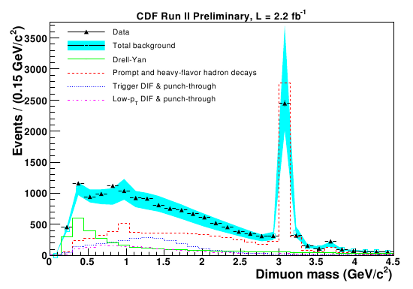
\includegraphics[width=0.5\linewidth]{cdf_highpt_dimuons.png}
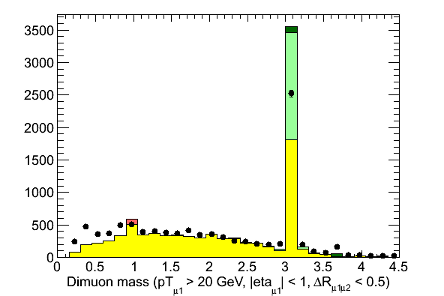
\includegraphics[width=0.5\linewidth]{our_highpt_dimuons.png}

\begin{itemize}
\item Their Drell-Yan Monte Carlo looks like our missing piece
\item Why is the yield similar???  (note difference in integrated luminosities: 2.2~fb$^{-1}$ vs.\ 0.035~fb$^{-1}$)
\end{itemize}

\label{numpages}
\end{frame}



%% \section*{First section}
%% \begin{frame}
%% \begin{center}
%% \Huge \textcolor{blue}{First section}
%% \end{center}
%% \end{frame}

\end{document}
